\section{Correction résiduelle absolue en \pT\ avec les événements \Gjets}\label{chapter-JERC-section-JES}
Durant ma thèse, j'étais responsable de la mesure de cette correction avec les événements \Gjets\ pour les années 2018 et 2017-UL pour la collaboration CMS.
Cette section présente la sélection des événements \Gjets, leur analyse et les derniers résultats obtenus pour l'année 2018.
\subsection{Événements utilisés}\label{chapter-JERC-section-JES-subsec-evt_select}
\subsubsection{Ensembles d'événements analysés}
%18 data
%     Run2018A-17Sep2018-v2
%     /EGamma/Run2018A-17Sep2018-v2/MINIAOD
%     13654.355526985
%     
%     Run2018B-17Sep2018-v1
%     /EGamma/Run2018B-17Sep2018-v1/MINIAOD
%     7057.825158567
%     
%     Run2018C-17Sep2018-v1
%     /EGamma/Run2018C-17Sep2018-v1/MINIAOD
%     6894.770971269
%     
%     Run2018D-PromptReco-v2
%     /EGamma/Run2018D-PromptReco-v2/MINIAOD
%     31066.589629726
%
%18 MC
%     GJet_Pt-15To6000_RunIIAutumn18MiniAOD-102X
%     /GJet_Pt-15To6000_TuneCP5-Flat_13TeV_pythia8/RunIIAutumn18MiniAOD-102X_upgrade2018_realistic_v15-v1/MINIAODSIM
%     283000.0
%
%17UL data
%     Run2017B-09Aug2019_UL2017-v1
%     /SinglePhoton/Run2017B-09Aug2019_UL2017-v1/MINIAOD
%     4793.961426839
%     
%     Run2017C-09Aug2019_UL2017-v1
%     /SinglePhoton/Run2017C-09Aug2019_UL2017-v1/MINIAOD
%     9631.214820913
%     
%     Run2017D-09Aug2019_UL2017-v1
%     /SinglePhoton/Run2017D-09Aug2019_UL2017-v1/MINIAOD
%     4247.682053046
%     
%     Run2017E-09Aug2019_UL2017-v1
%     /SinglePhoton/Run2017E-09Aug2019_UL2017-v1/MINIAOD
%     9313.642401775
%     
%     Run2017F-09Aug2019_UL2017-v1
%     /SinglePhoton/Run2017F-09Aug2019_UL2017-v1/MINIAOD
%     13539.378417564
%
%
%17UL MC
%     GJets_HT-40To100_RunIISummer19MiniAOD-106X
%     /GJets_HT-40To100_TuneCP5_13TeV-madgraphMLM-pythia8/RunIISummer19UL17MiniAOD-106X_mc2017_realistic_v6-v1/MINIAODSIM
%     18700.0
%     
%     GJets_HT-100To200_RunIISummer19MiniAOD-106X
%     /GJets_HT-100To200_TuneCP5_13TeV-madgraphMLM-pythia8/RunIISummer19UL17MiniAOD-4cores5k_106X_mc2017_realistic_v6-v1/MINIAODSIM
%     8640.0
%     
%     GJets_HT-200To400_RunIISummer19MiniAOD-106X
%     /GJets_HT-200To400_TuneCP5_13TeV-madgraphMLM-pythia8/RunIISummer19UL17MiniAOD-106X_mc2017_realistic_v6-v1/MINIAODSIM
%     2185.0
%     
%     GJets_HT-400To600_RunIISummer19MiniAOD-106X
%     /GJets_HT-400To600_TuneCP5_13TeV-madgraphMLM-pythia8/RunIISummer19UL17MiniAOD-106X_mc2017_realistic_v6-v1/MINIAODSIM
%     259.9
%     
%     GJets_HT-600ToInf_RunIISummer19MiniAOD-106X
%     /GJets_HT-600ToInf_TuneCP5_13TeV-madgraphMLM-pythia8/RunIISummer19UL17MiniAOD-106X_mc2017_realistic_v6-v1/MINIAODSIM
%     85.31 \pm 0.2564
\paragraph{Données}
Les jeux de données utilisés pour 2018 et 2017-UL sont basés sur la présence d'un photon dans l'état final.
Pour chacune de ces années, plusieurs périodes (\emph{runs}) sont considérées, celles des collisions \proton\proton, dont la liste et les luminosités correspondantes sont présentées dans le tableau~\ref{tab-Runs_and_lumis_2018_and_2017UL_GJet}.
La liste détaillée de ces jeux de données se trouve dans l'annexe~\refApJERCdatasets.
\begin{table}[h]
\centering
\begin{tabular}{ccc}
\toprule
\multirow{2}{*}{Run} & \multicolumn{2}{c}{Luminosité (\SI{}{\femto\barn^{-1}})} \\
\cmidrule(lr){2-3}
 & 2018 & 2017-UL \\
\midrule
A & \num{13.98} & - \\
B & \num{7.06} & \num{4.823} \\
C & \num{6.90} & \num{9.664} \\
D & \num{31.75} & \num{4.252} \\
E & - & \num{9.278} \\
F & - & \num{13.54} \\
\midrule
Total & \num{59.69} & \num{41.56} \\
\bottomrule
\end{tabular}
\caption{Liste des périodes de prise de données considérées et luminosités correspondantes.}
\label{tab-Runs_and_lumis_2018_and_2017UL_GJet}
\end{table}
\paragraph{Simulations}
Les simulations utilisées contiennent des événements \Gjets\ de type $\quark\gluon\to\quark\photon$, comme ceux des figures~\ref{subfig-fgraph-gq_qGamma_S} et~\ref{subfig-fgraph-gq_qGamma_T}, et $\quark\quark\to\gluon\photon$, comme celui de la figure~\ref{subfig-fgraph-qq_gGamma}.
Pour l'année 2018, les événements sont générés en un seul jeu de données
à l'aide de \PYTHIA~8~\cite{pythia8.2}
avec les réglages CP5-Flat~\cite{tunes_2019}
et une énergie dans le centre de masse de \SI{13}{\TeV}.
Dans l'état final, un photon d'impulsion transverse comprise entre \num{15} et \SI{6000}{\GeV} est généré.
Pour l'année 2017-UL, les événements sont générés conjointement
à l'aide de \PYTHIA~8~\cite{pythia8.2}
avec les réglages CP5~\cite{tunes_2019}
et
\MADGRAPHc~\cite{madgraph5}
et une énergie dans le centre de masse de \SI{13}{\TeV}.
Dans l'état final, la somme scalaire des impulsions transverses des jets, notée HT, appartient à un intervalle, définissant ainsi cinq jeux de données.
Les sections efficaces des événements simulés ainsi obtenus sont présentées dans le tableau~\ref{tab-MC_xsec_2018_and_2017UL_GJet}.
La liste détaillée de ces jeux de données simulées se trouve dans l'annexe~\refApJERCdatasets.
\begin{table}[h]
\centering
\begin{tabular}{clc}
\toprule
Année & Caractéristique & Section efficace (\SI{}{\pico\barn})\\
\midrule
2018 & $\pT^{\photon}\in [\num{15}, \num{6000}]\usp\SI{}{\GeV}$ & \num{283000.0}\\
2017-UL & $\text{HT} \in [\num{40}, \num{100}]\usp\SI{}{\GeV}$ & \num{18700.0} \\
2017-UL & $\text{HT} \in [\num{100}, \num{200}]\usp\SI{}{\GeV}$ & \num{8640.0} \\
2017-UL & $\text{HT} \in [\num{200}, \num{400}]\usp\SI{}{\GeV}$ & \num{2185.0} \\
2017-UL & $\text{HT} \in [\num{400}, \num{600}]\usp\SI{}{\GeV}$ & \num{259.9} \\
2017-UL & $\text{HT} > \SI{600}{\GeV}$ & \num{85.31} \\
\bottomrule
\end{tabular}
\caption{Sections efficaces des différents événements \Gjets\ simulés.}
\label{tab-MC_xsec_2018_and_2017UL_GJet}
\end{table}
\subsubsection{Sélection des événements}
Une sélection des événements à considérer est réalisée lors de l'analyse.
En effet, les événements souhaités sont ceux contenant un photon avec un ou plusieurs jets;
un des bruits de fond principal provient d'événements multijet où un des jets est identifié à tort comme un photon.
Cette situation peut arriver lorsqu'une fraction importante de l'énergie de ce jet est portée par un ou plusieurs pions neutres, les \pionnull.
Les \pionnull\ se propagent sur des distances moyennes de \SI{26}{\nano\meter} puis se désintègrent dans \SI{99}{\%} des cas en deux photons~\cite{PDG_booklet_2020}.
Ces particules ne laissent donc aucune trace dans le trajectographe et un dépôt d'énergie dans le ECAL, tout comme les photons issus de l'interaction initiale.
Un tel jet comporte ainsi une signature similaire à un photon d'un événement \Gjet\ autour duquel une activité hadronique existe.
%Les topologies de ces deux types d'événements, semblables, sont représentées sur la figure~\ref{fig-Gamma_plus_jet_events_real_faked}.
%\begin{figure}[h]
%\centering
%\subcaptionbox{Topologie d'un événement dijet, dont un jet contient de nombreux \pionnull.\label{subfig-Gamma_plus_jet_basic_event_dijet_faked}}[.45\textwidth]
%{\includegraphics[width=.45\textwidth,height=.25\textheight,keepaspectratio]{\PhDthesisdir/plots_and_images/Event_displays/JERC/Dijets_pi0s.tex}}
%\hfill
%\subcaptionbox{Topologie d'un vrai événement \Gjet\ avec un peu d'activité hadronique autour du photon.\label{subfig-Gamma_plus_jet_basic_event_real}}[.45\textwidth]{\includegraphics[width=.45\textwidth,height=.25\textheight,keepaspectratio]{\PhDthesisdir/plots_and_images/Event_displays/JERC/Gamma_plus_jet_hadronic_noise.tex}}
%\caption{Topologies d'événements \Gjet\ et dijet.}
%\label{fig-Gamma_plus_jet_events_real_faked}
%\end{figure}
\paragraph{Sélection sur les photons}
Une sélection des photons est appliquée afin de réduire le bruit de fond.
La collaboration CMS propose des critères d'identification des photons (lâche, moyen et strict) s'appuyant sur diverses propriétés du \og candidat \fg{} photon:
\begin{itemize}
\item $H/E_{SC}$ est le rapport de l'énergie hadronique dans un cône de $\Delta R < \num{0.15}$ autour du photon sur l'énergie du \emph{supercluster}, défini dans le chapitre~\refChLHCCMS.
Un photon est sensé déposer son énergie dans le ECAL et ne laisser aucun signal dans le HCAL.
Une faible valeur de $H/E_{SC}$ est donc compatible avec un photon.
\item $\sigma_{i\eta i\eta}$ est l'étalement en $\eta$ du dépôt d'énergie dans le ECAL.
Cette observable est reliée à la forme de la gerbe électromagnétique.
Un seuil maximal sur $\sigma_{i\eta i\eta}$ est imposé pour l'identification des photons.
\item $I_{CH}$ est l'isolation vis-à-vis des hadrons chargés.
Elle se définit comme le ratio entre la somme des impulsions transverses de tous les hadrons chargés situés à une distance $\Delta R$ du candidat photon dans le plan $(\eta,\phi)$ inférieure à \num{0.3} et l'impulsion transverse du candidat photon lui-même.
\item $I_{NH}$ est l'isolation vis-à-vis des hadrons neutres, analogue à $I_{CH}$.
\item $I_{\photon}$ est l'isolation vis-à-vis des photons autres que le candidat lui-même, analogue à $I_{CH}$.
\end{itemize}
À cet ensemble de variables dont une valeur maximale est admise pour l'identification des photons s'ajoute $R_9$, définie comme
\begin{equation}
R_9 = \frac{E_{3\times3}}{E_{SC}}
\label{eq-R9_definition}
\end{equation}
avec
$E_{3\times3}$ la somme des énergies dans les cristaux du ECAL formant un carré de trois cristaux de côté centré sur le cristal contenant le plus d'énergie dans le \emph{supercluster}.
et
$E_{SC}$
l'énergie du \emph{supercluster}~\cite{photon_ID_2015}.
Dans l'analyse des événements \Gjets, il est demandé que $R_9 > \num{0.90}$.
\par Les variables d'isolation sont corrigées afin de prendre en compte l'empilement.
L'isolation corrigée $I^\text{corr}$ s'exprime ainsi en fonction de l'isolation $I$ comme
\begin{equation}
I^\text{corr} = \max\left( I - \rho \times \mathcal{E_A} , 0\right)
\end{equation}
où $\mathcal{E_A}$ est l'aire effective, \ie\ la fraction de l'espace $(\eta,\phi)$ correspondant à la zone d'isolation à corriger pour l'empilement. Les valeurs des aires effectives utilisées sont présentées dans le tableau~\ref{tab-CutBasedPhotonIdentificationRun2-effective_areas}.
\begin{table}[h]
\centering
\begin{tabular}{cccc}
\toprule
Région & Hadrons chargés & Hadrons neutres & Photons \\
\midrule
$\abs{\eta} \leq \num{1.0}$ & \num{0.0112} & \num{0.0668} & \num{0.1113} \\
$\num{1.0} < \abs{\eta} \leq \num{1.479}$ & \num{0.0108} & \num{0.1054} & \num{0.0953} \\
$\num{1.479} < \abs{\eta} \leq \num{2.0}$ & \num{0.0106} & \num{0.0786} & \num{0.0619} \\
$\num{2.0} < \abs{\eta} \leq \num{2.2}$ & \num{0.01002} & \num{0.0233} & \num{0.0837} \\
$\num{2.2} < \abs{\eta} \leq \num{2.3}$ & \num{0.0098} & \num{0.0078} & \num{0.1070} \\
$\num{2.3} < \abs{\eta} \leq \num{2.4}$ & \num{0.0089} & \num{0.0028} & \num{0.1212} \\
$\abs{\eta} > \num{2.4}$ & \num{0.0087} & \num{0.0137} & \num{0.1466} \\
\bottomrule
\end{tabular}
\caption[Aires effectives de correction de l'isolation du photon.]{Valeurs de l'aire effective $\mathcal{E_A}$ utilisée pour corriger la contribution de l'empilement aux isolations des photons vis-à-vis des autres particules.}
\label{tab-CutBasedPhotonIdentificationRun2-effective_areas}
\end{table}
\par De plus, un veto est appliqué aux photons pouvant être reliés à une trace dans le trajectographe.
Ce veto permet de limiter la contamination des photons considérés dans l'analyse par des électrons reconstruits à tort comme des photons.
Les coupures correspondant aux différents critères d'identification des photons ainsi que leurs efficacités d'identification et de réjection sont résumées dans le tableau~\ref{tab-CutBasedPhotonIdentificationRun2}.
\begin{table}[h]
\centering\small
\begin{tabularx}{\textwidth}{Xcccccc}
\toprule
Critère & \multicolumn{2}{c}{Lâche} & \multicolumn{2}{c}{Moyen} & \multicolumn{2}{c}{Strict} \\
\cmidrule(lr){2-3}\cmidrule(lr){4-5}\cmidrule(lr){6-7}
Région & Barillet & Bouchon & Barillet & Bouchon & Barillet & Bouchon\\
\midrule
Efficacité & \SI{90.08}{\%} & \SI{90.65}{\%} & \SI{80.29}{\%} & \SI{80.08}{\%} & \SI{70.24}{\%} & \SI{70.13}{\%} \\
Réjection & \SI{86.25}{\%} & \SI{76.72}{\%} & \SI{89.36}{\%} & \SI{81.85}{\%} & \SI{90.97}{\%} & \SI{84.55}{\%} \\
\midrule
$H/E_{SC}$ & \num{0.04596} & \num{0.0590} & \num{0.02197} & \num{0.0326} & \num{0.02148} & \num{0.0321} \\
$\sigma_{i\eta i\eta}$ & \num{0.0106} & \num{0.0272} & \num{0.01015} & \num{0.0272} & \num{0.00996} & \num{0.0271} \\
$I_{CH}^\text{corr}$ & \num{1.694} & \num{2.089} & \num{1.141} & \num{1.051} & \num{0.65} & \num{0.517} \\
\multirow{3}{*}{$I_{NH}^\text{corr} \!\!\!\hphantom{I_{\photon}^\text{corr}} \left\lbrace \begin{matrix} \vphantom{0} \\ \vphantom{0} \\ \vphantom{0} \end{matrix} \right. $} & $\num{24.032}$& $\num{19.722}$& $\num{1.189}$& $\num{2.718}$& $\num{0.317}$& $\num{2.716}$\\
& $+ \num{0.01512} \, \pT$& $+ \num{0.011} \, \pT$& $+ \num{0.01512} \, \pT$& $+ \num{0.0117} \, \pT$& $+ \num{0.01512} \, \pT$& $+ \num{0.0117} \, \pT$ \\
& $+ \num{2.259} \pT^{\!2} \! / 10^5$ & $+ \num{2.3} \pT^{\!2} \! / 10^5$ & $+ \num{2.259} \pT^{\!2} \! / 10^5$ & $+ \num{2.3} \pT^{\!2} \! / 10^5$ & $+ \num{2.259} \pT^{\!2} \! / 10^5$ & $+ \num{2.3} \pT^{\!2} \! / 10^5$ \\
\multirow{2}{*}{$I_{\photon}^\text{corr} \!\!\!\hphantom{I_{NH}^\text{corr}} \left\lbrace \begin{matrix} \vphantom{0} \\ \vphantom{0} \end{matrix} \right. $} & $\num{2.876}$ & $\num{4.162}$ & $\num{2.08}$ & $\num{3.867}$ & $\num{2.044}$ & $\num{3.032}$ \\
& $+ \num{0.004017} \, \pT$ & $+ \num{0.0037} \, \pT$ & $+ \num{0.004017} \, \pT$ & $+ \num{0.0037} \, \pT$ & $+ \num{0.004017} \, \pT$ & $+ \num{0.0037} \, \pT$ \\
\bottomrule
\end{tabularx}
\caption[Coupures utilisées pour l'identification des photons.]{Valeurs maximales des observables considérées pour l'identification des photons selon le critère utilisé et la région du détecteur dans laquelle se trouve le candidat photon (barillet pour $\abs{\eta} < \num{1.479}$, bouchon sinon).}
\label{tab-CutBasedPhotonIdentificationRun2}
\end{table}
\par Le critère d'identification des photons retenu dans l'analyse est le critère strict.
Seuls les photons situés dans le barillet sont utilisés car ils présentent la meilleure résolution.
%La figure~\ref{fig-chapter-JERC-section-pheno-GJets-photon_resolution}, page~\pageref{fig-chapter-JERC-section-pheno-GJets-photon_resolution}, montre en effet que ces photons possèdent une résolution relative en énergie de l'ordre de \SI{1}{\%}, contre environ \SI{2.5}{\%} pour les photons des bouchons.
Une coupure sur leur pseudo-rapidité est donc appliquée telle que $\abs{\eta} < \num{1.3}$, excluant également les bords du barillet proches des bouchons.
\par Une étude interne a montré que l'utilisation des photons des bouchons ($\abs{\eta} > \num{1.479}$) permettrait de rajouter près de \SI{30}{\%} d'événements dans les données et de réduire ainsi les incertitudes statistiques.
Les corrections résiduelles obtenues pourraient alors être plus précises.
Toutefois, la résolution en énergie des photons, représentée en fonction de $\abs{\eta}$ sur la figure~\ref{fig-chapter-JERC-section-pheno-GJets-photon_resolution} en page~\pageref{fig-chapter-JERC-section-pheno-GJets-photon_resolution}, est de l'ordre de \SI{1}{\%} dans le barillet contre \SI{2.5}{\%} dans les bouchons.
Cette différence sur la résolution en énergie de l'objet de référence rend délicate la combinaison des photons du barillet et des bouchons dans cette analyse.
Des travaux sont actuellement menés dans cette direction.
\paragraph{Sélection sur les jets}
Les événements présentant un unique photon sélectionné d'après les critères précédents sont retenus.
Avec ce photon doit être présent au moins un jet reconstruit à l'aide de l'algorithme anti-\kT~\cite{Cacciari_antikT} avec un paramètre $R=\num{0.4}$ et respectant les critères définis dans le tableau~\ref{tab-chapter-JERC-section-jets_reco-subsec-jetID-2018} pour les données de 2018 et ceux du tableau~\ref{tab-chapter-JERC-section-jets_reco-subsec-jetID-2017UL} pour les données de 2017-UL.
Ces critères permettent de rejeter les jets issus du bruit de fond avec une efficacité de \SI{99}{\%}.
\par Les jets ainsi sélectionnés sont calibrés en énergie en suivant la procédure décrite dans la section~\ref{chapter-JERC-section-CMS} jusqu'à la correction résiduelle relative en $\eta$ incluse. Ils sont alors triés par impulsion transverse décroissante.
Pour s'assurer d'une bonne balance dans le plan transverse entre le photon et le premier jet, \ie\ celui d'impulsion transverse la plus grande, seuls les événements proposant un écart angulaire $\Delta\phi$ entre le photon et ce jet supérieur à \SI{2.8}{\rad} sont considérés dans la suite.
Le photon et le jet sont donc dos à dos dans le plan transverse.
Il est de plus requis que ce jet soit d'impulsion transverse supérieure à \SI{15}{\GeV}.
\par Si un second jet d'impulsion transverse supérieure à \SI{10}{\GeV} et à \SI{30}{\%} de $\pT^{\photon}$ est présent, l'événement est rejeté.
L'événement est également rejeté si un lepton (électron ou muon) isolé, en pratique hors des jets, est présent.
\par Il a été observé que des régions des calorimètres produisent des signaux menant à des reconstructions biaisées de jets.
De plus, un système de lecture expérimental \og SiPM \fg{} a été installé dans le bouchon du HCAL~\cite{SiPM_CMS_conf}.
Il en résulte des calibrations qui ne sont pas optimales dans les régions correspondantes du détecteur.
Afin d'éviter ces effets, tout événement est rejeté s'il comporte, dans ces régions des calorimètres, un jet utilisé dans l'analyse.
Ces régions sont résumées sur la figure~\ref{fig-hotjets2017UL}.
\begin{figure}[h]
\centering
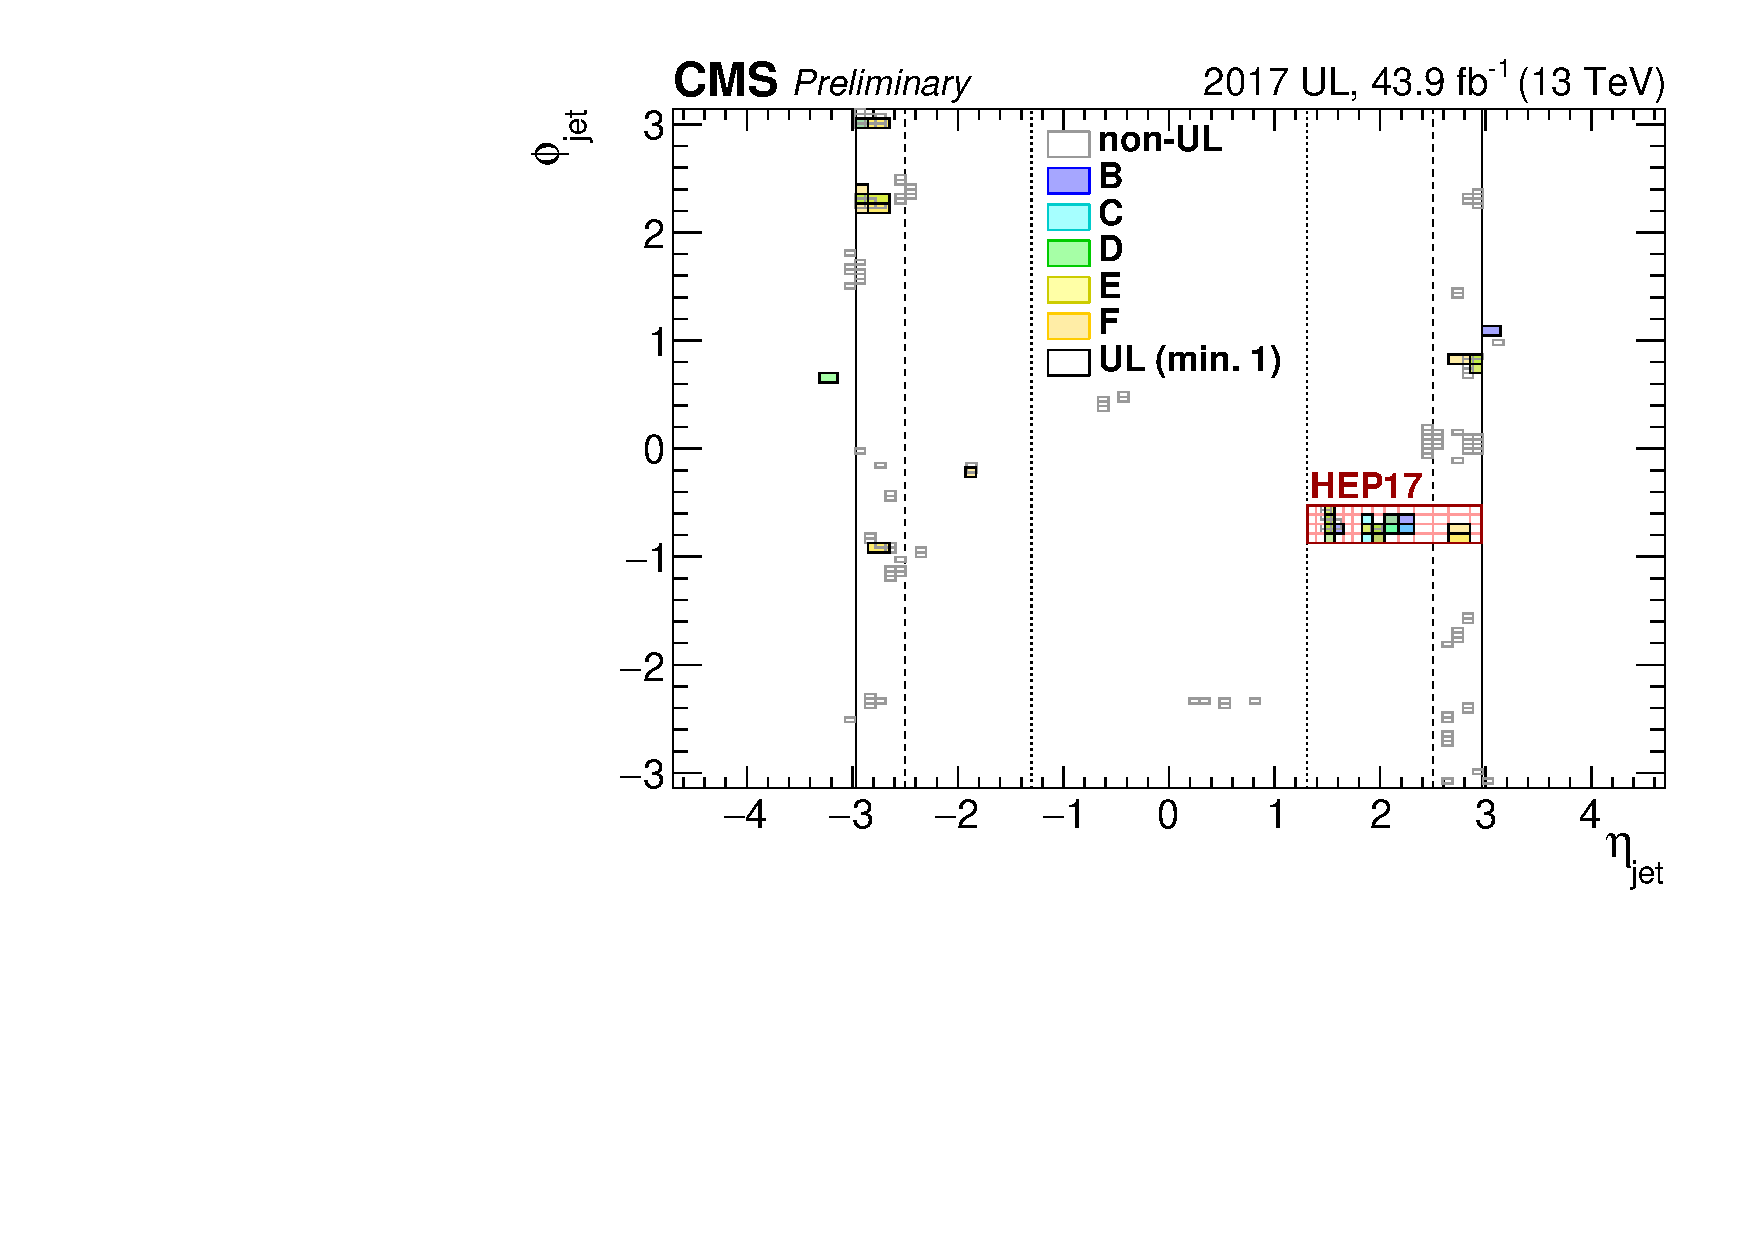
\includegraphics[width=.6\textwidth]{\PhDthesisdir/plots_and_images/hotjets2017UL.pdf}
\caption[Régions des calorimètres à exclure de l'analyse dans le plan $(\eta, \phi)$.]{Régions des calorimètres à exclure de l'analyse dans le plan $(\eta, \phi)$ pour les événements de 2017-UL. Certaines régions ne concernent que certaines périodes de l'année (en couleur). La région \og HEP17 \fg{} correspond à l'emplacement du système de lecture expérimental \og SiPM \fg~\cite{SiPM_CMS_conf}.}
\label{fig-hotjets2017UL}
\end{figure}
%Some regions of the calorimeters are observed to produce anomalously high jet rates. This phenomenon is understood to result from sub-optimal calorimeter calibration for jet measurement performance. We can eliminate any bias arising from the problematic detector regions by excluding events with important jets in the 'hot' calorimeter zones. Hot zone maps are available for the end-of-year (EOY) re-reconstructions for 2016-2018 and the Summer19UL17 reco version in the JECDatabase repository:
%
%https://github.com/cms-jet/JECDatabase/tree/master/hotzone_maps
%
%The EOY maps are there for archiving purposes and we don't have an official recommendation for them at the moment. In the UL17 directory there's two versions; with and without the entire HEP17 HCAL region with sub-optimal calibration resulting from the experimental SiPM read-out system. Our recommendation for UltraLegacy 17 processing is the following:
%
%    All JERC analysers and anybody doing precision measurements with jets should use the h2hot_ul17_plus_hep17 map
%    Searches that are sensitive to jet tails should use h2hot_ul17 for higher acceptance
%    Non-jet measurements and searches that are not sensitive to jet tails can either use h2hot17_ul17 or ignore these maps for highest acceptance
%    Please note that for analyses comparing data to simulation or otherwise relying heavily on simulation, it may be necessary to use the filtering also for MC processing for ensuring avoiding any biases due to angular dependencies etc. In these cases the same data-based filter should be used for data and MC. The maps labelled 'mc' (=pythia) or 'hw' (=herwig) in the JECDatabase are for expert studies only. 
\paragraph{Sélection sur le chemin de déclenchement}
Comme expliqué dans le chapitre~\refChLHCCMS, un événement observé par le détecteur CMS est sauvegardé si un chemin de déclenchement (HLT \emph{path}) est activé.
Dans cette analyse, seuls les événements dont le photon servant d'objet de référence pour la calibration des jets correspond au photon ayant activé le \HLTpath\ pour cet événement sont retenus.
Or, plus l'impulsion transverse du photon est faible, plus le nombre d'événements pouvant être sauvegardés est importante, si bien que la chaîne d'acquisition arrive à saturation.
Pour pallier à cette saturation, il existe différents \HLTpaths\ en fonction de l'impulsion transverse du photon et pour chacun d'entre eux, seule une fraction des événements les déclenchant est effectivement sauvegardée.
Cette fraction est nommée \emph{prescale}.
À chaque \HLTpath\ correspond ainsi un \emph{prescale}.
Un intervalle d'impulsion transverse du photon retenu est alors défini pour chaque \HLTpath\ utilisé.
Cet intervalle permet de se placer au plateau d'efficacité du \HLTpath.
Les différents \HLTpaths, leurs \emph{prescales} et intervalles d'impulsion transverse sont présentés dans le tableau~\ref{tab-HLT_pT_precales_18_and_17UL}.
Par exemple, un photon d'impulsion transverse \SI{95}{\GeV} doit avoir déclenché le chemin nommé \inlinecode{python}{HLT_Photon75_R9Id90_HE10_IsoM}.
\begin{table}[h]
\centering
\begin{tabular}{lccc}
\toprule
\HLTPATH & $\pT^{\photon}$ (\SI{}{\GeV}) & \emph{Prescale} 2018 & \emph{Prescale} 2017-UL\\
\midrule
%\inlinecode{python}{HLT_Photon33} & $[\num{40}, \num{60}[$ & \num{4.0115375867e-5} & \num{3.434860938821936e-4} \\
%\inlinecode{python}{HLT_Photon50_R9Id90_HE10_IsoM} & $[\num{60}, \num{85}[$ & \num{3.9473720141e-3} & \num{7.40465688874224e-3} \\
%\inlinecode{python}{HLT_Photon75_R9Id90_HE10_IsoM} & $[\num{85}, \num{105}[$ & \num{0.0156656382257} & \num{0.03195516364518142} \\
%\inlinecode{python}{HLT_Photon90_R9Id90_HE10_IsoM} & $[\num{105}, \num{130}[$ & \num{0.0312899931745} & \num{0.0636323095006467} \\
%\inlinecode{python}{HLT_Photon120_R9Id90_HE10_IsoM} & $[\num{130}, \num{175}[$ & \num{0.125036122867} & \num{0.18787162142132302} \\
%\inlinecode{python}{HLT_Photon165_R9Id90_HE10_IsoM} & $[\num{175}, \num{230}[$ & \num{0.250030962458} & \num{0.6823580953102895} \\
%\inlinecode{python}{HLT_Photon200} & $[\num{230}, +\infty$ & \num{1} & \num{1} \\
\inlinecode{python}{HLT_Photon33} & $[\num{40}, \num{60}[$ & \num{4.01154e-5} & \num{3.43486e-4} \\
\inlinecode{python}{HLT_Photon50_R9Id90_HE10_IsoM} & $[\num{60}, \num{85}[$ & \num{3.94737e-3} & \num{7.40466e-3} \\
\inlinecode{python}{HLT_Photon75_R9Id90_HE10_IsoM} & $[\num{85}, \num{105}[$ & \num{0.0156656} & \num{0.0319552} \\
\inlinecode{python}{HLT_Photon90_R9Id90_HE10_IsoM} & $[\num{105}, \num{130}[$ & \num{0.0312900} & \num{0.0636323} \\
\inlinecode{python}{HLT_Photon120_R9Id90_HE10_IsoM} & $[\num{130}, \num{175}[$ & \num{0.125036} & \num{0.187872} \\
\inlinecode{python}{HLT_Photon165_R9Id90_HE10_IsoM} & $[\num{175}, \num{230}[$ & \num{0.250031} & \num{0.682358} \\
\inlinecode{python}{HLT_Photon200} & $[\num{230}, +\infty [$ & \num{1} & \num{1} \\
\bottomrule
\end{tabular}
\caption[Chemins de déclenchement.]{\HLTPATHS, intervalles d'impulsion transverse du photon et \emph{prescales} utilisés.}
\label{tab-HLT_pT_precales_18_and_17UL}
\end{table}
\subsection{Analyse}\label{chapter-JERC-section-JES-subsec-analyse}
\paragraph{Intervalles de $\pT^{\photon}$}
L'analyse a pour but de déterminer la correction résiduelle absolue en \pT\ des jets, définie dans la section~\ref{chapter-JERC-section-CMS-subsec-residuals}.
Pour cela, l'écart à l'unité du rapport moyen des réponses des jets dans les données et les simulations est déterminé dans différents intervalles de $\pT^{\photon}$, listés dans le tableau~\ref{tab-pT_photon_intervalles}.
Ils sont une subdivision des intervalles définis pour les \HLTpaths\ dans le tableau~\ref{tab-HLT_pT_precales_18_and_17UL}, ce qui permet de séparer le traitement des événements correspondant à différents \HLTpaths.
\begin{table}[h]
\centering
\begin{tabular}{cccc}
\toprule
$[\num{40}, \num{50}[$ & $[\num{50}, \num{60}[$ & $[\num{60}, \num{85}[$ & $[\num{85}, \num{105}[$ \\
$[\num{105}, \num{130}[$ & $[\num{130}, \num{175}[$ & $[\num{175}, \num{230}[$ & $[\num{230}, \num{300}[$ \\
$[\num{300}, \num{400}[$ & $[\num{400}, \num{500}[$ & $[\num{500}, \num{700}[$ & $[\num{700}, \num{1000}[$ \\
$[\num{1000}, \num{3000}]$ \\
\bottomrule
\end{tabular}
\caption[Intervalles de $\pT^{\photon}$.]{Intervalles de $\pT^{\photon}$ en \SI{}{\GeV}.}
\label{tab-pT_photon_intervalles}
\end{table}
\paragraph{Intervalles de $\abs{\eta^\text{jet}}$}
La calibration en énergie des jets dépend fortement de la région du détecteur dans laquelle le jet laisse un signal, comme le montre la figure~\ref{fig-simulated_jet_response_RunII} en page~\pageref{fig-simulated_jet_response_RunII}.
Cet effet est dû aux différentes technologies utilisées ainsi qu'au vieillissement non uniforme du détecteur.
Des intervalles de pseudo-rapidité du jet sont ainsi définis dans le tableau~\ref{tab-eta_jet_intervalles_large} afin de séparer le traitement de ces différentes régions.
\begin{table}[h]
\centering
\begin{tabular}{cccc}
\toprule
$[\num{0}\isp \num{0.783}[$ & $[\num{0.783}\isp \num{1.305}[$ & $[\num{1.305}\isp \num{1.93}[$ & $[\num{1.93}\isp \num{2.5}[$ \\
$[\num{2.5}\isp \num{2.964}[$ & $[\num{2.964}\isp \num{3.2}[$ & $[\num{3.2}\isp \num{5.191}[$ &  \\
\bottomrule
\end{tabular}
\caption{Intervalles larges de $\abs{\eta^\text{jet}}$.}
\label{tab-eta_jet_intervalles_large}
\end{table}
%\begin{table}[h]
%\centering
%\begin{tabular}{cccccc}
%\toprule
%$[\num{0}\isp \num{0.261}[$ & $[\num{0.261}\isp \num{0.522}[$ & $[\num{0.522}\isp \num{0.783}[$ & $[\num{0.783}\isp \num{1.044}[$ & $[\num{1.044}\isp \num{1.305}[$ & $[\num{1.305}\isp \num{1.479}[$ \\
%$[\num{1.479}\isp \num{1.653}[$ & $[\num{1.653}\isp \num{1.930}[$ & $[\num{1.930}\isp \num{2.172}[$ & $[\num{2.172}\isp \num{2.322}[$ & $[\num{2.322}\isp \num{2.500}[$ & $[\num{2.500}\isp \num{2.650}[$ \\
%$[\num{2.650}\isp \num{2.853}[$ & $[\num{2.853}\isp \num{2.964}[$ & $[\num{2.964}\isp \num{3.319}[$ & $[\num{3.319}\isp \num{3.489}[$ & $[\num{3.489}\isp \num{3.839}[$ & $[\num{3.839}\isp \num{5.191}[$ \\
%\bottomrule
%\end{tabular}
%\caption{Intervalles fins de $\abs{\eta^\text{jet}}$.}
%\label{tab-eta_jet_intervalles_fin}
%\end{table}
\paragraph{Pondération par l'empilement}
Le profil d'empilement, \ie\ la densité de probabilité du nombre d'interactions d'empilement, dépend de la période de la prise de données et du \HLTpath\ par lequel l'événement est retenu. Ces dépendances sont illustrées sur les graphiques des figures~\ref{fig-PU_profile_18} et~\ref{fig-PU_profile_17UL}.
Les événements simulés sont ainsi pondérés pour faire correspondre leur profil d'empilement à celui des données, en prenant en compte la double dépendance avec la période de prise de donnée et le \HLTpath.
\begin{figure}[p]
\centering
\subcaptionbox{Run 2018 A.\label{subfig-PU_profile_18_A}}[.45\textwidth]
{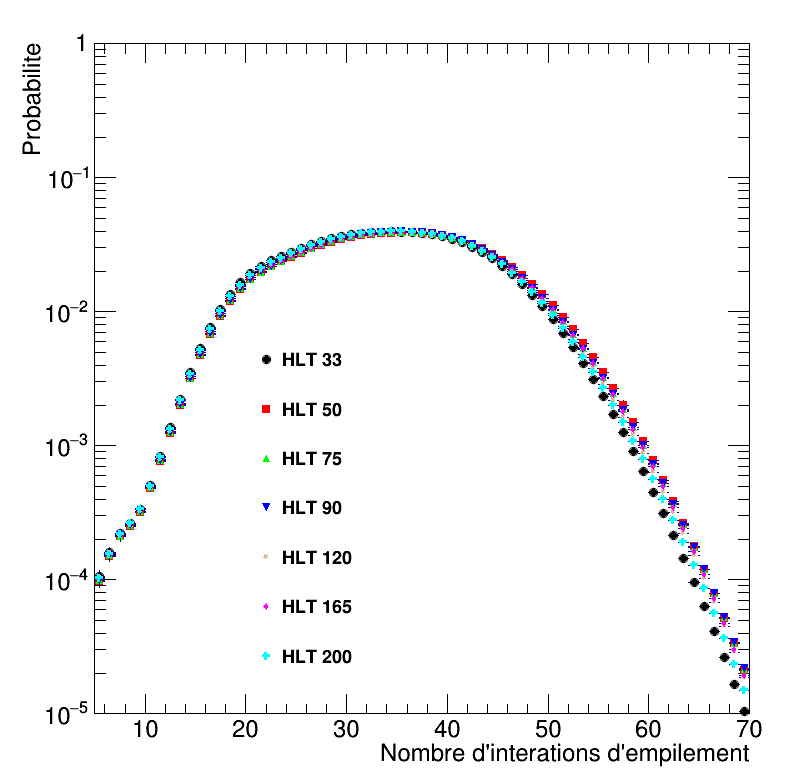
\includegraphics[width=.45\textwidth]{\PhDthesisdir/plots_and_images/my_plots/JERC/PUreweighting/2018/with_header/PU_HLT_profiles_run2018A_only_L2Res.tex}\vspace{-.5\baselineskip}}
\hfill
\subcaptionbox{Run 2018 B.\label{subfig-PU_profile_18_B}}[.45\textwidth]
{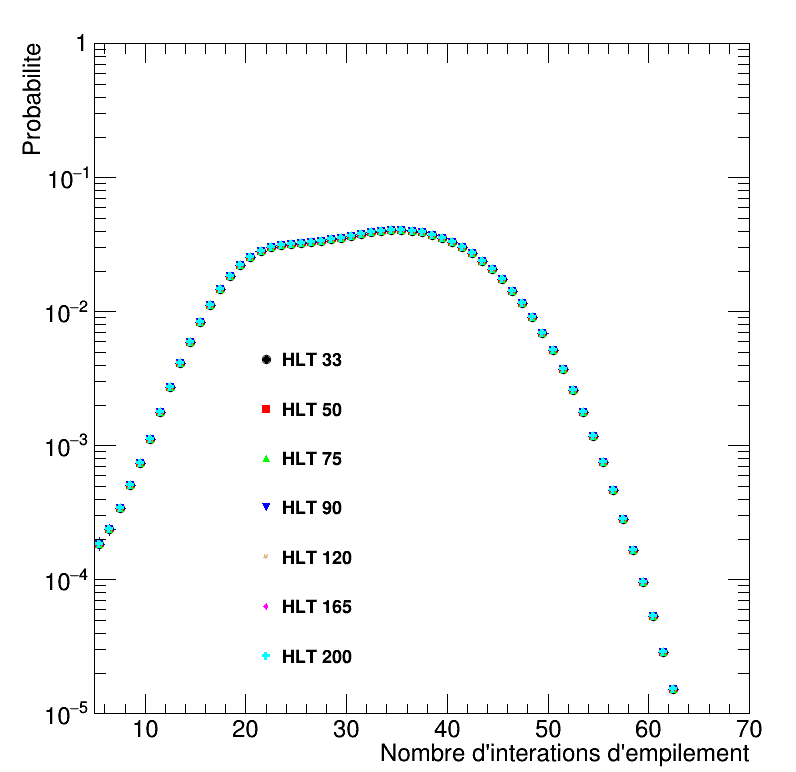
\includegraphics[width=.45\textwidth]{\PhDthesisdir/plots_and_images/my_plots/JERC/PUreweighting/2018/with_header/PU_HLT_profiles_run2018B_only_L2Res.tex}\vspace{-.5\baselineskip}}

\vspace{.75\baselineskip}

\subcaptionbox{Run 2018 C.\label{subfig-PU_profile_18_C}}[.45\textwidth]
{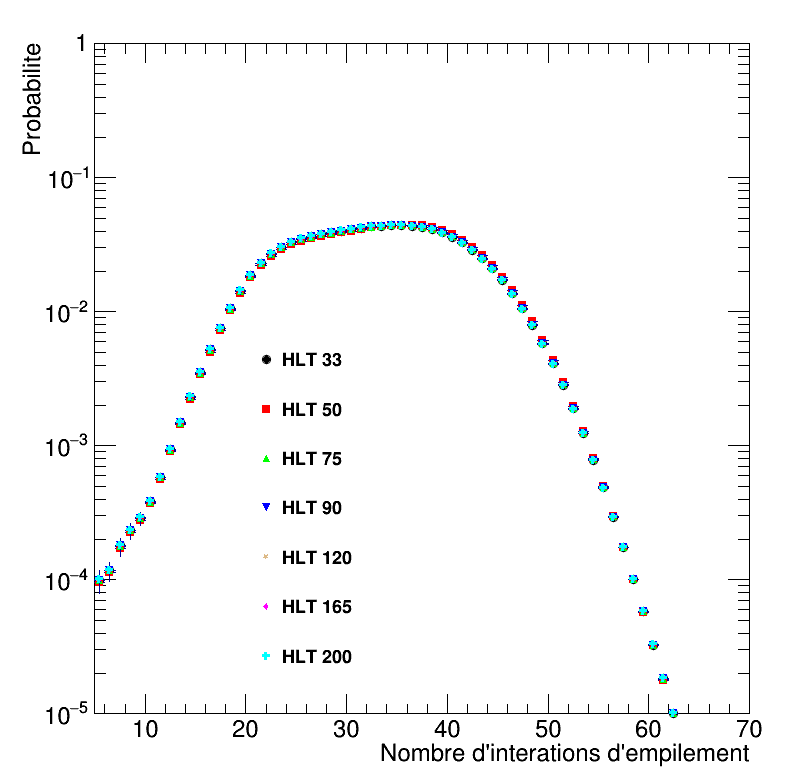
\includegraphics[width=.45\textwidth]{\PhDthesisdir/plots_and_images/my_plots/JERC/PUreweighting/2018/with_header/PU_HLT_profiles_run2018C_only_L2Res.tex}\vspace{-.5\baselineskip}}
\hfill
\subcaptionbox{Run 2018 D.\label{subfig-PU_profile_18_D}}[.45\textwidth]
{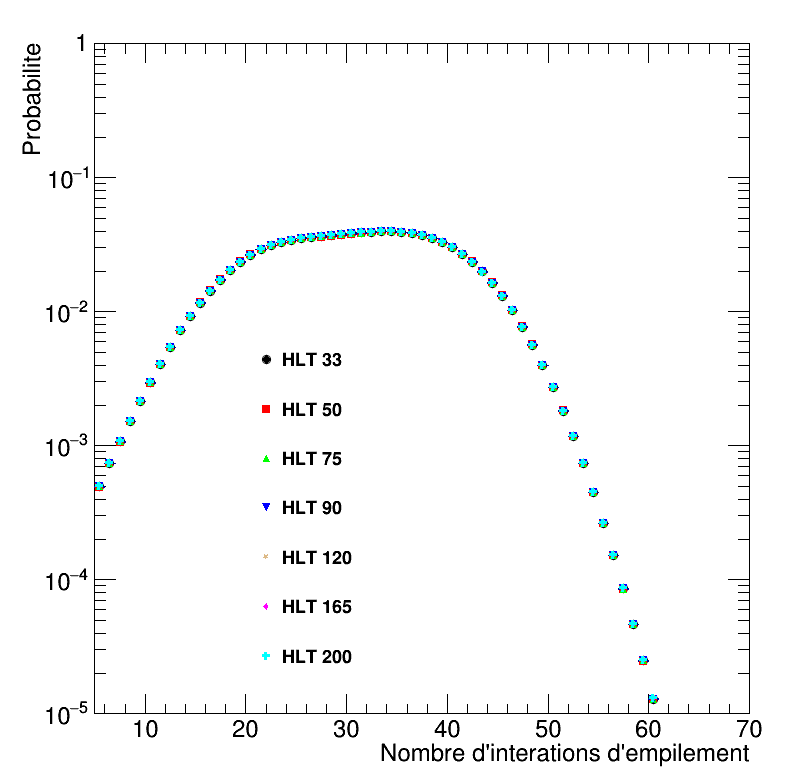
\includegraphics[width=.45\textwidth]{\PhDthesisdir/plots_and_images/my_plots/JERC/PUreweighting/2018/with_header/PU_HLT_profiles_run2018D_only_L2Res.tex}\vspace{-.5\baselineskip}}

\vspace{.75\baselineskip}

\subcaptionbox{Run 2018 ABC.\label{subfig-PU_profile_18_ABC}}[.45\textwidth]
{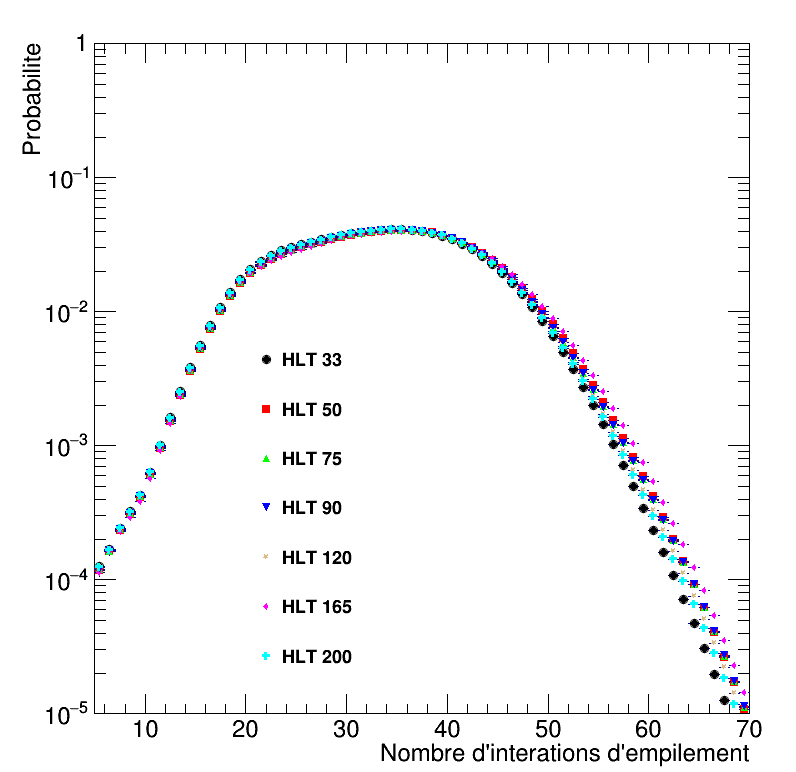
\includegraphics[width=.45\textwidth]{\PhDthesisdir/plots_and_images/my_plots/JERC/PUreweighting/2018/with_header/PU_HLT_profiles_run2018ABC_only_L2Res.tex}\vspace{-.5\baselineskip}}
\hfill
\subcaptionbox{Run 2018 ABCD.\label{subfig-PU_profile_18_ABCD}}[.45\textwidth]
{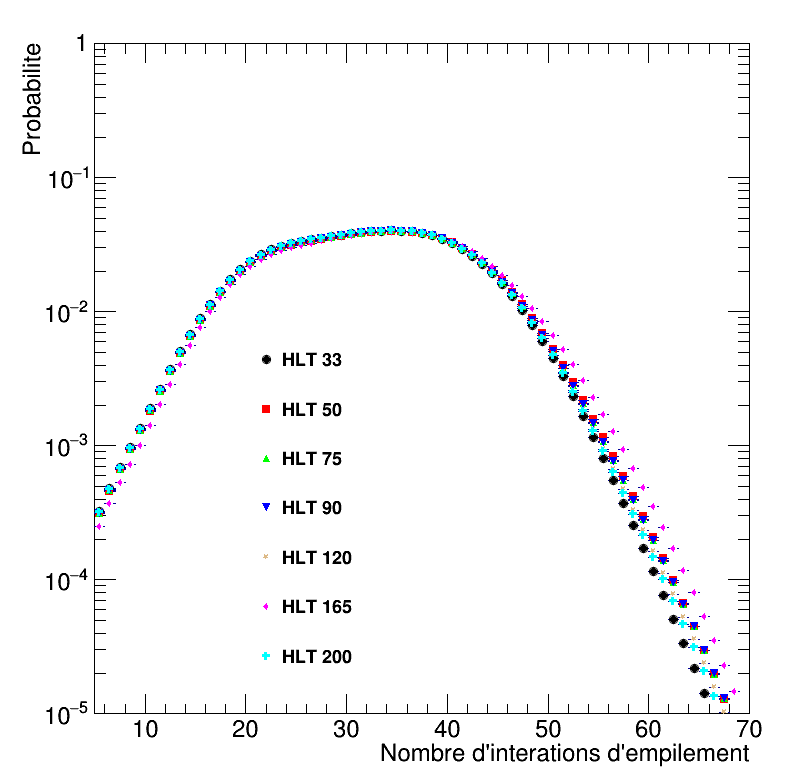
\includegraphics[width=.45\textwidth]{\PhDthesisdir/plots_and_images/my_plots/JERC/PUreweighting/2018/with_header/PU_HLT_profiles_run2018ABCD_only_L2Res.tex}\vspace{-.5\baselineskip}}

\caption[Densités de probabilité de $N_\text{PU}$ pour 2018.]{Densités de probabilité du nombre d'interactions d'empilement $N_\text{PU}$ pour les périodes de prises de données de 2018.}
\label{fig-PU_profile_18}
\end{figure}
\begin{figure}[p]
\centering
\subcaptionbox{Run 2017-UL B.\label{subfig-PU_profile_17UL_B}}[.45\textwidth]
{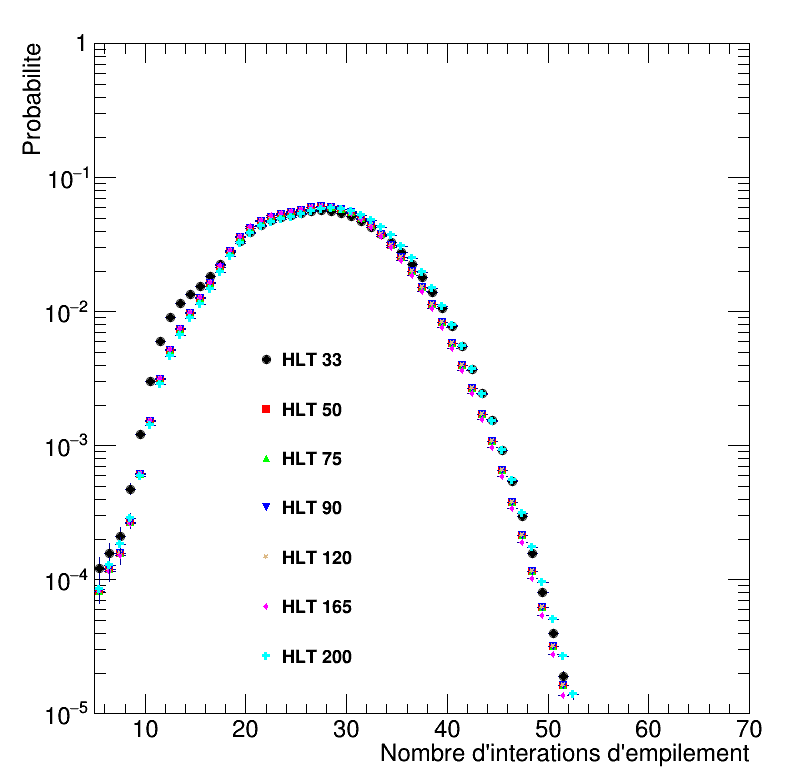
\includegraphics[width=.45\textwidth]{\PhDthesisdir/plots_and_images/my_plots/JERC/PUreweighting/2017UL/with_header/PU_HLT_profiles_run2017B_only_L2Res.tex}\vspace{-.5\baselineskip}}
\hfill
\subcaptionbox{Run 2017-UL C.\label{subfig-PU_profile_17UL_C}}[.45\textwidth]
{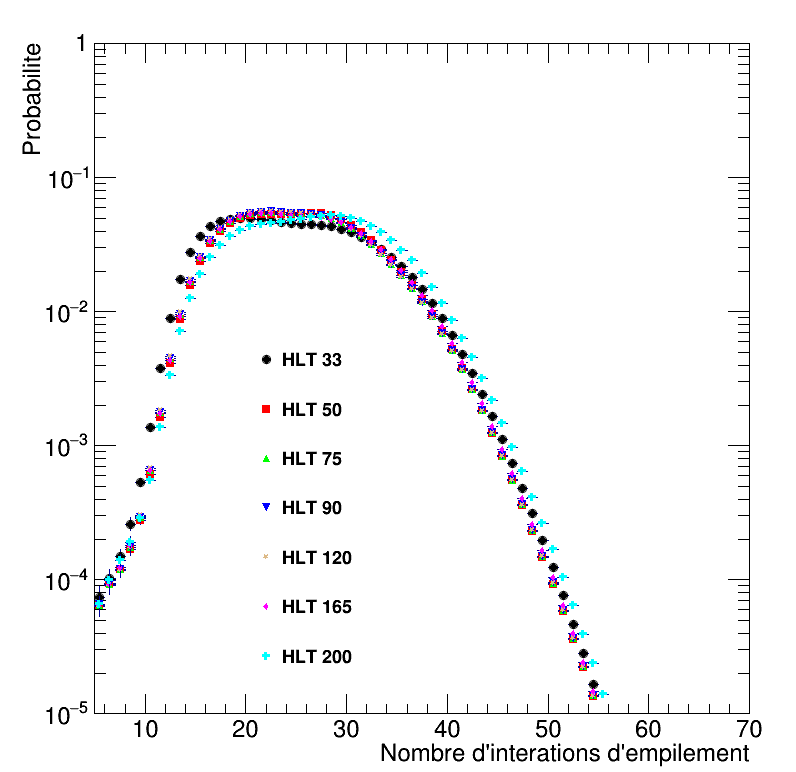
\includegraphics[width=.45\textwidth]{\PhDthesisdir/plots_and_images/my_plots/JERC/PUreweighting/2017UL/with_header/PU_HLT_profiles_run2017C_only_L2Res.tex}\vspace{-.5\baselineskip}}

\vspace{.75\baselineskip}

\subcaptionbox{Run 2017-UL D.\label{subfig-PU_profile_17UL_D}}[.45\textwidth]
{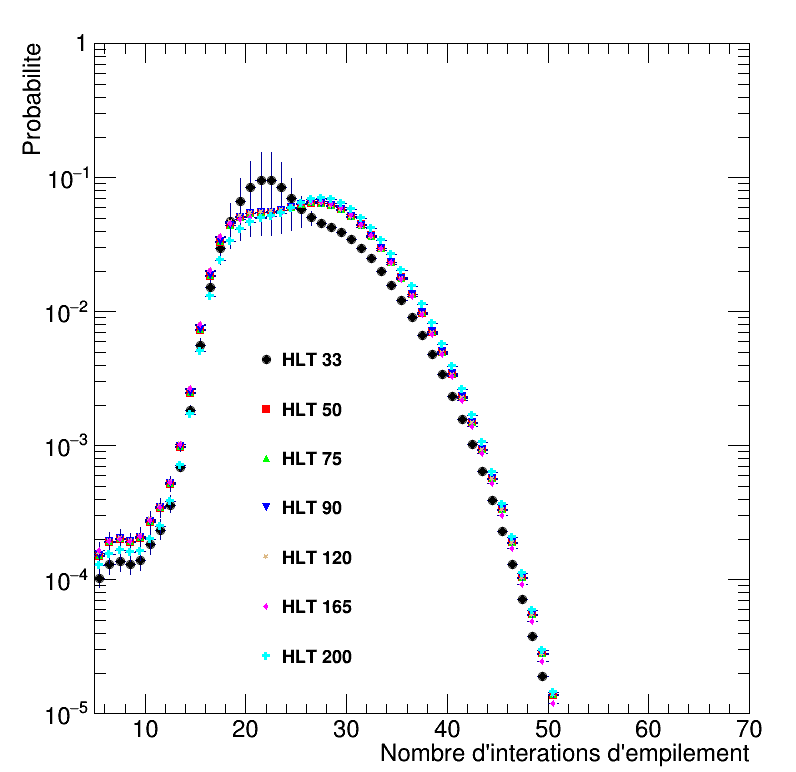
\includegraphics[width=.45\textwidth]{\PhDthesisdir/plots_and_images/my_plots/JERC/PUreweighting/2017UL/with_header/PU_HLT_profiles_run2017D_only_L2Res.tex}\vspace{-.5\baselineskip}}
\hfill
\subcaptionbox{Run 2017-UL E.\label{subfig-PU_profile_17UL_E}}[.45\textwidth]
{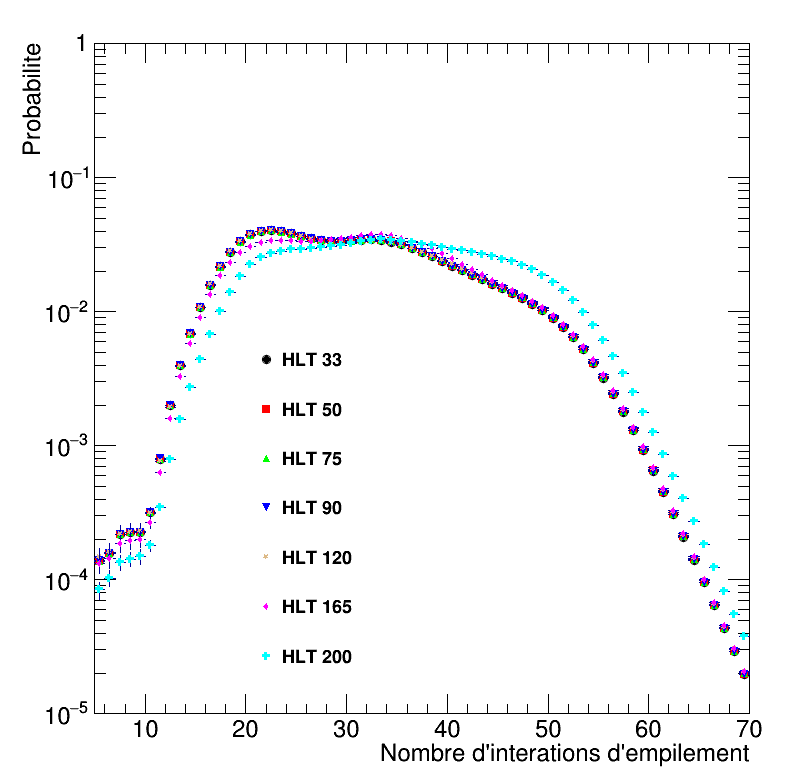
\includegraphics[width=.45\textwidth]{\PhDthesisdir/plots_and_images/my_plots/JERC/PUreweighting/2017UL/with_header/PU_HLT_profiles_run2017E_only_L2Res.tex}\vspace{-.5\baselineskip}}

\vspace{.75\baselineskip}

\subcaptionbox{Run 2017-UL F.\label{subfig-PU_profile_17UL_F}}[.45\textwidth]
{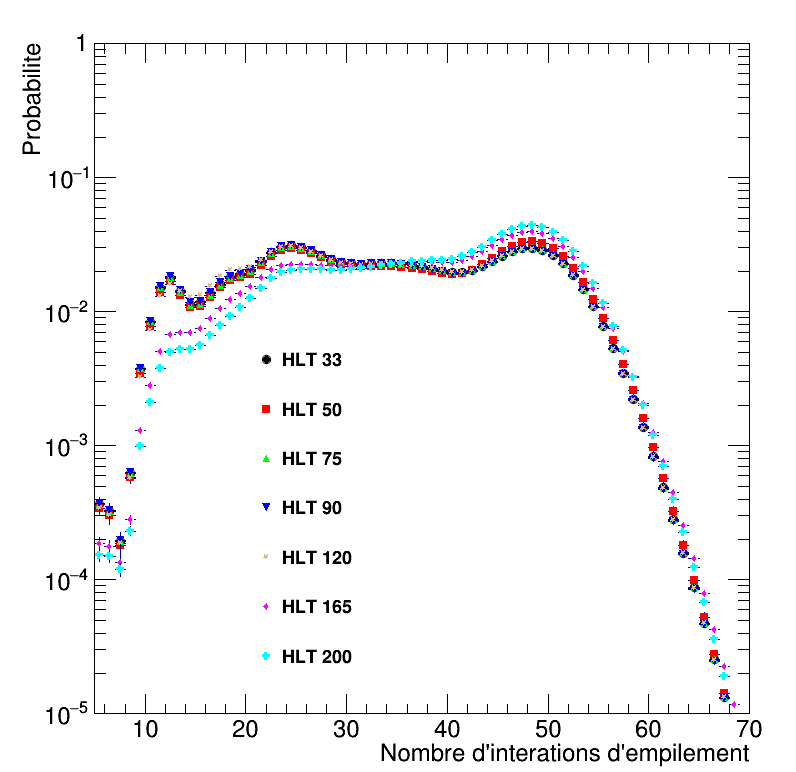
\includegraphics[width=.45\textwidth]{\PhDthesisdir/plots_and_images/my_plots/JERC/PUreweighting/2017UL/with_header/PU_HLT_profiles_run2017F_only_L2Res.tex}\vspace{-.5\baselineskip}}
\hfill
\subcaptionbox{Run 2017-UL BCDEF.\label{subfig-PU_profile_17UL_BCDEF}}[.45\textwidth]
{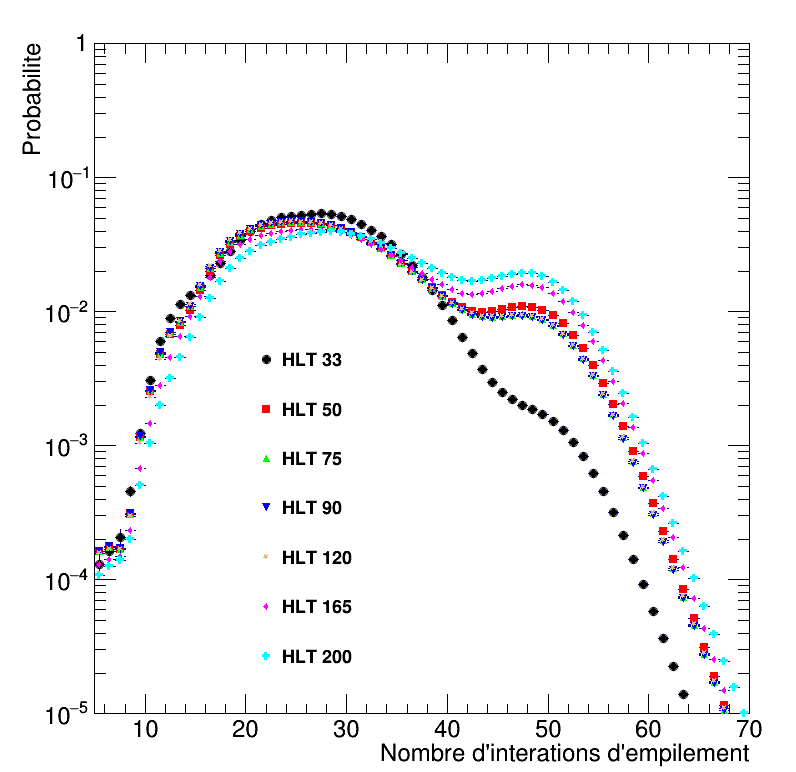
\includegraphics[width=.45\textwidth]{\PhDthesisdir/plots_and_images/my_plots/JERC/PUreweighting/2017UL/with_header/PU_HLT_profiles_run2017BCDEF_only_L2Res.tex}\vspace{-.5\baselineskip}}

\caption[Densités de probabilité de $N_\text{PU}$ pour 2017-UL.]{Densités de probabilité du nombre d'interactions d'empilement $N_\text{PU}$ pour les périodes de prises de données de 2017-UL.}
\label{fig-PU_profile_17UL}
\end{figure}
\paragraph{Accord données-simulations}
Pour comparer les distributions des observables dans les événements, les distributions des événements simulés sont normalisées à la luminosité mesurée pour le jeu de données considéré.
Les comparaisons étant faites entre les données et les événements simulés \Gjets, un désaccord dû à la contamination à bas \pT\ d'événements multijet est attendu, ces événements n'étant pas présents dans les simulations utilisées.
De plus, l'utilisation d'une simulation au premier ordre perturbatif seulement influe sur le nombre de jets dans l'état final qui s'en trouve plus faible, en particulier dans les queues des distributions.
Ces désaccords se constatent sur les graphiques de la figure~\ref{fig-distribs_Gjets_18} présentant les distributions de l'impulsion transverse du photon, l'énergie transverse manquante et les impulsions transverses du premier et du second jet.
Afin de déterminer la correction résiduelle absolue en \pT\ des jets ainsi que la correction de leur résolution en énergie, seule la comparaison des distributions de \Rbal\ et \RMPF\ est nécessaire.
L'accord ainsi obtenu entre données et simulations est considéré comme suffisant.
\begin{figure}[h]
\centering
\subcaptionbox{Impulsion transverse du photon.\label{subfig-distrib_Gjets_18_ptPhoton}}[.45\textwidth]
{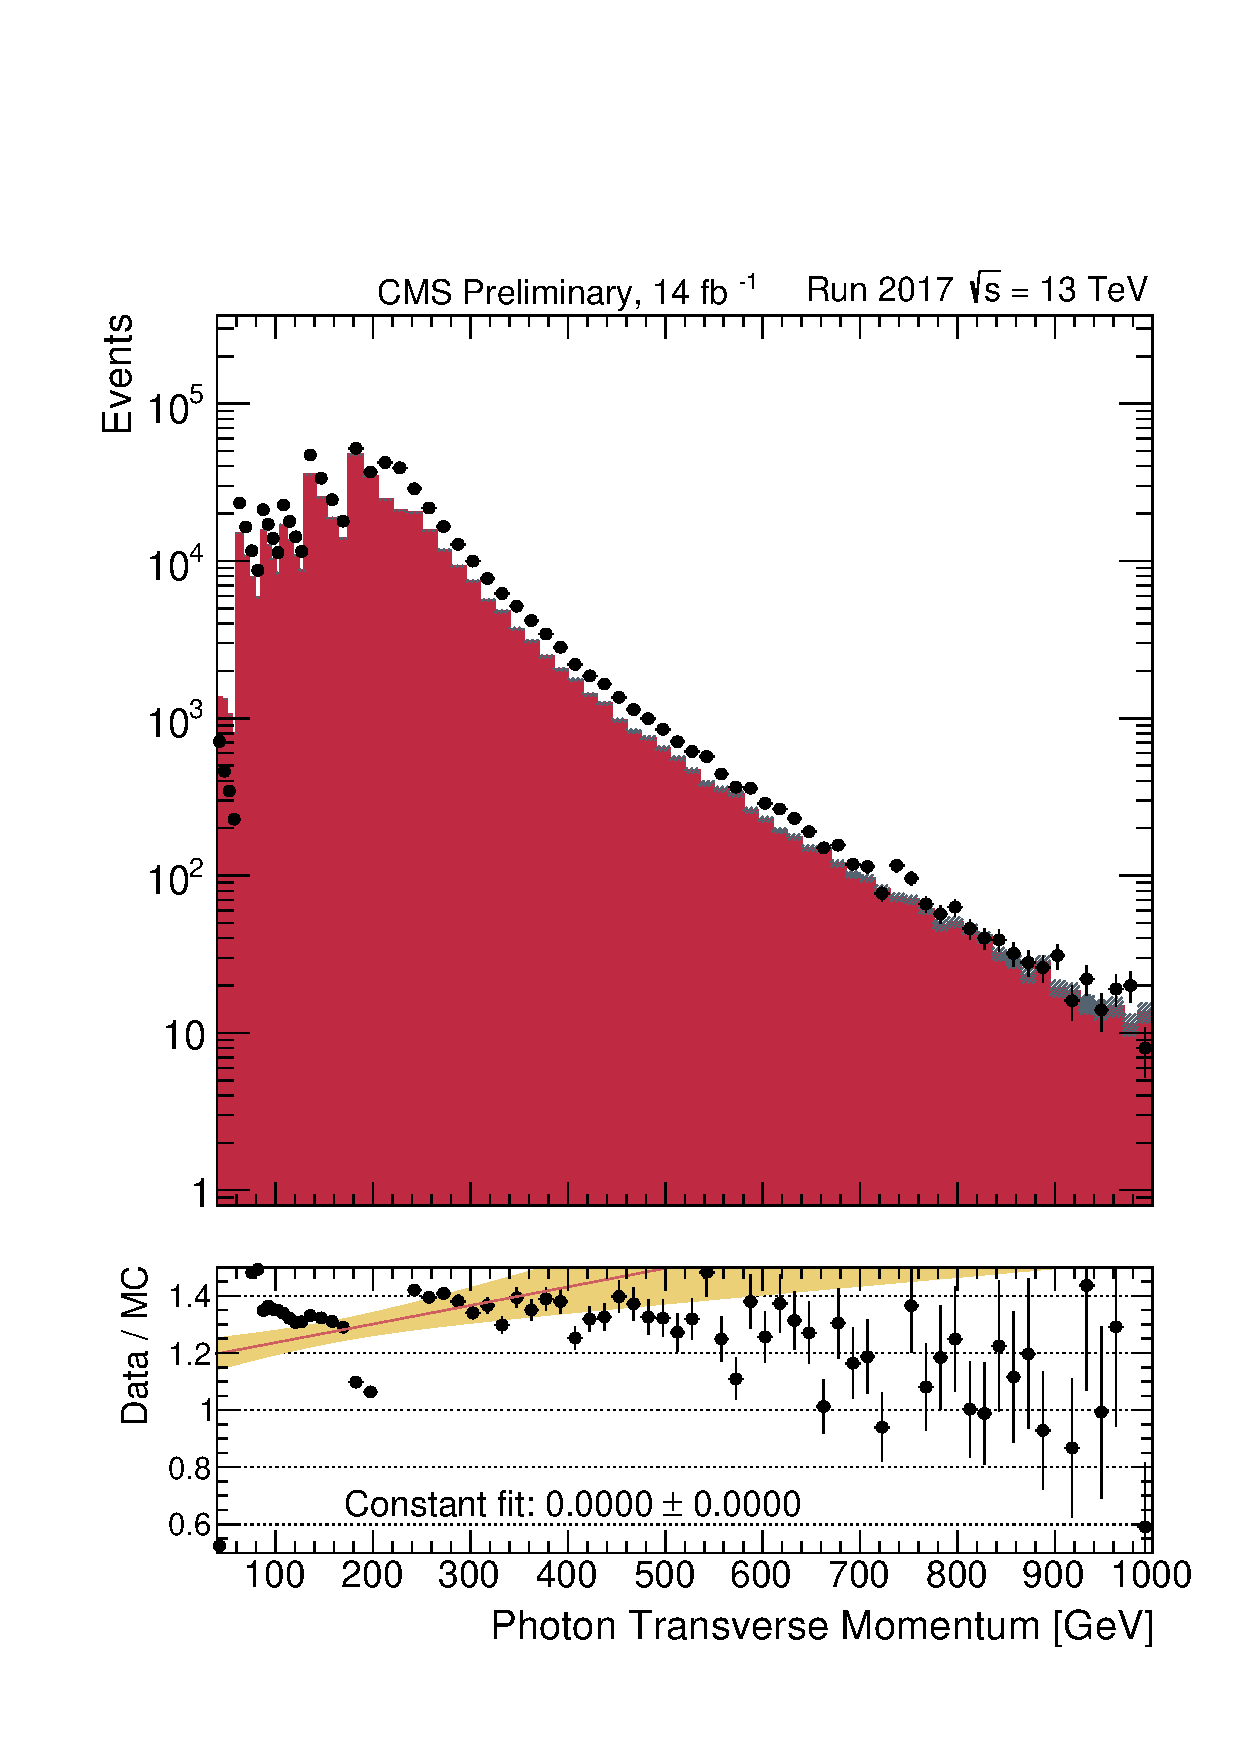
\includegraphics[width=.45\textwidth]{\PhDthesisdir/plots_and_images/my_plots/JERC/distributions/2018/with_header/ptPhoton_log.tex}}
\hfill
\subcaptionbox{Énergie transverse manquante.\label{subfig-distrib_Gjets_18_MET}}[.45\textwidth]
{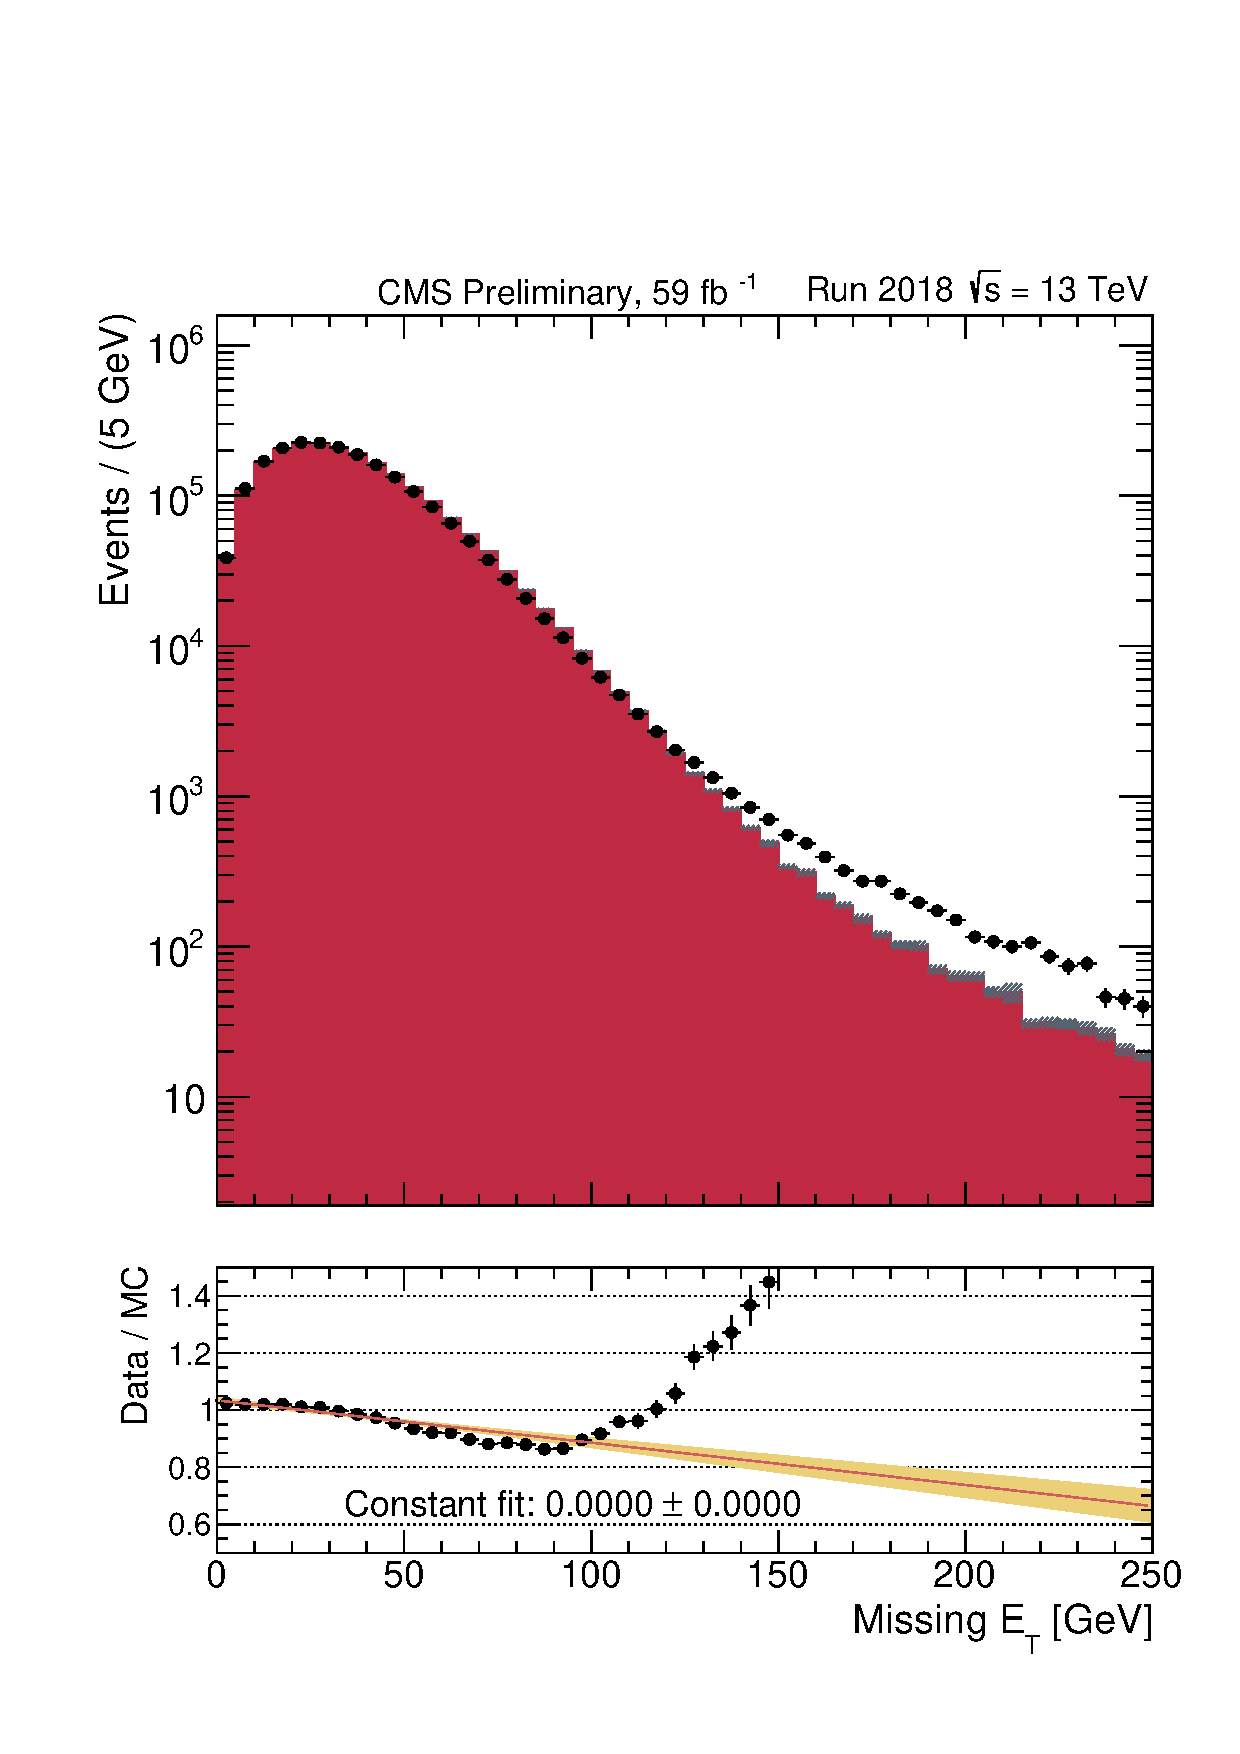
\includegraphics[width=.45\textwidth]{\PhDthesisdir/plots_and_images/my_plots/JERC/distributions/2018/with_header/MET_log.tex}}

\vspace{\baselineskip}

\subcaptionbox{Impulsion transverse du premier jet.\label{subfig-distrib_Gjets_18_ptFirstJet}}[.45\textwidth]
{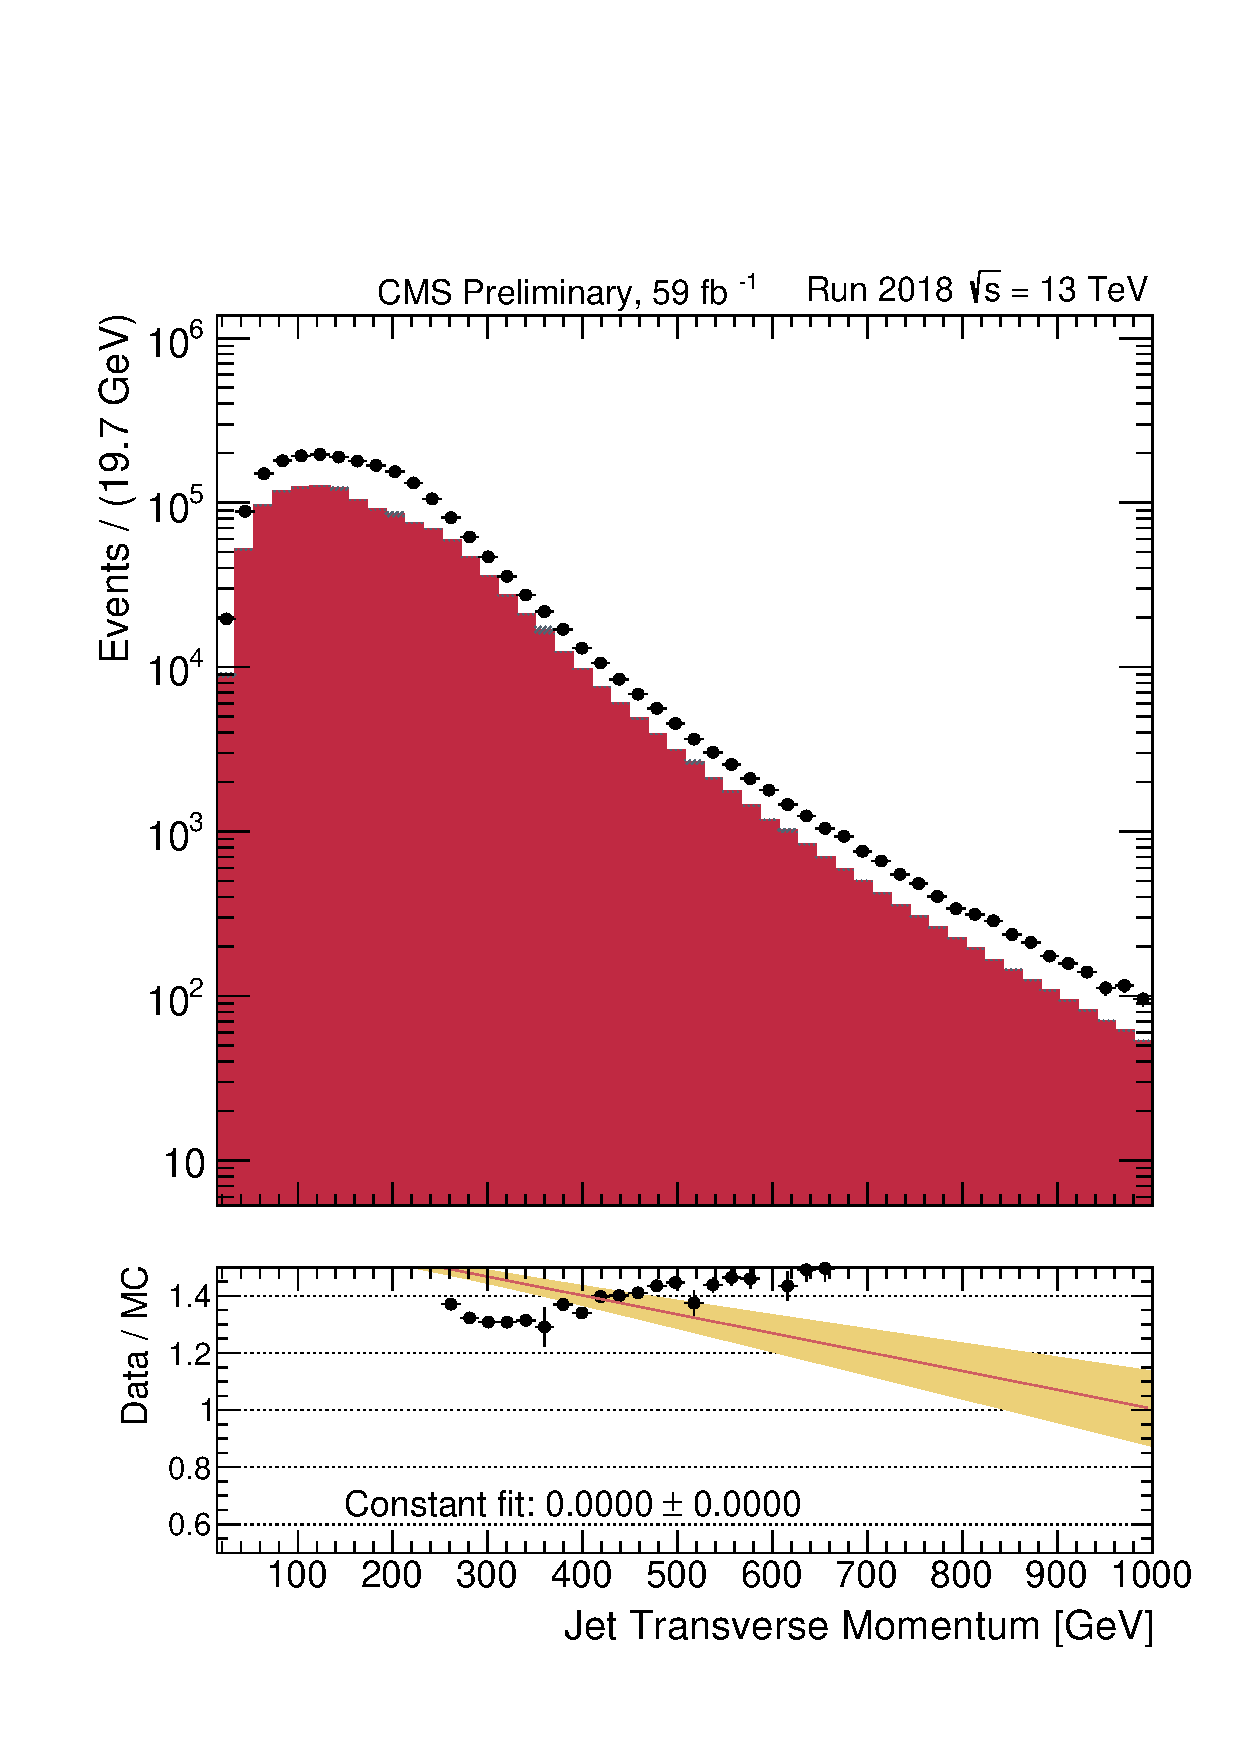
\includegraphics[width=.45\textwidth]{\PhDthesisdir/plots_and_images/my_plots/JERC/distributions/2018/with_header/ptFirstJet_log.tex}}
\hfill
\subcaptionbox{Impulsion transverse du second jet.\label{subfig-distrib_Gjets_18_ptSecondJet}}[.45\textwidth]
{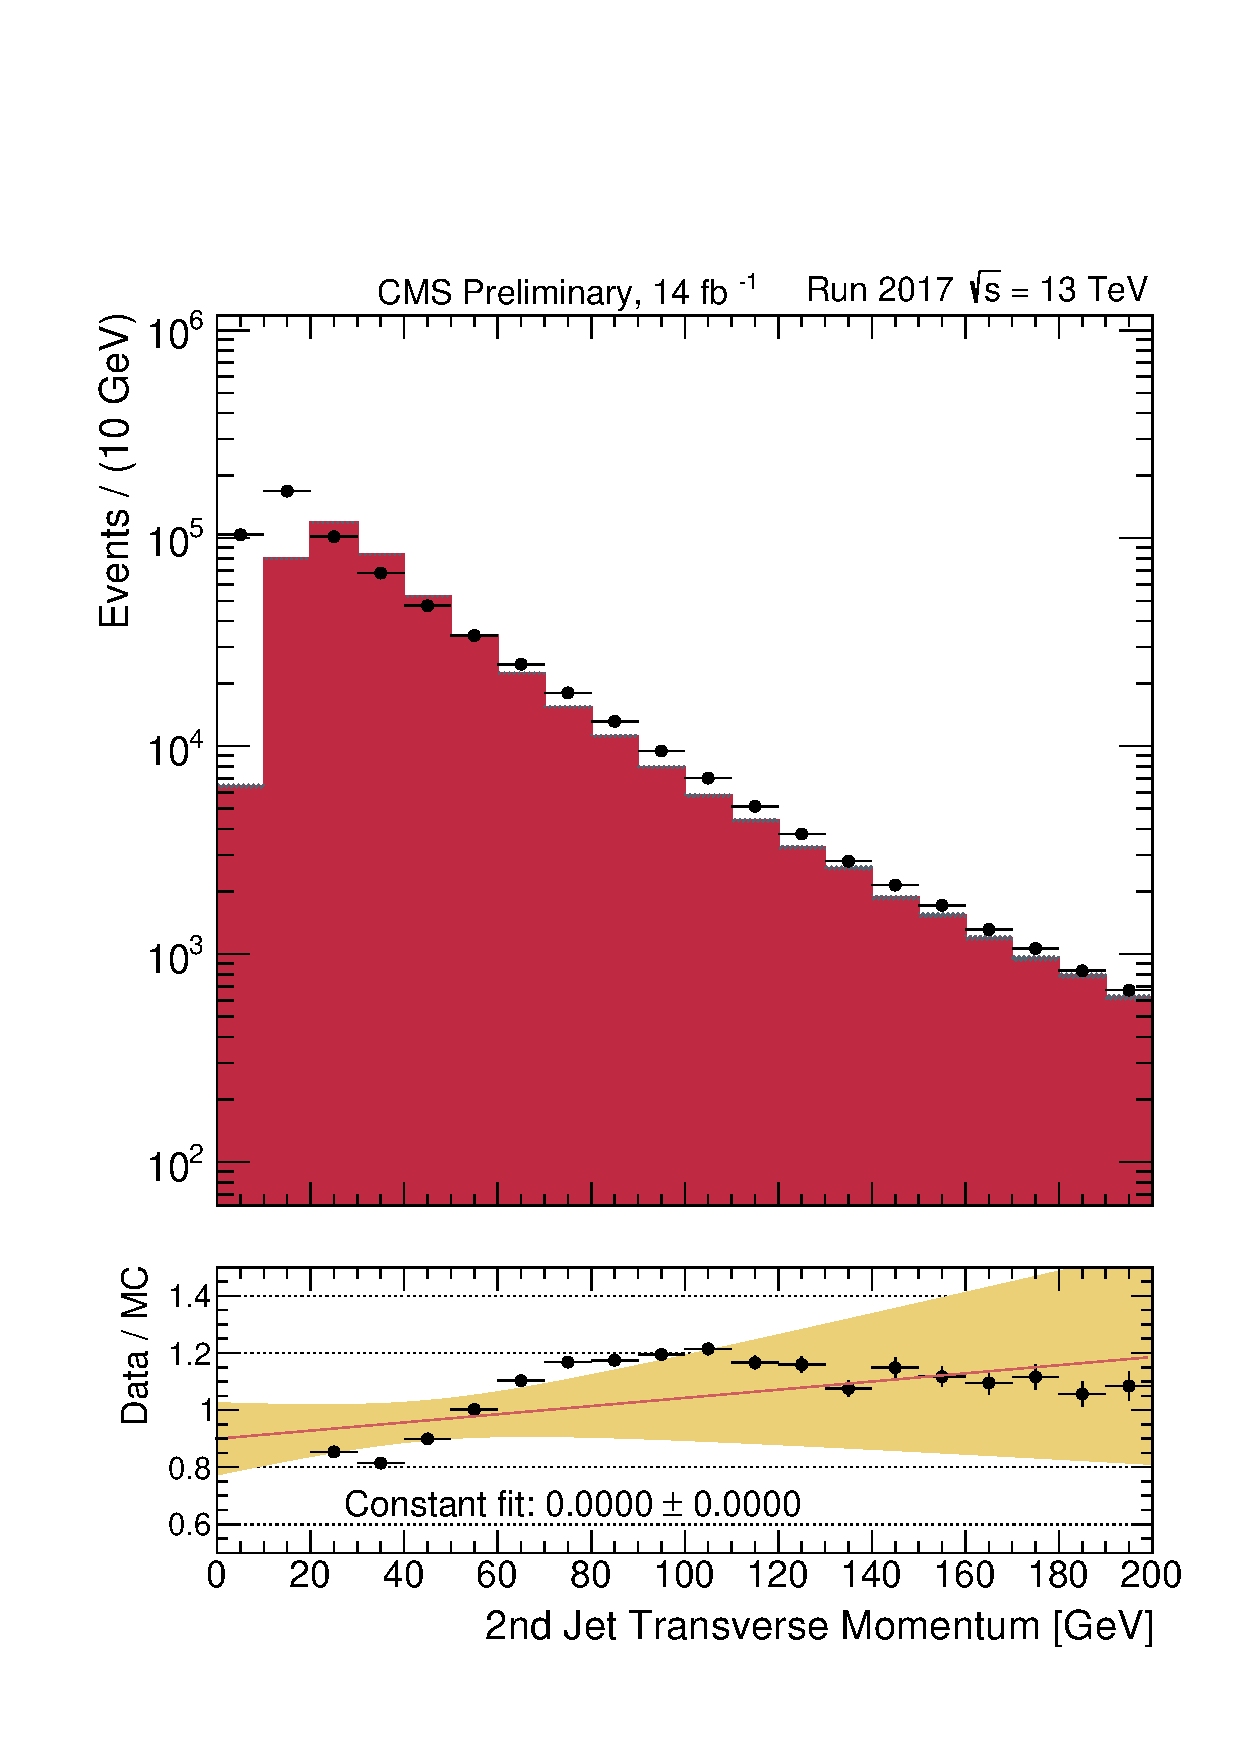
\includegraphics[width=.45\textwidth]{\PhDthesisdir/plots_and_images/my_plots/JERC/distributions/2018/with_header/ptSecondJet_log.tex}}

\caption[Observables d'événements \Gjets\ en 2018.]{Distributions d'observables dans les données (points noirs) et les simulations (histogramme en rouge) pour l'année 2018. Sur la figure~\ref{subfig-distrib_Gjets_18_ptPhoton}, l'effet des \emph{prescales} (voir page~\pageref{tab-HLT_pT_precales_18_and_17UL}) donnant une distribution en dents de scie est clairement visible.}
\label{fig-distribs_Gjets_18}
\end{figure}
\paragraph{Activité additionnelle des jets supplémentaires}
La présence d'un jet secondaire, comme sur la figure~\ref{subfig-Gamma_plus_two_jets}, créé un déséquilibre dans \Rbal\ dû à la physique de l'événement et non à la JES. Il ne faut donc pas corriger cet effet.
Pour cela, il faut pouvoir se ramener au cas où un seul jet est présent, comme dans l'événement de la figure~\ref{subfig-Gamma_plus_jet_basic_event}.
L'activité additionnelle liée aux jets supplémentaires est quantifiée par la variable
\begin{equation}
\alpha = \frac{\pT_\reco^\text{jet 2}}{\pT^{\photon}}
\mend
\label{eq-chapter-JERC-definition_alpha}
\end{equation}
\par L'analyse des événements \Gjets\ est alors réalisée pour différents intervalles de $\alpha$ afin de pouvoir réaliser par la suite une extrapolation à $\alpha=0$, correspondant au cas idéal d'événements \Gjet.
Les intervalles utilisés sont présentés dans le tableau~\ref{tab-alpha_intervalles}.
Il s'agit d'intervalles inclusifs, \ie\ que chaque intervalle contient l'intervalle précédent.
L'évolution des réponses moyennes en fonction de $\alpha$ y étant linéaire \aposteriori, ce qui se retrouve dans les résultats de la figure~\ref{fig-chapter-JERC-section-JES-subsec-analyse-responsebal_and_MPF_eta0013_ptPhot_175_230_extrap}, page~\pageref{fig-chapter-JERC-section-JES-subsec-analyse-responsebal_and_MPF_eta0013_ptPhot_175_230_extrap}, ce choix rend possible une extrapolation simple vers $\alpha=0$.
\begin{table}[h]
\centering
\begin{tabular}{ccccc}
\toprule
$[\num{0}\isp \num{0.10}[$ & $[\num{0}\isp \num{0.15}[$ & $[\num{0}\isp \num{0.20}[$ & $[\num{0}\isp \num{0.25}[$ & $[\num{0}\isp \num{0.30}[$ \\
\bottomrule
\end{tabular}
\caption{Intervalles de $\alpha$ utilisés pour la JES.}
\label{tab-alpha_intervalles}
\end{table}
\par Des études sont en cours afin d'inclure des valeurs de $\alpha$ allant jusqu'à \num{1}.
L'exploitation des événements tels que $\alpha>\num{0.3}$ est doublement motivée.
Ces événements permettraient d'améliorer les corrections vis-à-vis du FSR introduit page~\pageref{subfig-fgraph-gq_qGamma_S-FSR_2jets} et les corrections à bas \pT.
En effet, pour $\pT^{\photon}<\SI{100}{\GeV}$, imposer $\alpha<\num{0.3}$ implique $\pT^\text{jet 2}<\SI{30}{\GeV}$, ce qui limite fortement le nombre d'événements exploitables.
%Mikko:
%The alpha>0.3 values are not (yet) used to constrain the FSR correction because they are outside the linear regime, but I’m working on including them for better low pT constraints. It’s a new unexplored region so taking some time to understand to sufficient detail.
%The alpha values higher than 0.3 may be necessary for reliably extending the measurement below pT<100 GeV. Here alpha<0.3 corresponds to pT2=30 GeV, which is the threshold below which pileup jet rates start to rapidly increase. This leads to large alpha cut inefficiencies and strong bias on average <rho> (i.e. PU profile). So the best solution might be to have a sliding cut of alpha<30 GeV/pT,gamma at pT<100 GeV instead of fixed 0.3.
%On the other hand, I know that dR/dalpha is quite linear at alpha<0.3 so initially I was thinking that having steps of fixed values of alpha could work, where alphamax > 30 GeV/pTZ. There are topological boundaries like ~0.35, where the second jet is almost the same pT as leading jet, if both opposite to Z. For values alpha>0.5 the second jet usually has to be opposite to the leading jet and on the same side as Z (as DeltaPhi forces it to be either parallel or antiparallel, unless it’s a three jet event). This make dR/dalpha flatten out at ~0.35-0.5 and then change sign at alpha>0.5.
%So from the initial Z+jet studies in Helsinki it seems like thresholds of alpha<0.5 (safe down to pT=60 GeV) and alpha<1.0 (safe down to pT=30 GeV) could be quite useful for low pT. The MPF method in particular is still robust for these values, and we actually have <pT1>/<pTZ> close to unity than for alpha<0.3, which has essentially maximised the difference in <pT1> and <pTZ>.
%I’ve not yet activated alpha<0.5 and 1.0 because they are missing from the official Z+jet inputs from KIT (I only have them in our Helsinki study, which is in other respects less advanced than the KIT one). I also foresee needing the unclustered energy and secondary jet sum estimates for properly correcting MPF without extrapolated FSR correction in the non-linear regime.
\paragraph{Obtention des corrections pour $\pT^{\photon}, \eta^\text{jet}, (\alpha^\text{max})$ donnés}
Pour chaque domaine
de $\pT^{\photon}$ défini dans le tableau~\ref{tab-pT_photon_intervalles},
de $\eta^\text{jet}$ défini dans le tableau~\ref{tab-eta_jet_intervalles_large} et
de $\alpha$ défini dans le tableau~\ref{tab-alpha_intervalles},
les distributions des réponses balancée et MPF des données et des simulations sont déterminées.
Certaines de ces distributions sont représentées sur la figure~\ref{fig-distribs_Gjets_18_resp_bal_and_mpf}.
\par Afin de limiter les effets des queues de ces distributions, en particulier dans le cas de la réponse balancée,
une troncature leur est appliquée pour n'en conserver que les parties centrales.
Pour cela, un ajustement à une gaussienne est réalisé pour chaque distribution.
Les points considérés dans la suite sont alors ceux appartenant à un intervalle  $[ \bar{R} - \Delta R, \bar{R} + \Delta R ]$ où $\bar{R}$ est le centre de la gaussienne obtenue et $\Delta R$ est fixé tel que l'intégrale de la distribution tronquée représente \SI{98.5}{\%} de l'intégrale de la distribution initiale.
Une estimation des moyennes de ces distributions tronquées est alors obtenue ; ces moyennes sont représentées sur la figure~\ref{fig-distribs_Gjets_18_resp_bal_and_mpf}.
Un écart est effectivement observé entre données et simulations.
Il s'agit précisément de l'écart que la correction résiduelle absolue en \pT\ des jets doit corriger.
\begin{figure}[h]
\centering
\subcaptionbox{Réponse balancée pour $\pT^{\photon}\in[175, 230[$ \SI{}{\GeV}.\label{subfig-distrib_Gjets_18_resp_balancing_eta0013_ptPhot_175_230}}[.45\textwidth]
{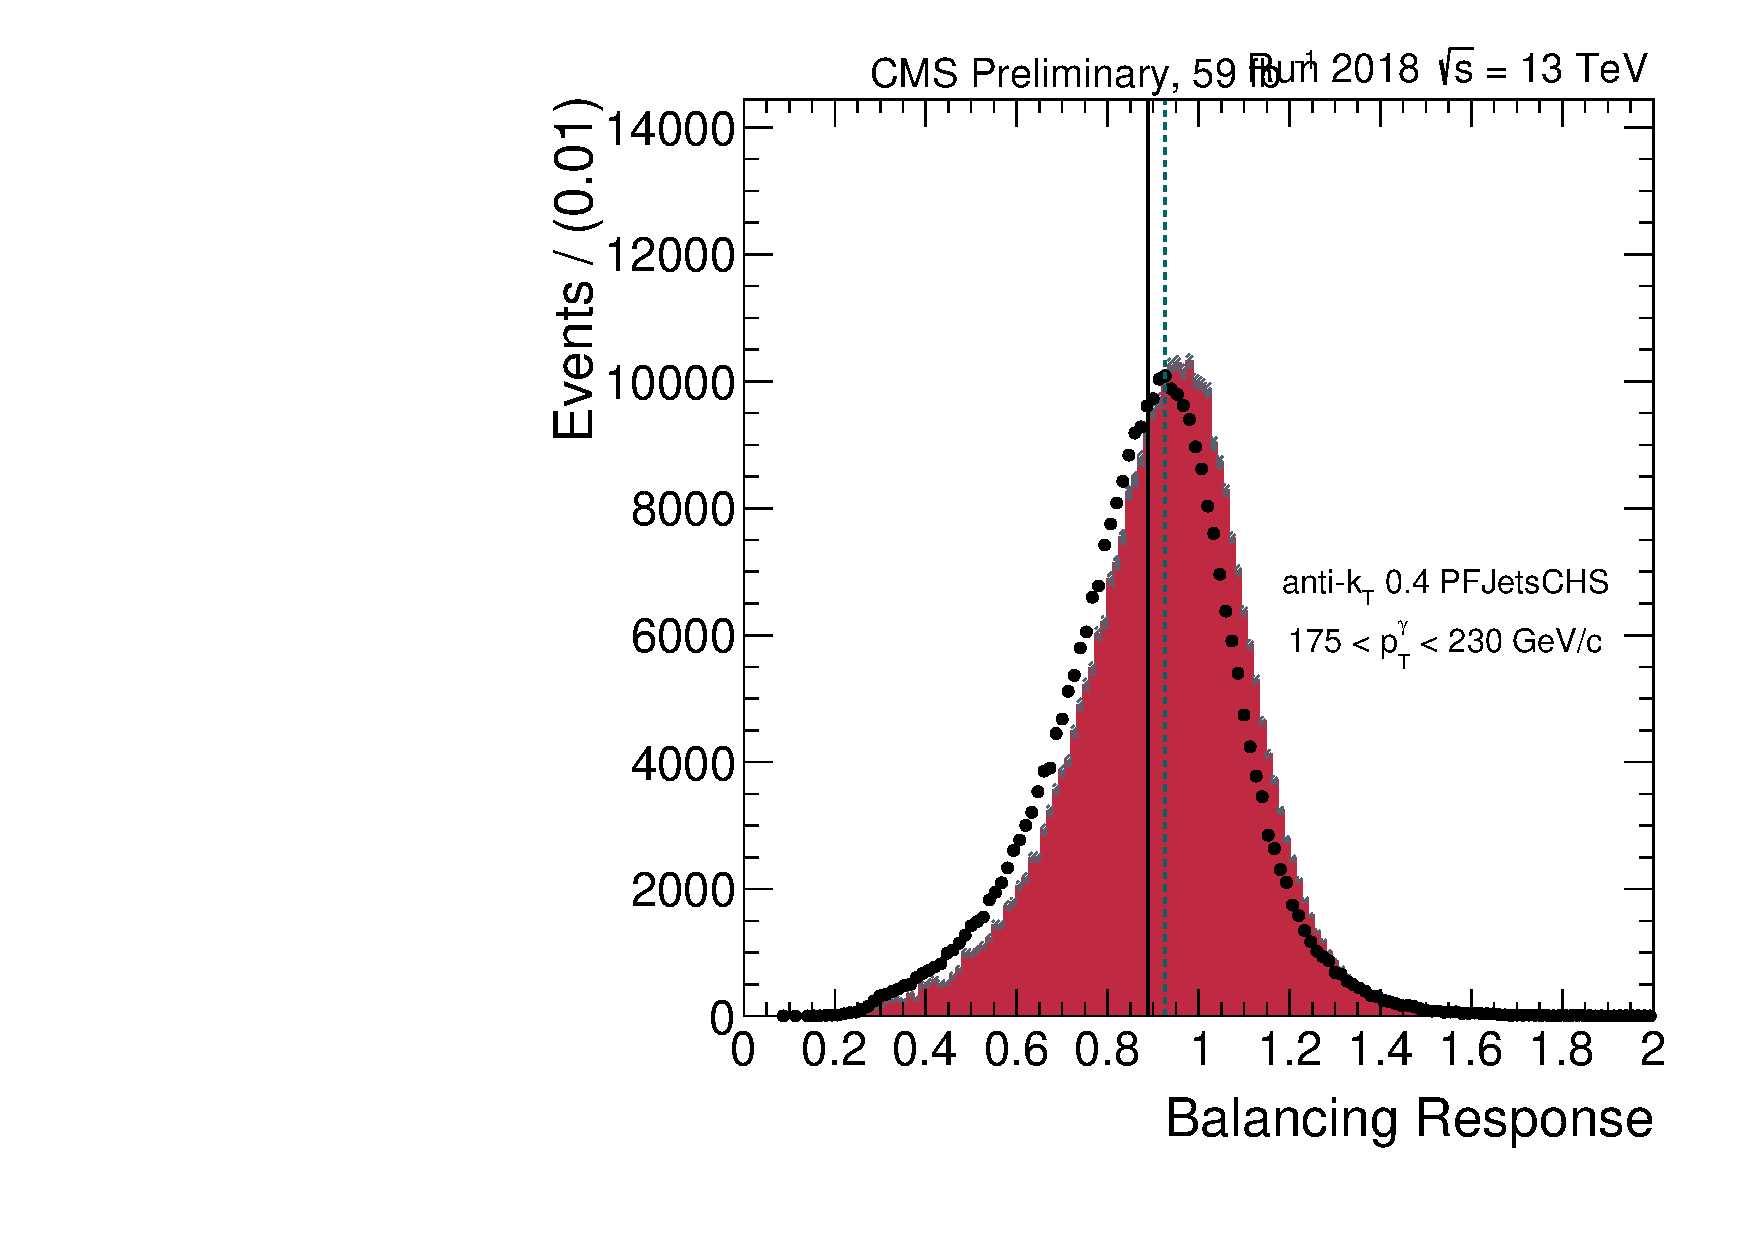
\includegraphics[width=.45\textwidth]{\PhDthesisdir/plots_and_images/my_plots/JERC/distributions/2018/with_header/resp_balancing_eta0013_ptPhot_175_230.tex}}
\hfill
\subcaptionbox{Réponse balancée pour $\pT^{\photon}\in[300, 400[$ \SI{}{\GeV}.\label{subfig-distrib_Gjets_18_resp_balancing_eta0013_ptPhot_300_400}}[.45\textwidth]
{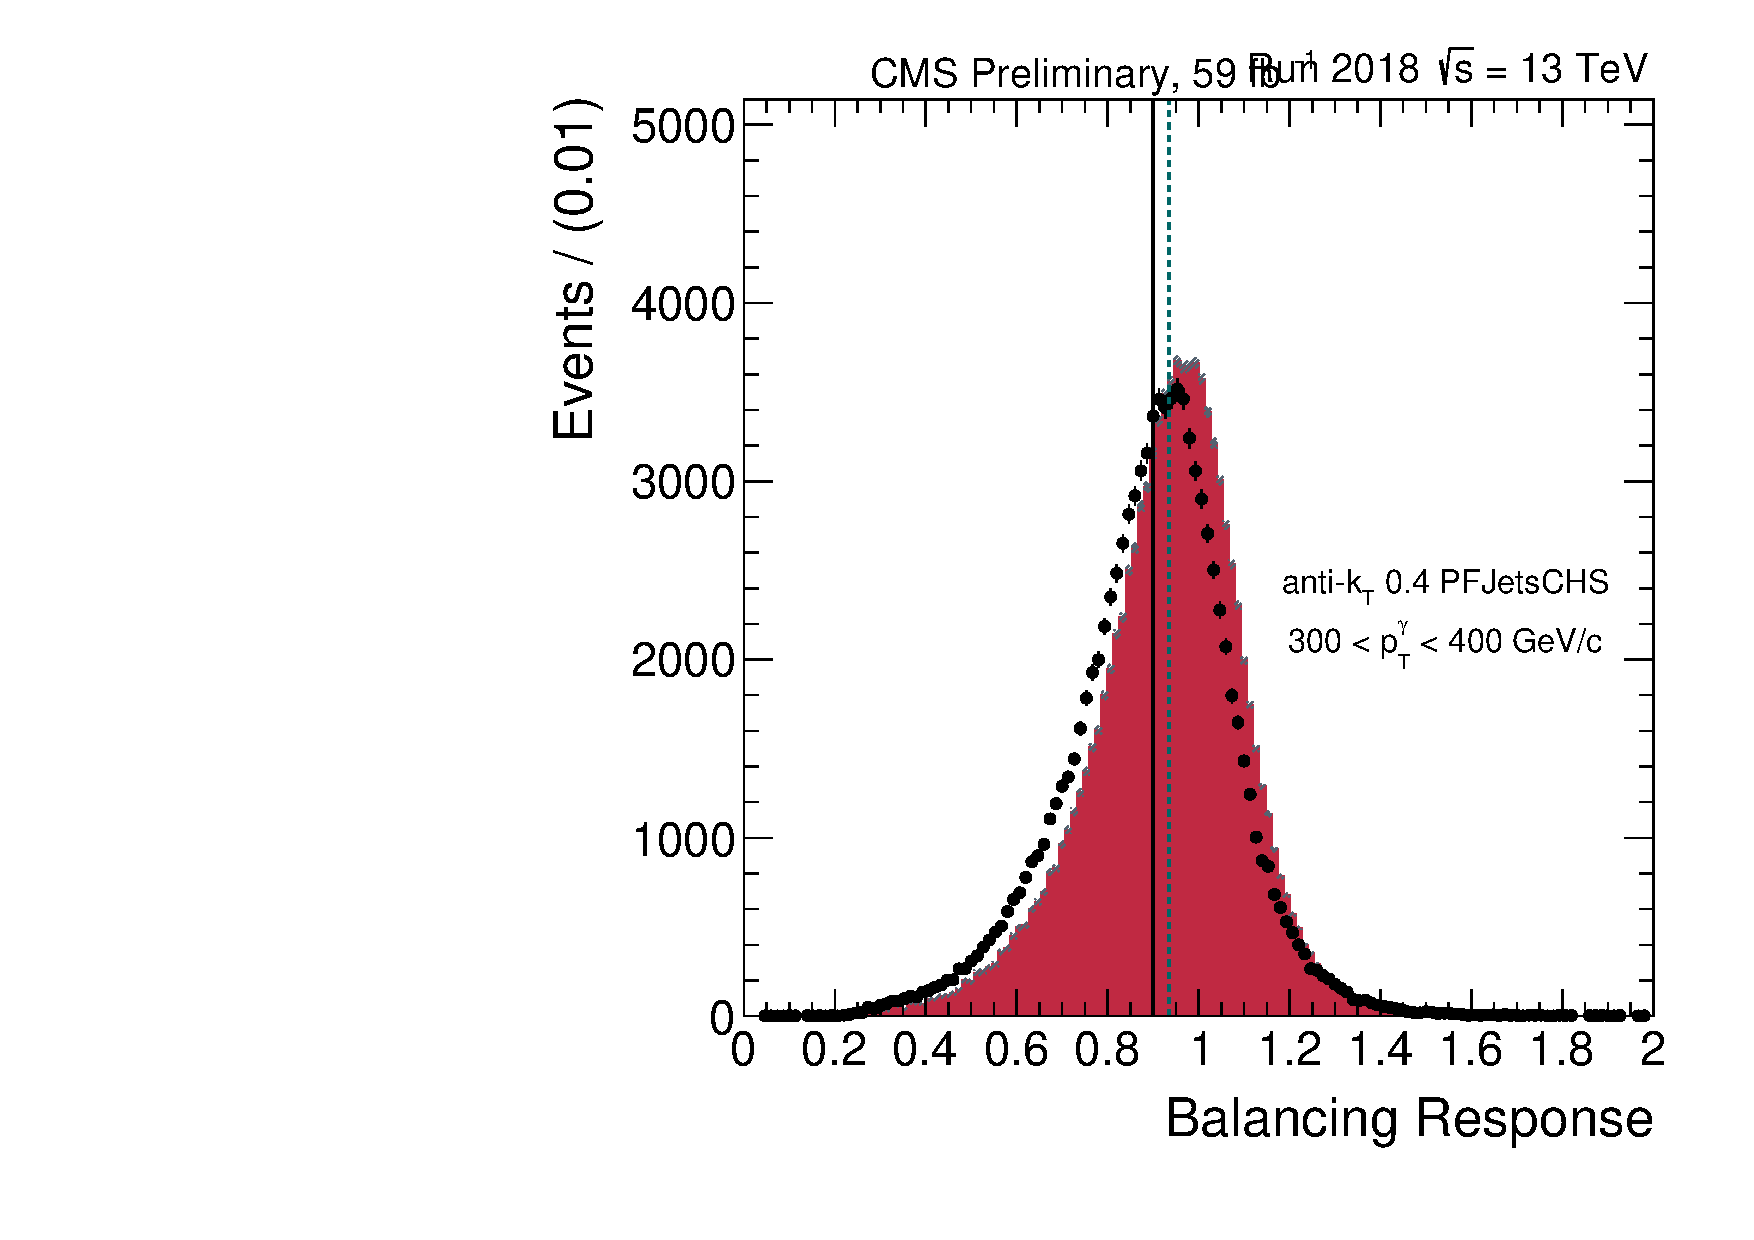
\includegraphics[width=.45\textwidth]{\PhDthesisdir/plots_and_images/my_plots/JERC/distributions/2018/with_header/resp_balancing_eta0013_ptPhot_300_400.tex}}

\vspace{.5\baselineskip}

\subcaptionbox{Réponse MPF pour $\pT^{\photon}\in[175, 230[$ \SI{}{\GeV}.\label{subfig-distrib_Gjets_18_resp_mpf_eta0013_ptPhot_175_230}}[.45\textwidth]
{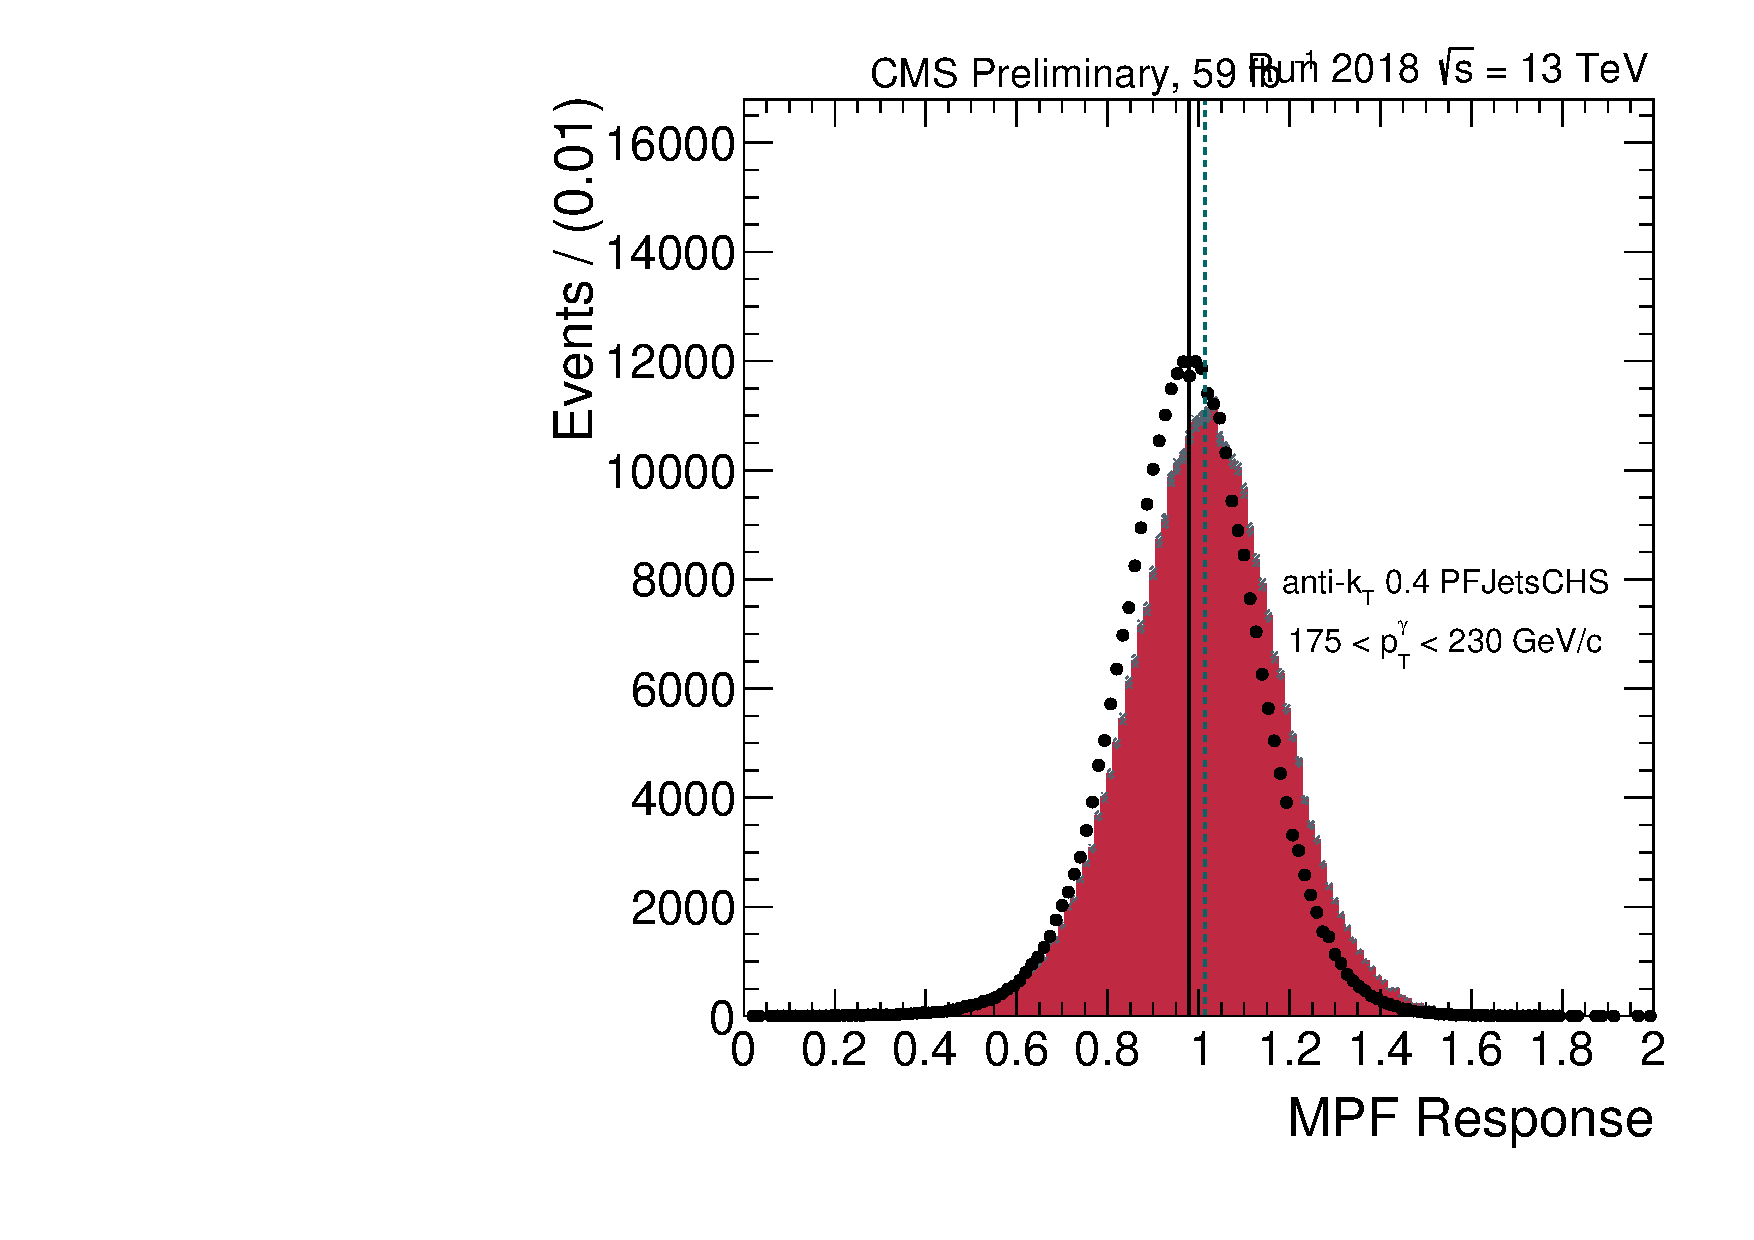
\includegraphics[width=.45\textwidth]{\PhDthesisdir/plots_and_images/my_plots/JERC/distributions/2018/with_header/resp_mpf_eta0013_ptPhot_175_230.tex}}
\hfill
\subcaptionbox{Réponse MPF pour $\pT^{\photon}\in[300, 400[$ \SI{}{\GeV}.\label{subfig-distrib_Gjets_18_resp_mpf_eta0013_ptPhot_300_400}}[.45\textwidth]
{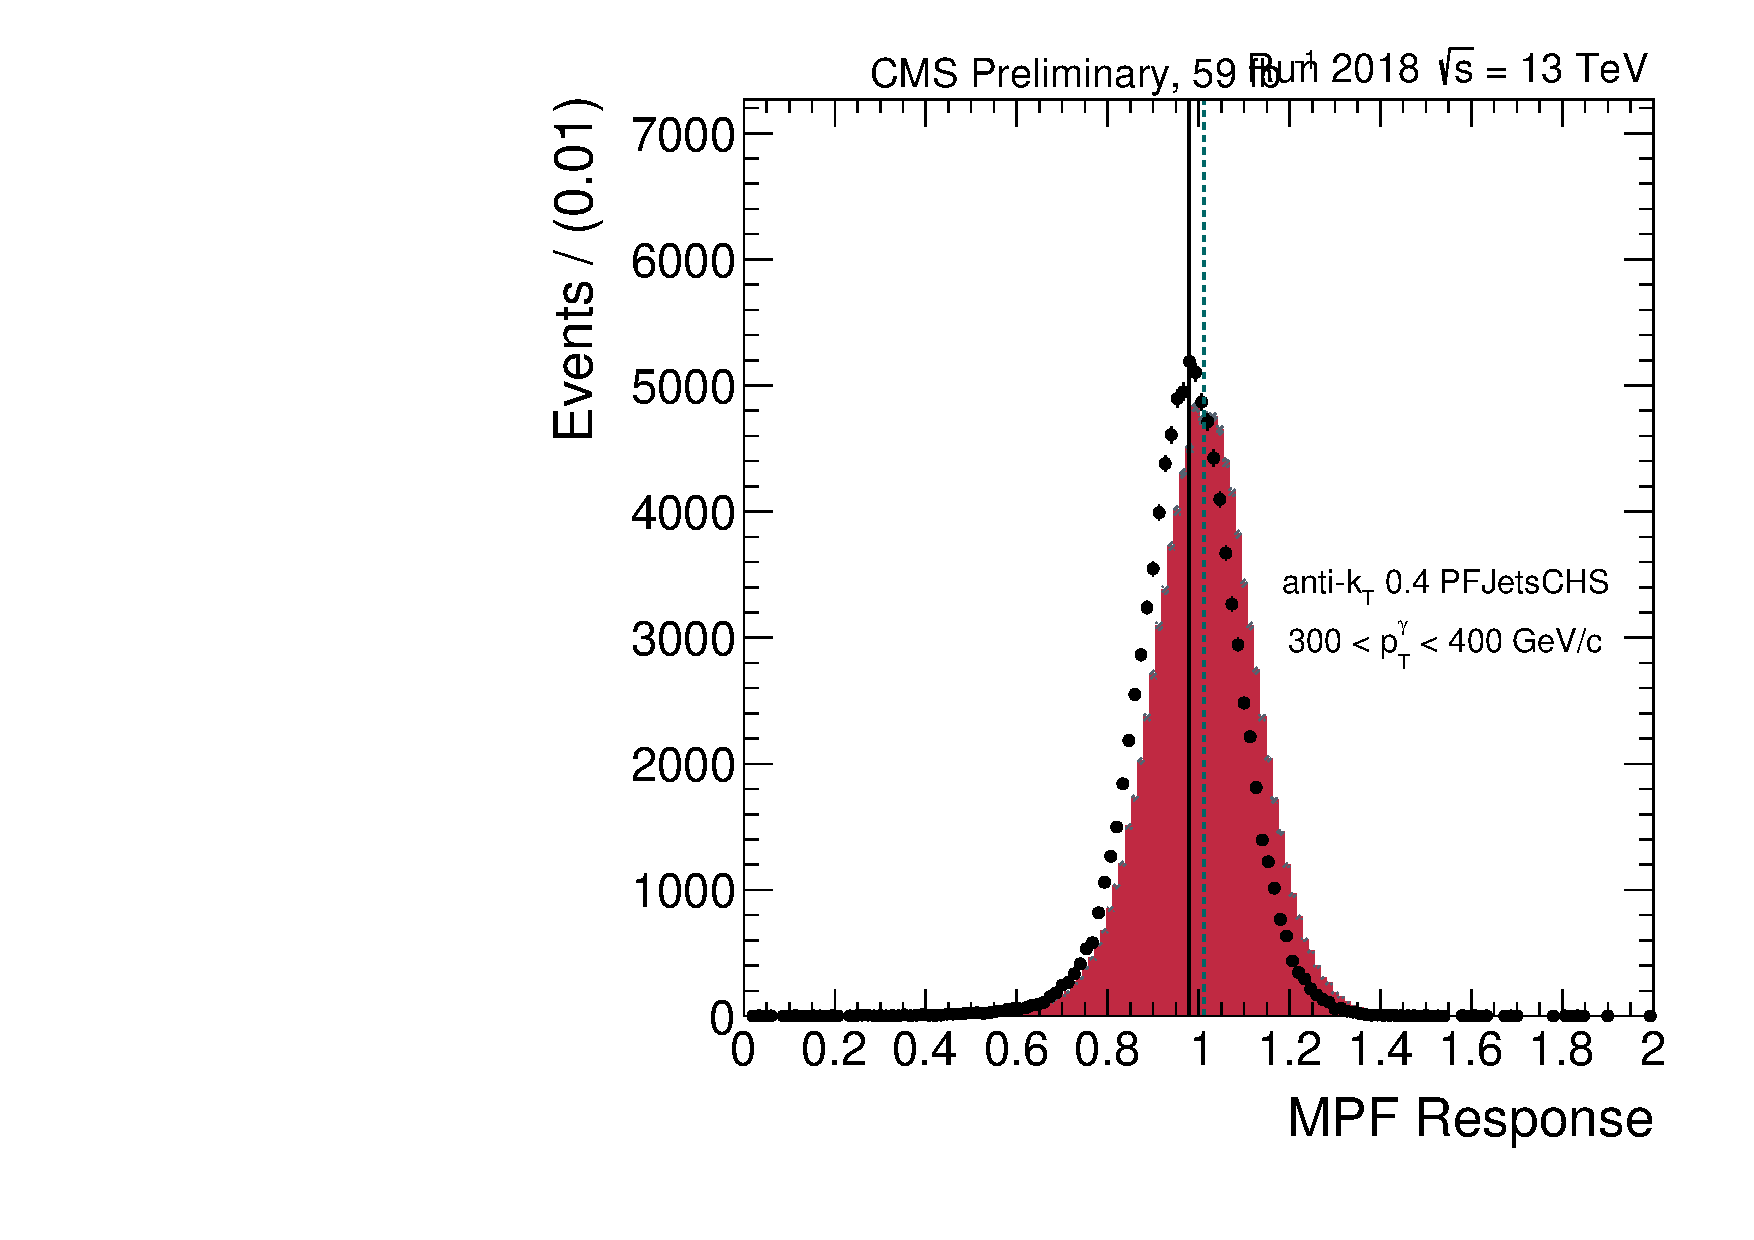
\includegraphics[width=.45\textwidth]{\PhDthesisdir/plots_and_images/my_plots/JERC/distributions/2018/with_header/resp_mpf_eta0013_ptPhot_300_400.tex}}

\caption[Réponses balancée et MPF en 2018.]{Réponses balancée et MPF dans les données (points noirs) et simulations (histogramme en rouge) pour $\alpha<\num{0.3}$, $\abs{\eta^\text{jet}}<\num{1.3}$ et deux intervalles de $\pT^{\photon}$ en 2018.}
\label{fig-distribs_Gjets_18_resp_bal_and_mpf}
\end{figure}
\paragraph{Extrapolation vers $\alpha=0$}
Une extrapolation vers $\alpha=0$ est réalisée afin de s'affranchir de l'activité additionnelle des jets décrite dans la section~\ref{chapter-JERC-section-pheno-GJets-subsec-effets_radiatifs}.
Les intervalles de $\alpha$ utilisés pour la JES sont présentés dans le tableau~\ref{tab-alpha_intervalles}.
L'utilisation des ces intervalles inclusifs permet une extrapolation linéaire en $\alpha$, ce qui est réalisé sur la figure~\ref{fig-chapter-JERC-section-JES-subsec-analyse-responsebal_and_MPF_eta0013_ptPhot_175_230_extrap}.
\begin{figure}[h]
\centering
\subcaptionbox{Réponse balancée.\label{subfig-chapter-JERC-section-JES-subsec-analyse-response_eta0013_ptPhot_175_230_extrap}}[.45\textwidth]
{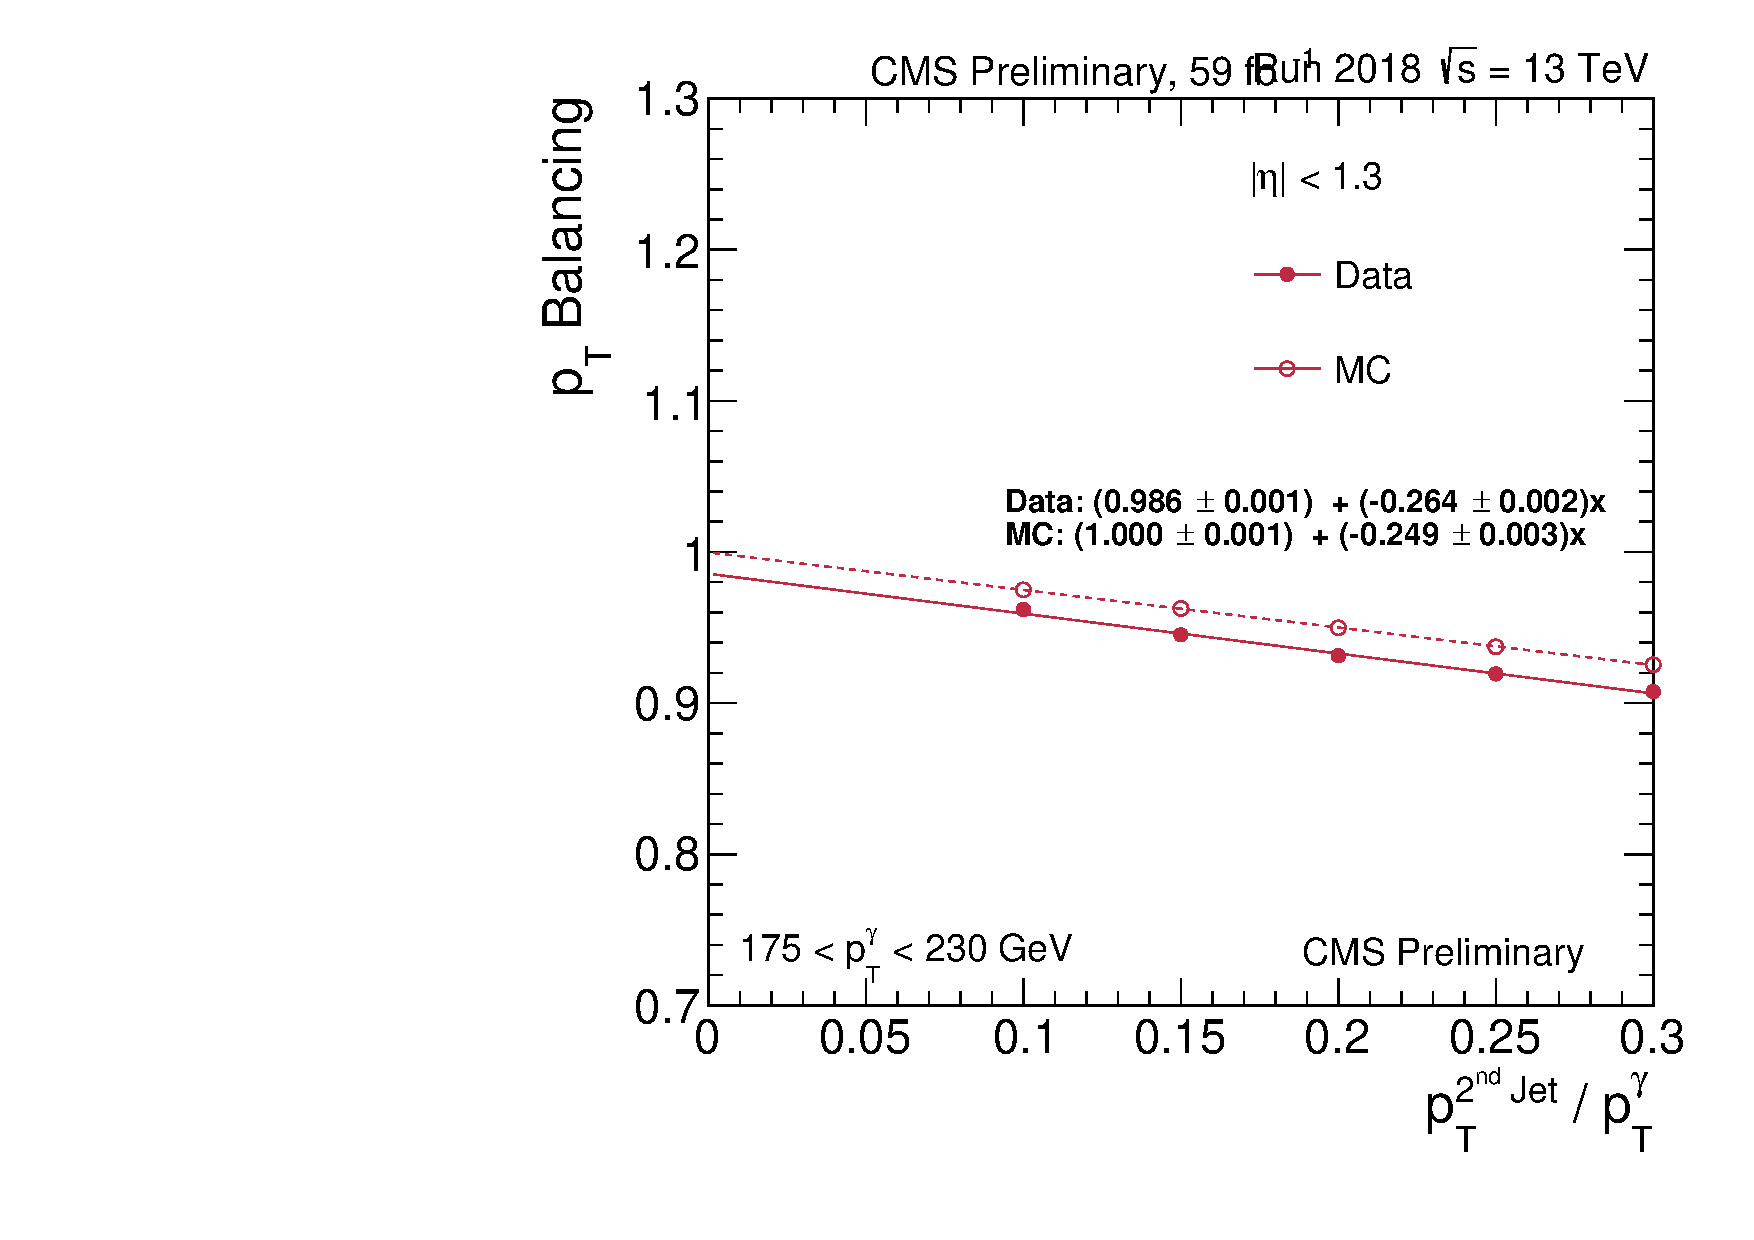
\includegraphics[width=.45\textwidth]{\PhDthesisdir/plots_and_images/my_plots/JERC/only_L2Res/Run2018ABCD/extrapolation/response_eta0013_ptPhot_175_230.tex}}
\hfill
\subcaptionbox{Réponse MPF.\label{subfig-chapter-JERC-section-JES-subsec-analyse-responseMPF_eta0013_ptPhot_175_230_extrap}}[.45\textwidth]
{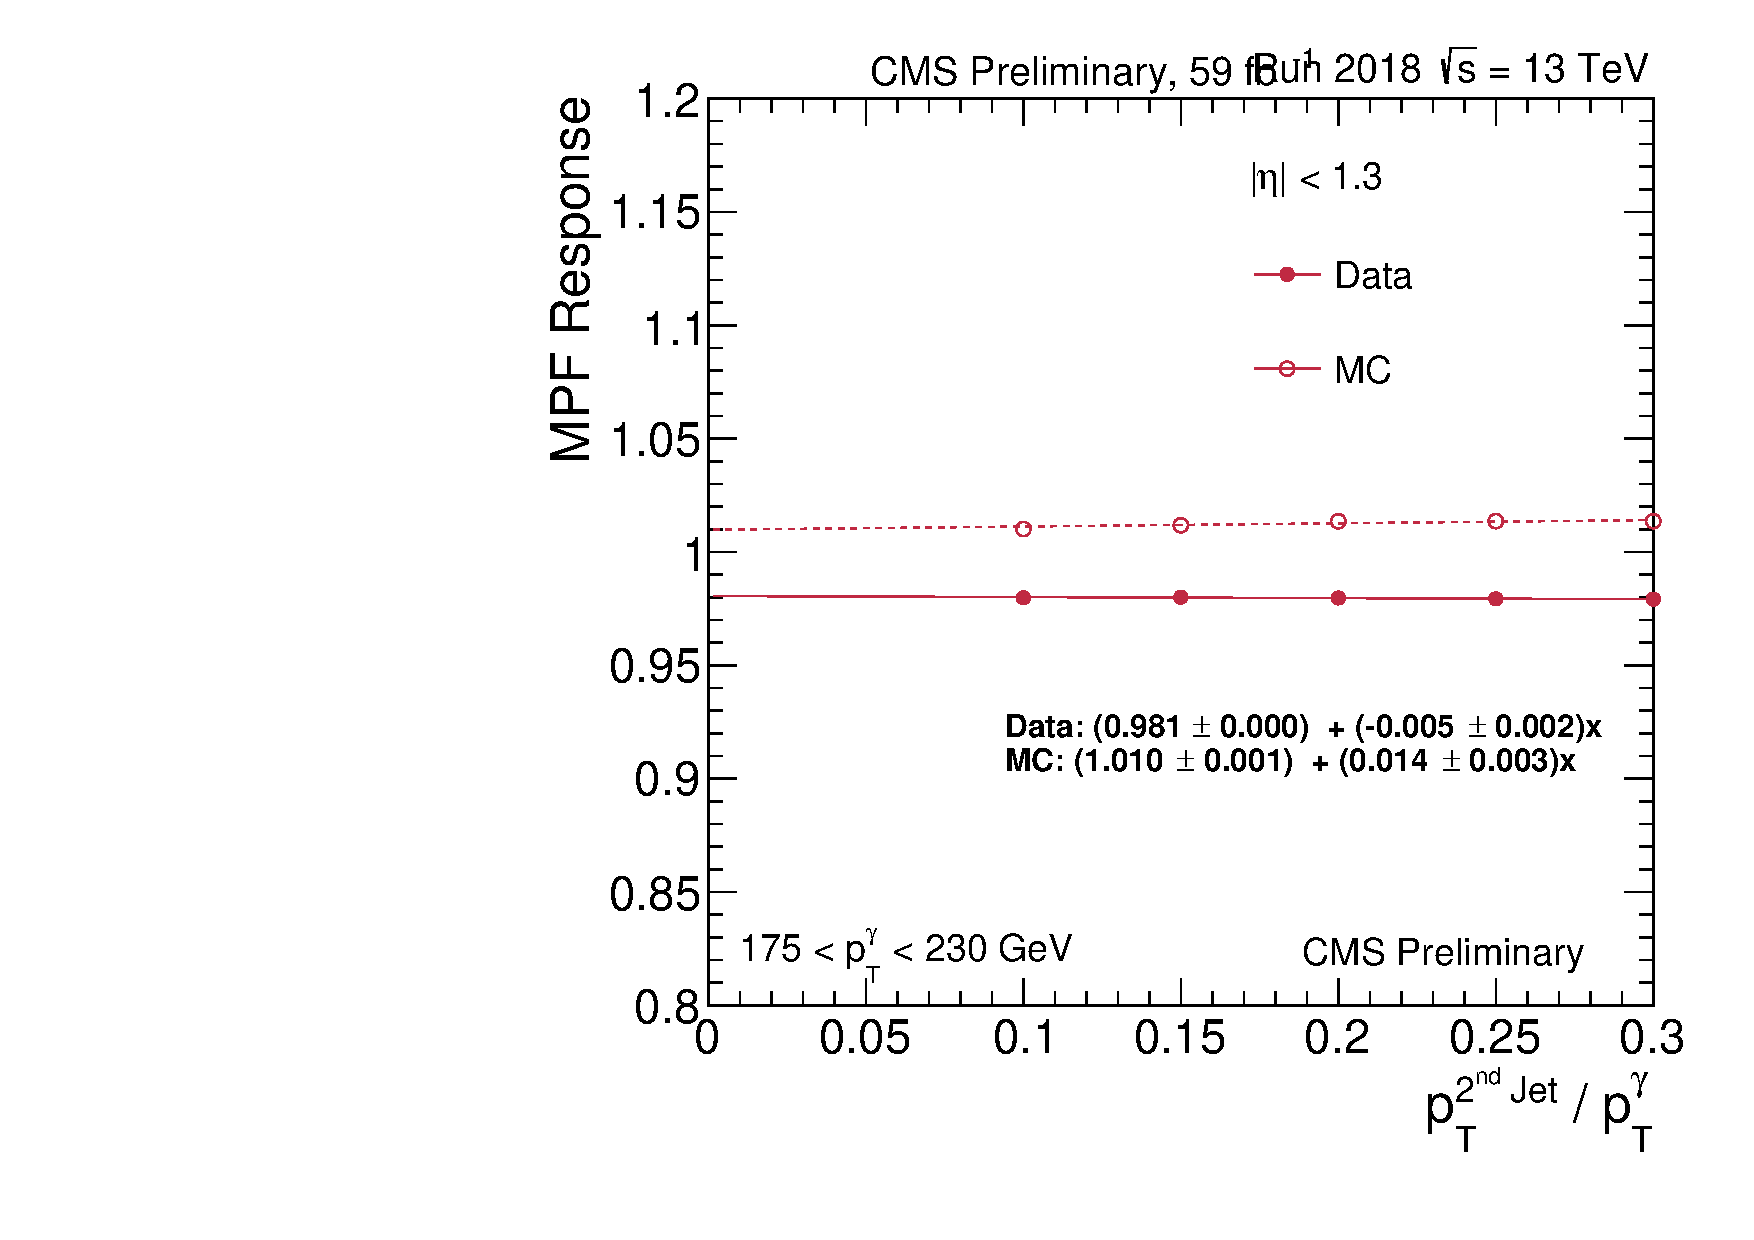
\includegraphics[width=.45\textwidth]{\PhDthesisdir/plots_and_images/my_plots/JERC/only_L2Res/Run2018ABCD/extrapolation/responseMPF_eta0013_ptPhot_175_230.tex}}
\caption[Extrapolation vers $\alpha=0$ de la réponse des jets.]{Extrapolation vers $\alpha=0$ de la réponse des jets pour $\abs{\eta}<\num{1.3}$ et $\num{175}<\pT^{\photon}<\SI{230}{\GeV}$ en 2018.}
\label{fig-chapter-JERC-section-JES-subsec-analyse-responsebal_and_MPF_eta0013_ptPhot_175_230_extrap}
\end{figure}
\subsection{Résultats}\label{chapter-JERC-section-JES-subsec-results}
La correction à appliquer aux données, définie par la formule~\eqref{eq-chapter-JERC-section-CMS-subsec-residuals-Cres_def} d'après la démarche exposée dans la section~\ref{chapter-JERC-section-CMS-subsec-residuals}, s'obtient en calculant la valeur moyenne des réponses \Rbal\ ou \RMPF\ pour les données et les simulations dans chacun des intervalles
de $\pT^{\photon}$ défini dans le tableau~\ref{tab-pT_photon_intervalles} et
de $\eta^\text{jet}$ défini dans le tableau~\ref{tab-eta_jet_intervalles_large}.
Elle permet de ramener la réponse moyenne des jets dans les données à celle constatée dans les simulations.
\par Les résultats ainsi obtenus à l'aide des méthodes de la balance et MPF, avant et après extrapolation vers $\alpha=0$, sont présentés dans les sections~\ref{chapter-JERC-section-JES-subsec-results-subsubsec-before_extrap} et~\ref{chapter-JERC-section-JES-subsec-results-subsubsec-after_extrap}.
Les distributions moyennes des réponses en fonction de $\pT^{\photon}$ dans les données et les simulations, ainsi que leurs rapports, y sont représentés.
Un ajustement constant est réalisé dans chaque intervalle de $\eta^\text{jet}$ afin d'obtenir un ordre de grandeur de la correction à appliquer dans cet intervalle.
La dépendance en $\pT$ de la correction est déterminée grâce à un ajustement global réalisé avec les résultats d'autres analyses, présenté dans la section~\ref{chapter-JERC-section-JES-subsec-results-subsubsec-global_fit}.
Enfin, une vérification de la bonne mise en œuvre de la correction ainsi déterminée est présentée dans la section~\ref{chapter-JERC-section-JES-subsec-results-subsubsec-L2L3Res_cross_check}.
\subsubsection{Résultats avant extrapolation}\label{chapter-JERC-section-JES-subsec-results-subsubsec-before_extrap}
\par Les distributions des réponses balancées avant extrapolation se trouvent figure~\ref{fig-responses_balancing_alpha_0_3_2018ABCD}, page~\pageref{fig-responses_balancing_alpha_0_3_2018ABCD}.
Les corrections à appliquer sont de l'ordre
de \SI{4}{\%} pour $\abs{\eta^\text{jet}} < \num{1.3}$,
de \SI{6}{\%} pour $\num{1.3} \leq \abs{\eta^\text{jet}} < \num{2.5}$ et
de \SI{3}{\%} pour $\abs{\eta^\text{jet}} > \num{2.5}$.
\par Les distributions des réponses MPF avant extrapolation se trouvent figure~\ref{fig-responses_MPF_alpha_0_3_2018ABCD}, page~\pageref{fig-responses_MPF_alpha_0_3_2018ABCD}.
Les corrections à appliquer sont de l'ordre
de \SI{3}{\%} pour $\abs{\eta^\text{jet}} < \num{1.3}$,
de \SI{5}{\%} pour $\num{1.3} \leq \abs{\eta^\text{jet}} < \num{2.5}$, soit environ \SI{1}{\%} de moins qu'avec la méthode balancée, et
de \SI{3}{\%} pour $\abs{\eta^\text{jet}} > \num{2.5}$,
\par Il est à noter que ces résultats sont obtenus avant extrapolation vers $\alpha=0$. Or, cette extrapolation a un effet beaucoup plus important sur la réponse balancée que sur la réponse MPF, comme le montre la figure~\ref{fig-chapter-JERC-section-JES-subsec-analyse-responsebal_and_MPF_eta0013_ptPhot_175_230_extrap}.
\subsubsection{Résultats après extrapolation}\label{chapter-JERC-section-JES-subsec-results-subsubsec-after_extrap}
L'extrapolation des réponses vers $\alpha=0$ est réalisée comme expliqué dans la section~\ref{chapter-JERC-section-JES-subsec-analyse}.
\par Les distributions des réponses balancées après extrapolation se trouvent figure~\ref{fig-responses_balancing_extrapolated_2018ABCD}, page~\pageref{fig-responses_balancing_extrapolated_2018ABCD}.
Les corrections à appliquer sont de l'ordre
de \SI{3}{\%} pour $\abs{\eta^\text{jet}} < \num{1.3}$,
de \SI{5}{\%} pour $\num{1.3} \leq \abs{\eta^\text{jet}} < \num{2.5}$, soit environ \SI{1}{\%} de moins qu'avant extrapolation, et
de \SI{3}{\%} pour $\abs{\eta^\text{jet}} > \num{2.5}$.
\par Les distributions des réponses MPF après extrapolation se trouvent figure~\ref{fig-responses_MPF_extrapolated_2018ABCD}, page~\pageref{fig-responses_MPF_extrapolated_2018ABCD}.
Les corrections à appliquer sont de l'ordre
de \SI{3}{\%} pour $\abs{\eta^\text{jet}} < \num{1.3}$,
de \SI{5}{\%} pour $\num{1.3} \leq \abs{\eta^\text{jet}} < \num{2.5}$ et
de \SI{3}{\%} pour $\abs{\eta^\text{jet}} > \num{2.5}$,
soit du même ordre qu'avant extrapolation.
L'extrapolation a donc bien un effet très faible sur \RMPF.
\par Les valeurs des rapports données sur simulations des réponses balancée et MPF obtenus sont résumés dans le tableau~\ref{tab-responses_recap_table_2018ABCD}.
L'extrapolation vers $\alpha=0$ permet de rétablir l'accord entre les rapport des réponses balancée et MPF.
Cet accord permet de valider l'utilisation de ces méthodes afin d'estimer la JES.

\begin{table}[h]
\centering
\begin{tabular}{lcccc}
\toprule
\multirow{2}{*}{$\abs{\eta^\text{jet}}\in$} & \multicolumn{2}{c}{Réponse balancée} & \multicolumn{2}{c}{Réponse MPF} \\
\cmidrule(lr){2-3}\cmidrule(lr){4-5}
 & $\alpha<\num{0.3}$ & $\alpha\to0$ & $\alpha<\num{0.3}$ & $\alpha\to0$\\
\midrule
$[\num{0}\isp \num{1.3}[$ & $\num{0.9581}\pm\num{0.0003}$ & $\num{0.9669}\pm\num{0.0004}$ & $\num{0.9667}\pm\num{0.0002}$ & $\num{0.9687}\pm\num{0.0003}$ \\
$[\num{1.3}\isp \num{2.0}[$ & $\num{0.9426}\pm\num{0.0006}$ & $\num{0.9538}\pm\num{0.0009}$ & $\num{0.9521}\pm\num{0.0004}$ & $\num{0.9565}\pm\num{0.0008}$ \\
$[\num{2.0}\isp \num{2.5}[$ & $\num{0.9425}\pm\num{0.0010}$ & $\num{0.9502}\pm\num{0.0015}$ & $\num{0.9508}\pm\num{0.0007}$ & $\num{0.9516}\pm\num{0.0014}$ \\
$[\num{2.5}\isp \num{3.0}[$ & $\num{0.9744}\pm\num{0.0026}$ & $\num{0.9661}\pm\num{0.0037}$ & $\num{0.9689}\pm\num{0.0018}$ & $\num{0.9707}\pm\num{0.0034}$ \\
\bottomrule
\end{tabular}
\caption[Rapports des réponses balancée et MPF obtenus en 2018.]{Rapports données réelles sur simulées des réponses balancée et MPF obtenus en 2018.}
\label{tab-responses_recap_table_2018ABCD}
\end{table}

\begin{figure}[p]
\centering
\subcaptionbox{$\abs{\eta^\text{jet}} < \num{1.3}$.\label{subfig-response_eta0013_balancing_alpha_0_3_2018ABCD}}[.45\textwidth]
{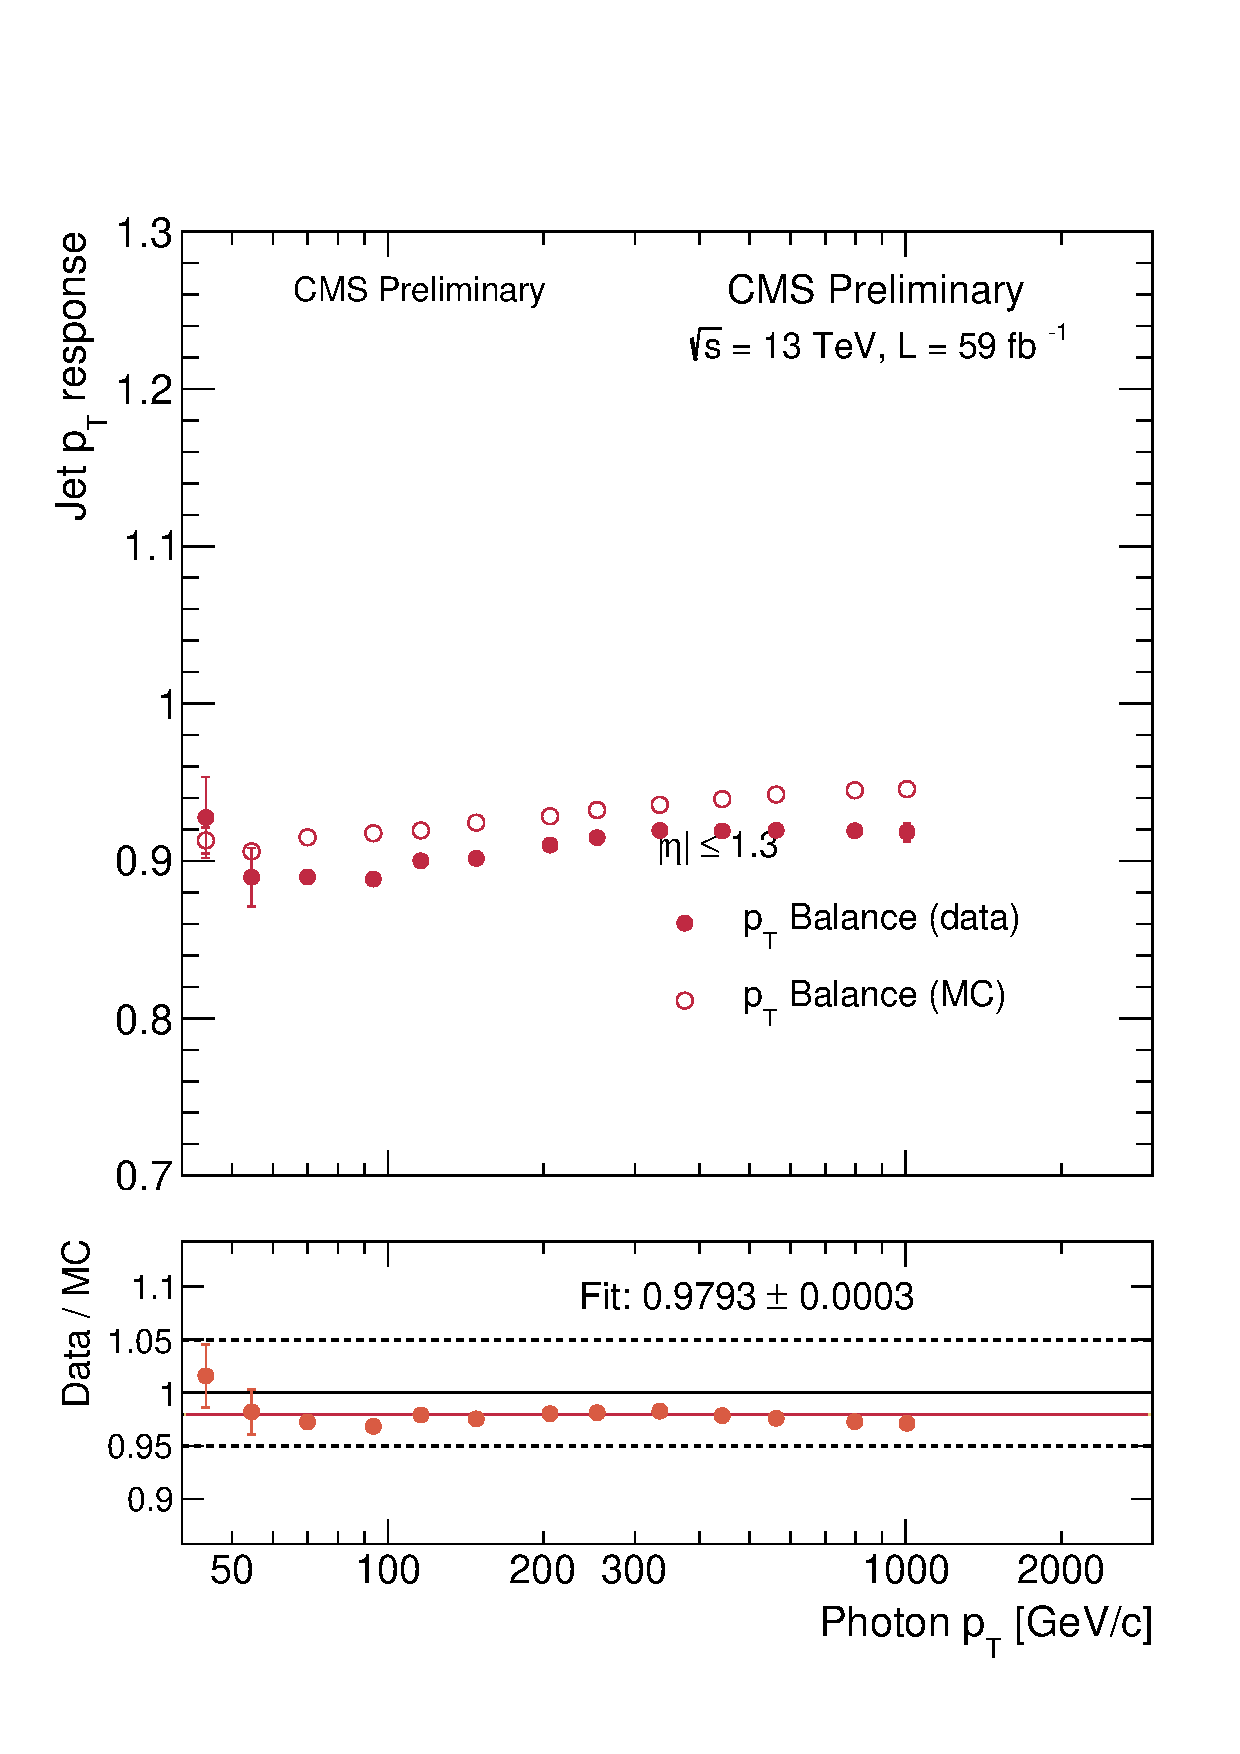
\includegraphics[width=.45\textwidth]{\PhDthesisdir/plots_and_images/my_plots/JERC/only_L2Res/Run2018ABCD/alpha_0_3/response_eta0013_balancing.pdf}}
\hfill
\subcaptionbox{$\num{1.3} \leq \abs{\eta^\text{jet}} < \num{2.0}$.\label{subfig-response_eta1319_balancing_alpha_0_3_2018ABCD}}[.45\textwidth]
{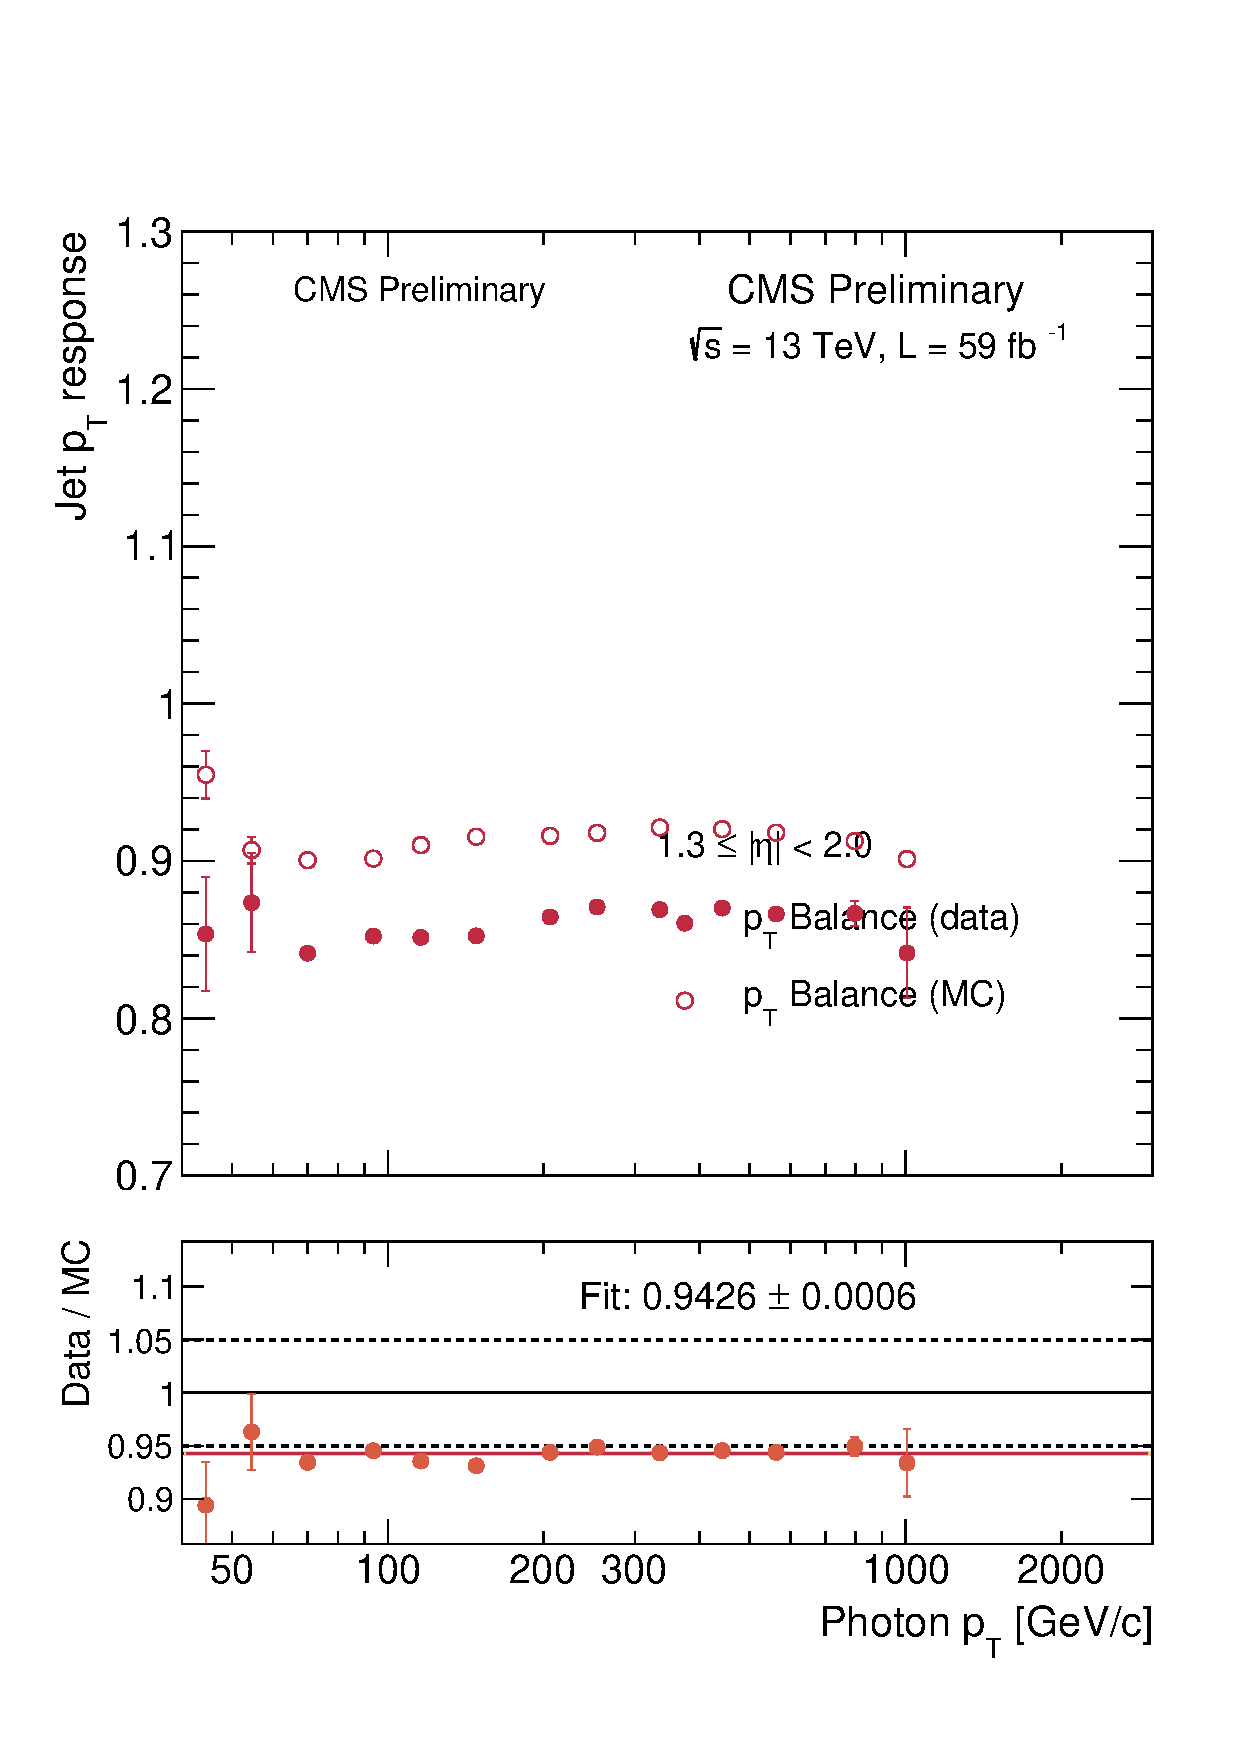
\includegraphics[width=.45\textwidth]{\PhDthesisdir/plots_and_images/my_plots/JERC/only_L2Res/Run2018ABCD/alpha_0_3/response_eta1319_balancing.pdf}}

\vfill

\subcaptionbox{$\num{2.0} \leq \abs{\eta^\text{jet}} < \num{2.5}$.\label{subfig-response_eta1925_balancing_alpha_0_3_2018ABCD}}[.45\textwidth]
{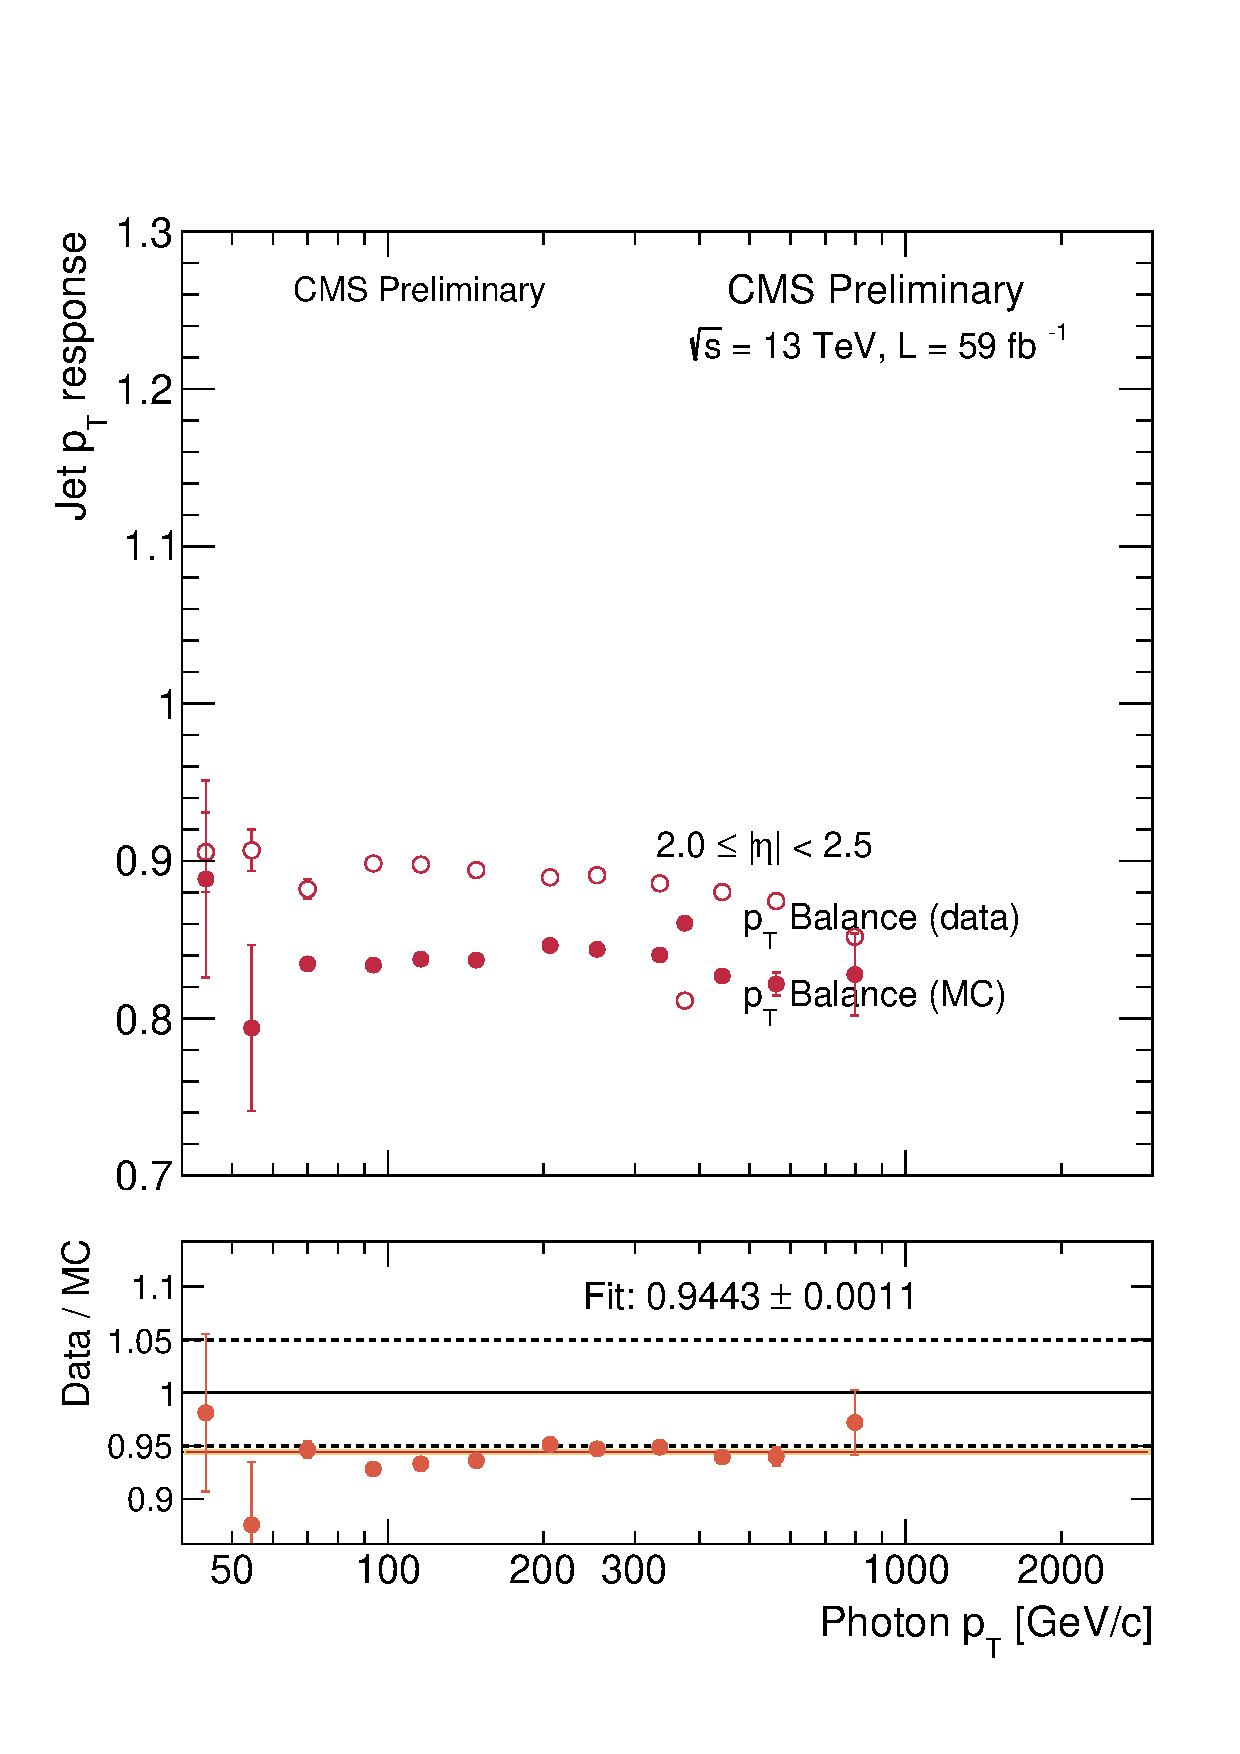
\includegraphics[width=.45\textwidth]{\PhDthesisdir/plots_and_images/my_plots/JERC/only_L2Res/Run2018ABCD/alpha_0_3/response_eta1925_balancing.pdf}}
\hfill
\subcaptionbox{$\num{2.5} \leq \abs{\eta^\text{jet}} < \num{3.0}$.\label{subfig-response_eta2530_balancing_alpha_0_3_2018ABCD}}[.45\textwidth]
{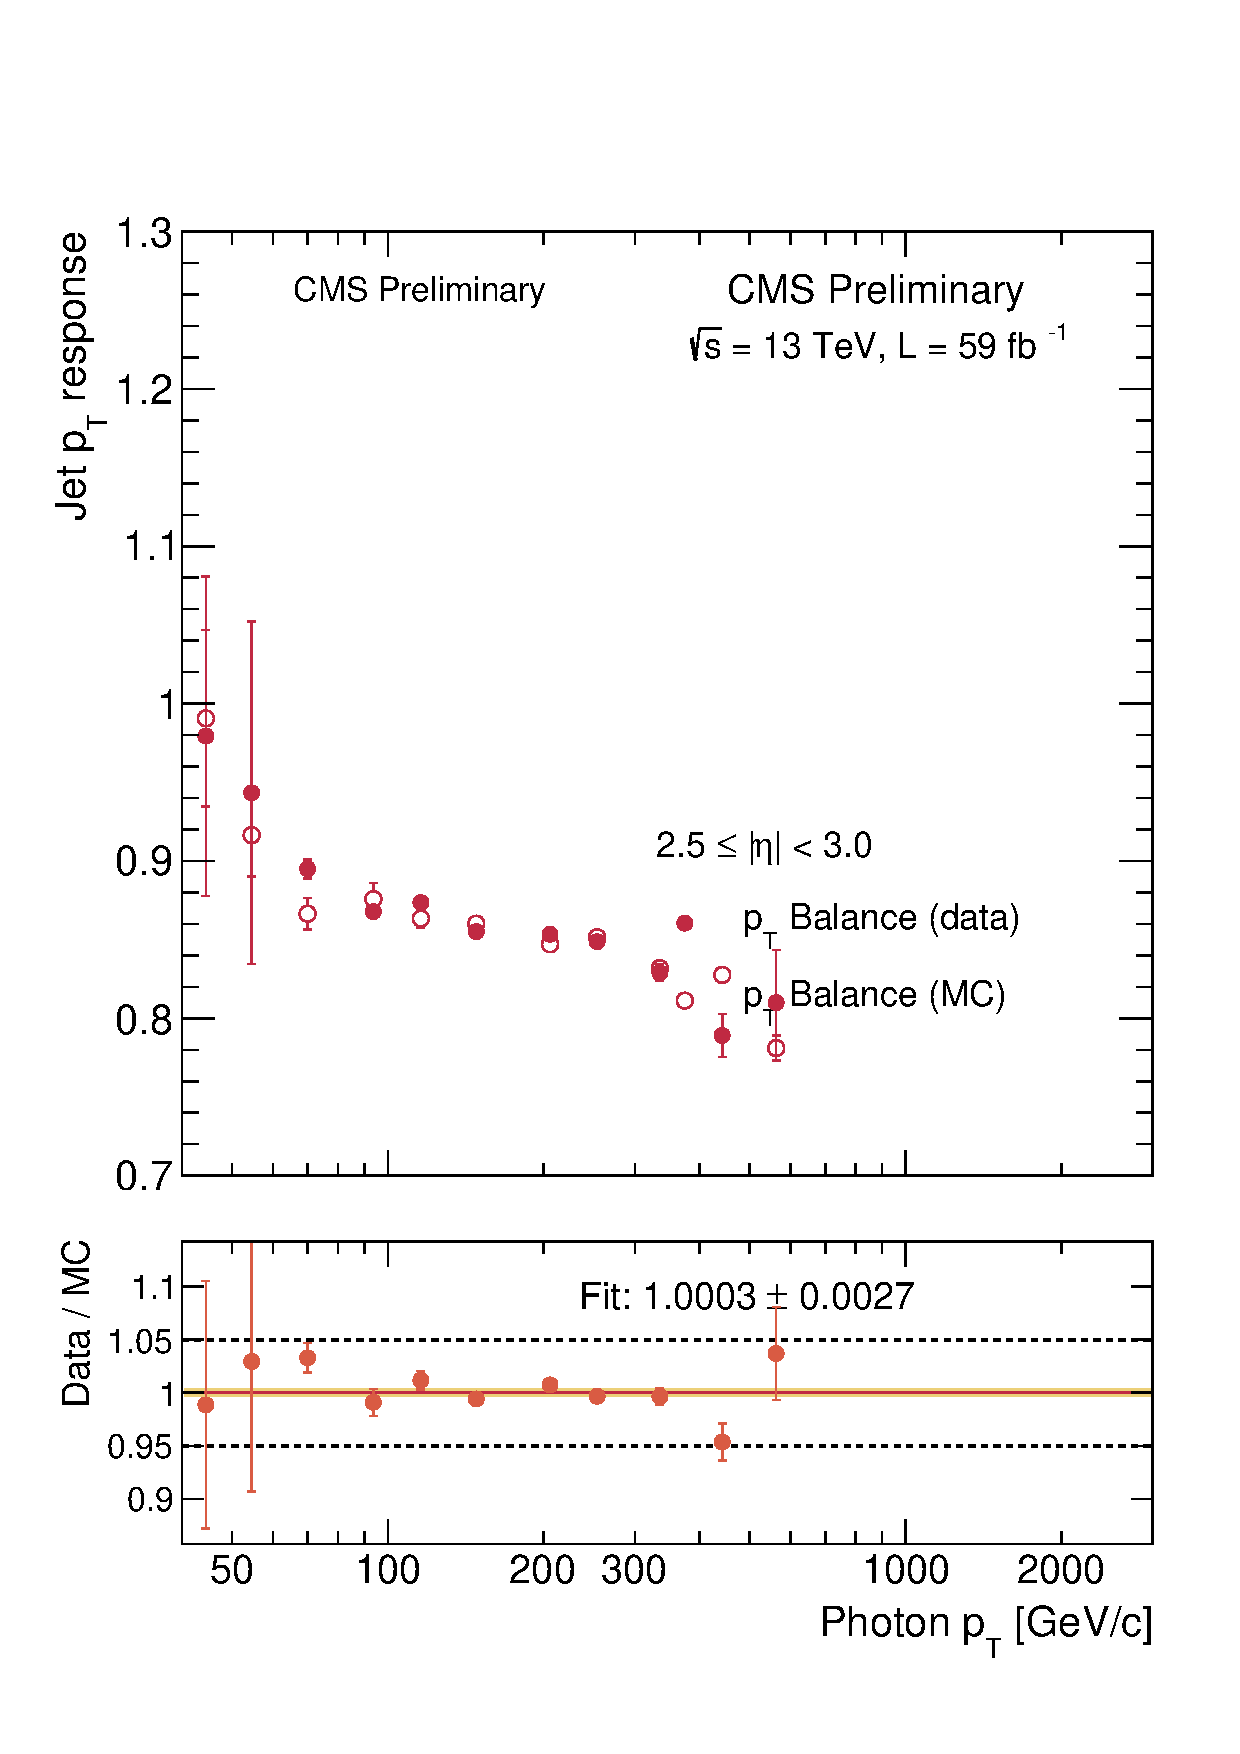
\includegraphics[width=.45\textwidth]{\PhDthesisdir/plots_and_images/my_plots/JERC/only_L2Res/Run2018ABCD/alpha_0_3/response_eta2530_balancing.pdf}}

\caption[Réponses balancées en 2018 avant extrapolation.]{Distributions des réponses balancées moyennes en fonction de $\pT^{\text{\photon}}$ pour différents intervalles de $\eta^\text{jet}$ en 2018 avant extrapolation. Le rapport données sur simulations est présenté dans chaque cas ainsi qu'un ajustement à une constante donnant l'ordre de grandeur de la correction résiduelle à appliquer.}
\label{fig-responses_balancing_alpha_0_3_2018ABCD}
\end{figure}
\begin{figure}[p]
\centering
\subcaptionbox{$\abs{\eta^\text{jet}} < \num{1.3}$.\label{subfig-response_eta0013_MPF_alpha_0_3_2018ABCD}}[.45\textwidth]
{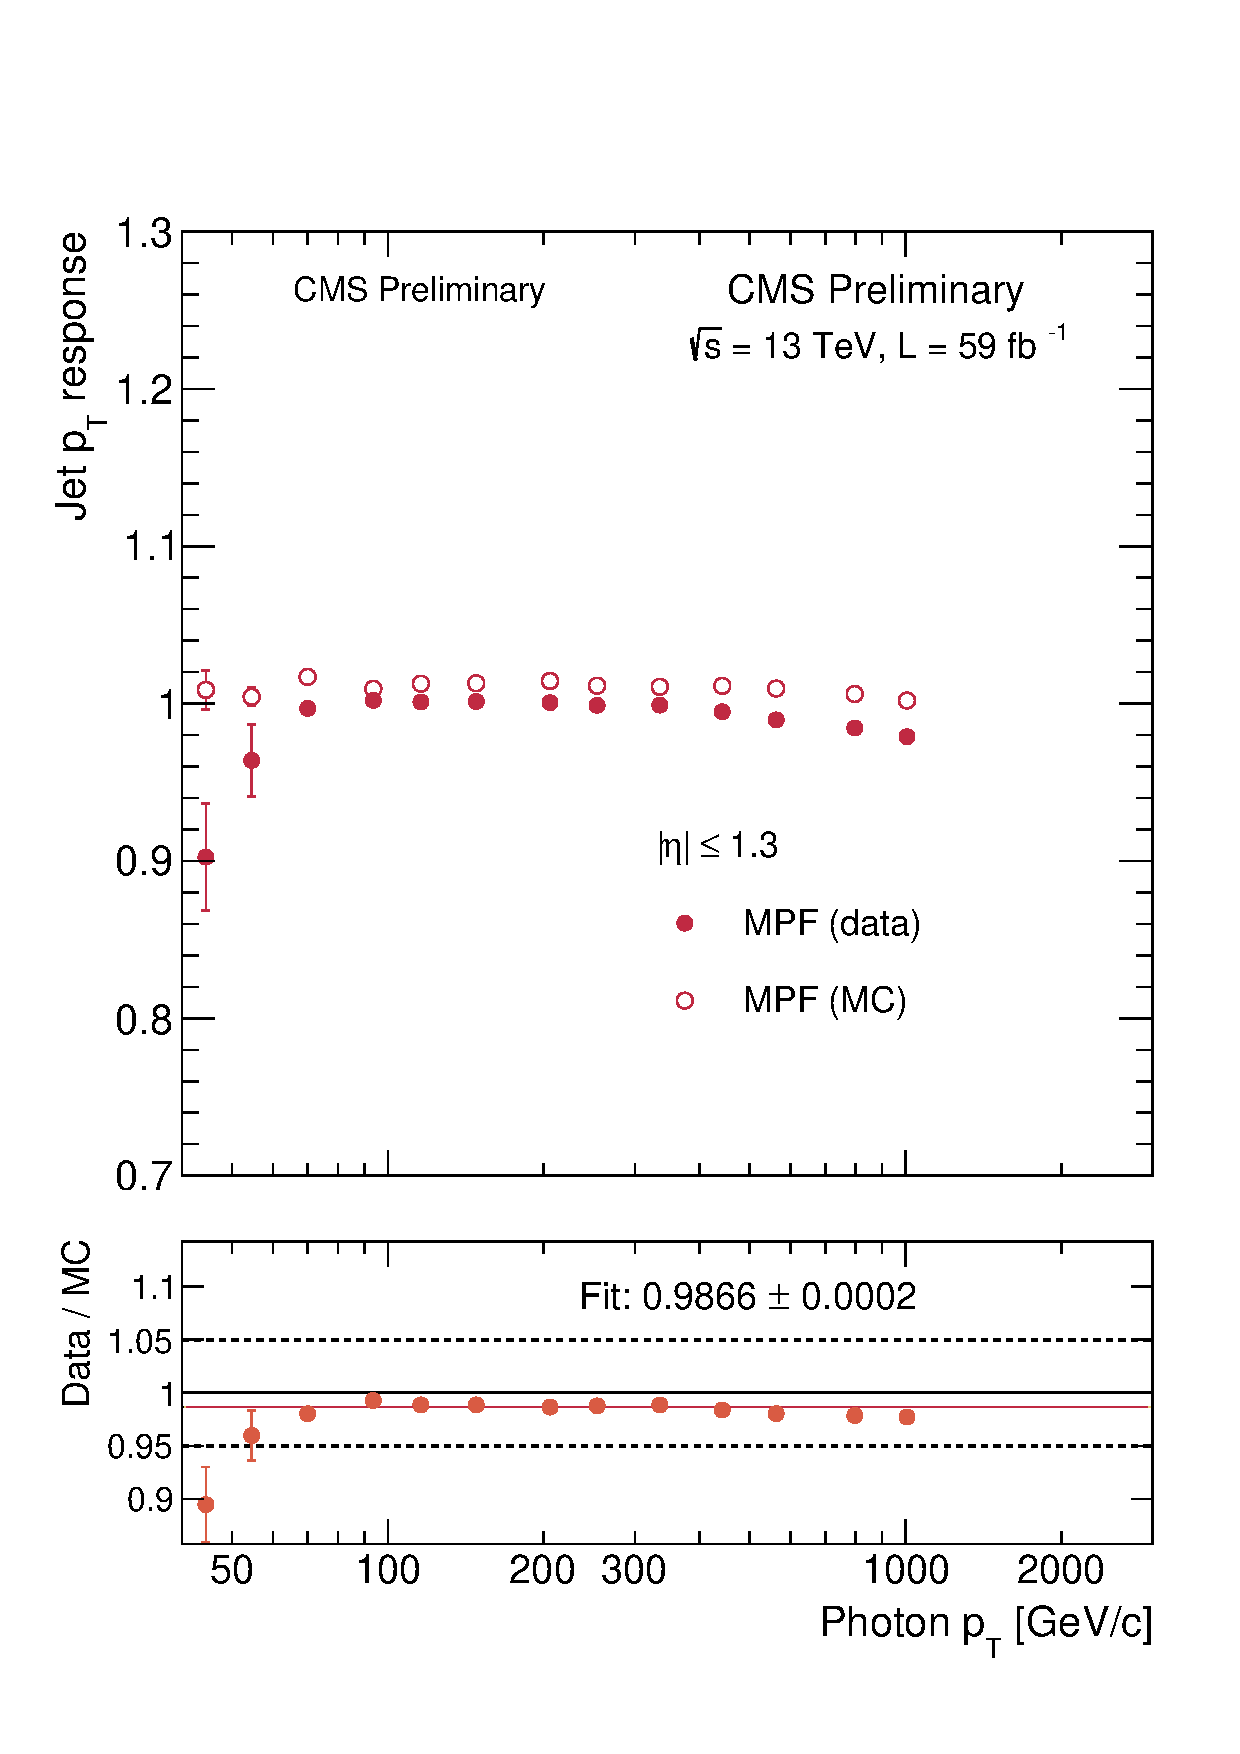
\includegraphics[width=.45\textwidth]{\PhDthesisdir/contents/chapter-JERC/plots/my_plots/only_L2Res/Run2018ABCD/alpha_0_3/response_eta0013_mpf.pdf}}
\hfill
\subcaptionbox{$\num{1.3} \leq \abs{\eta^\text{jet}} < \num{2.0}$.\label{subfig-response_eta1319_MPF_alpha_0_3_2018ABCD}}[.45\textwidth]
{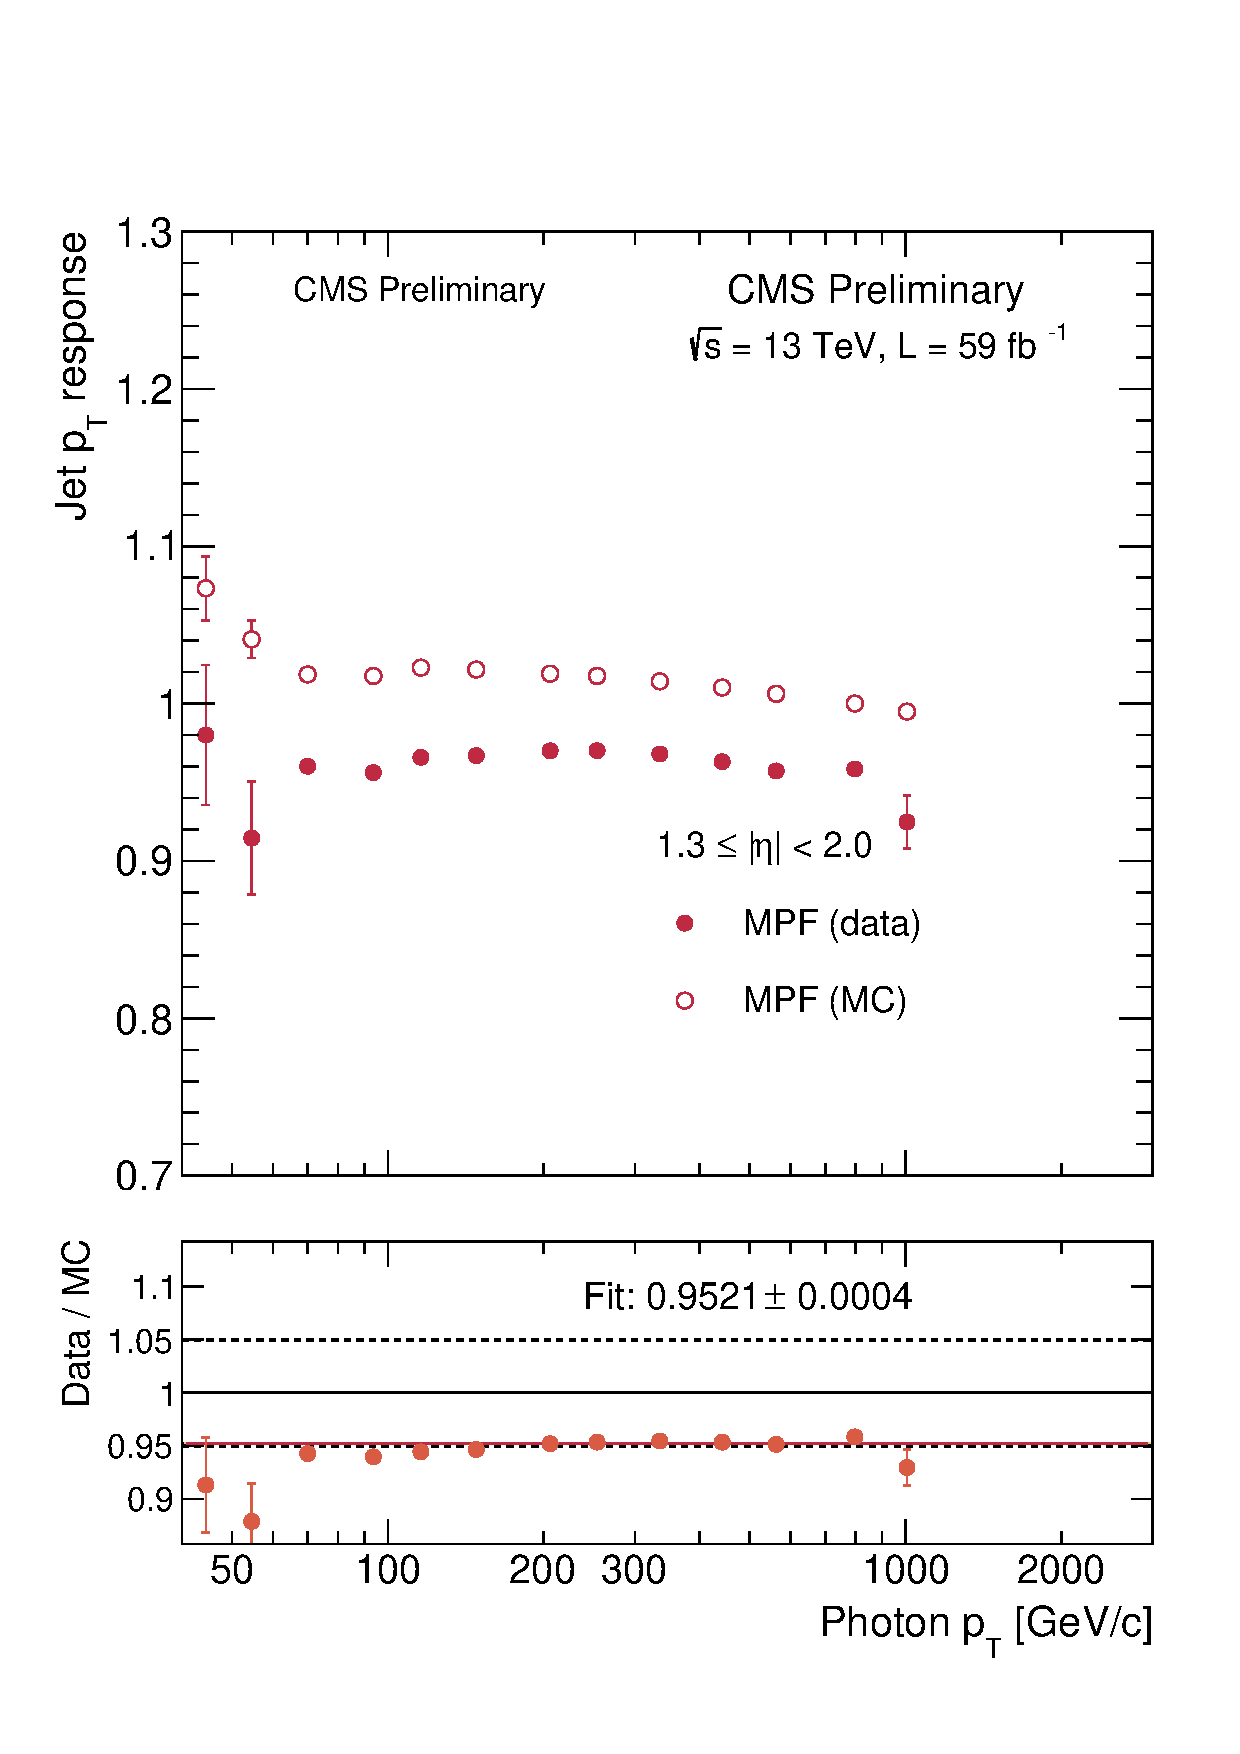
\includegraphics[width=.45\textwidth]{\PhDthesisdir/contents/chapter-JERC/plots/my_plots/only_L2Res/Run2018ABCD/alpha_0_3/response_eta1319_mpf.pdf}}

\vfill

\subcaptionbox{$\num{2.0} \leq \abs{\eta^\text{jet}} < \num{2.5}$.\label{subfig-response_eta1925_MPF_alpha_0_3_2018ABCD}}[.45\textwidth]
{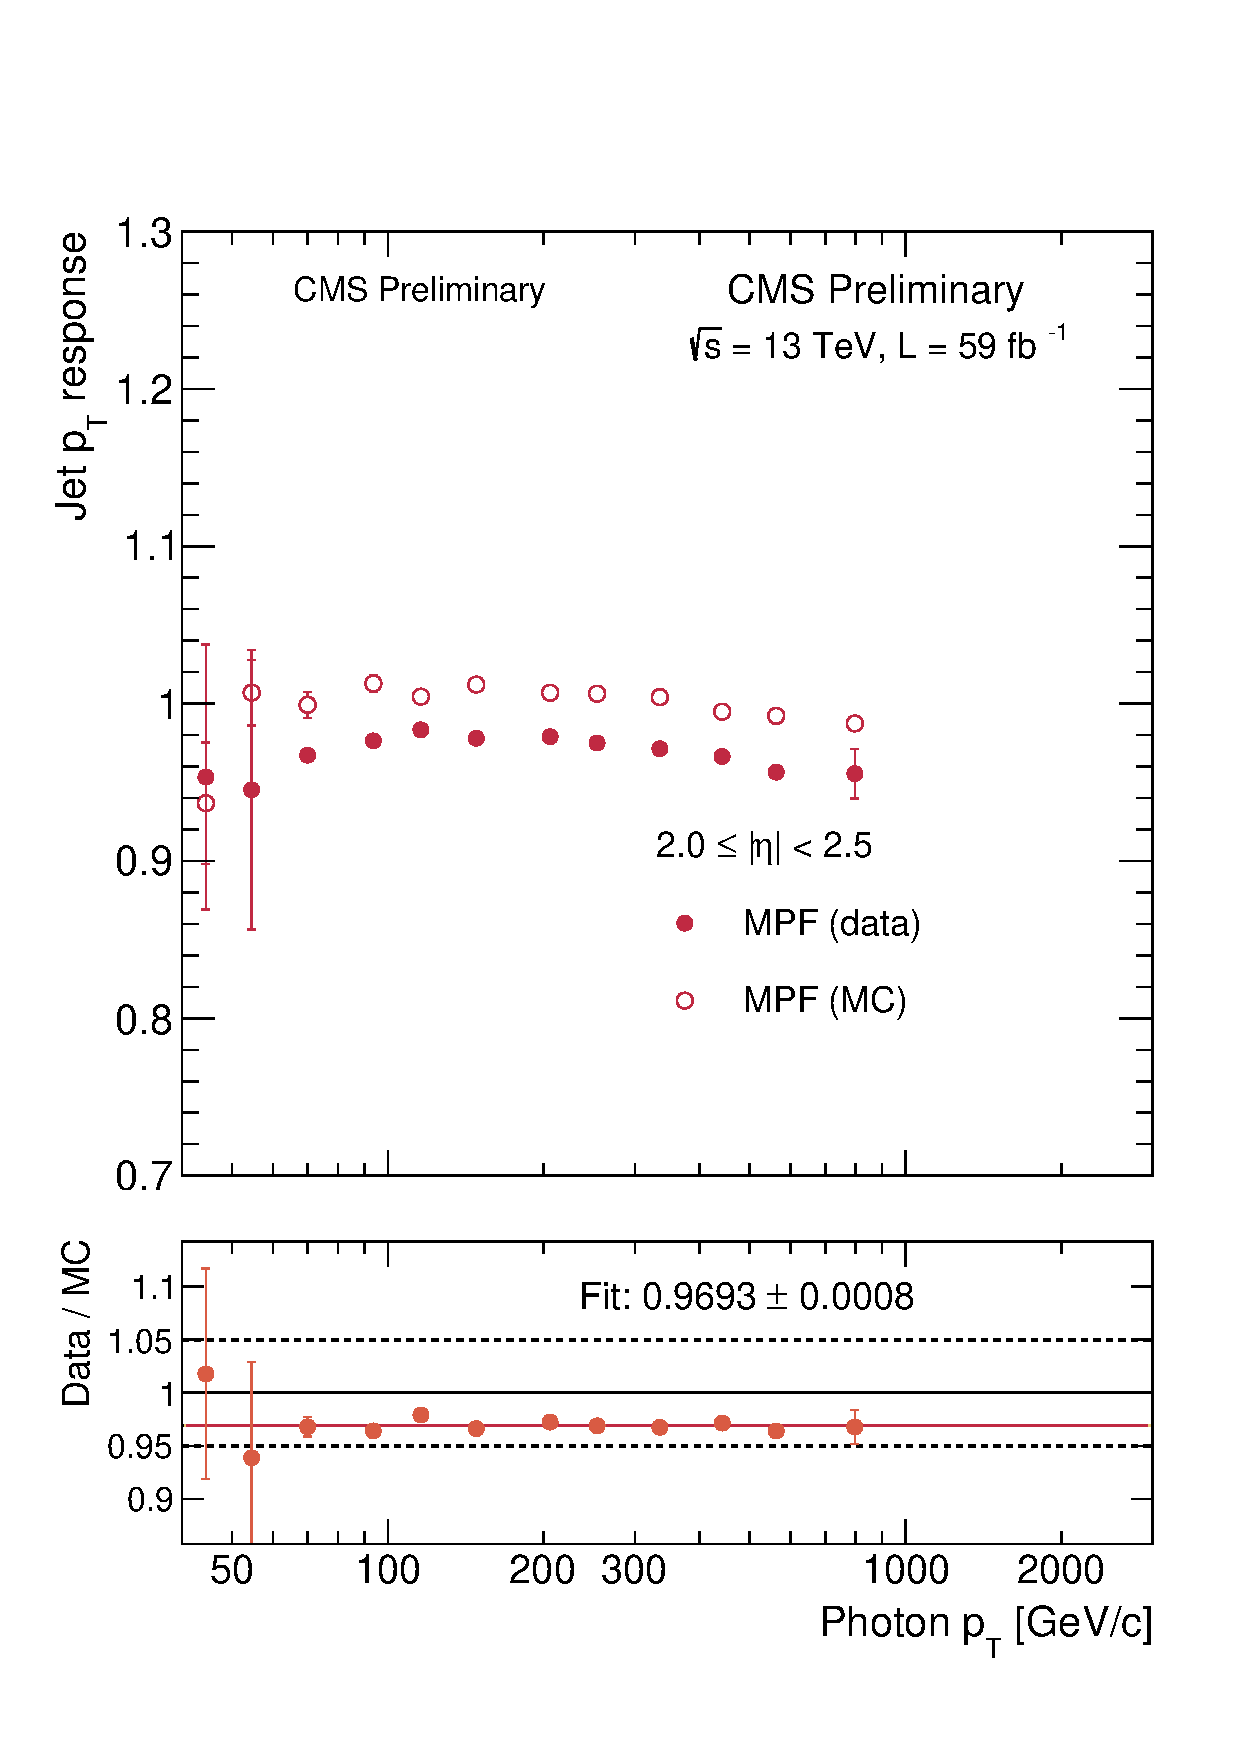
\includegraphics[width=.45\textwidth]{\PhDthesisdir/contents/chapter-JERC/plots/my_plots/only_L2Res/Run2018ABCD/alpha_0_3/response_eta1925_mpf.pdf}}
\hfill
\subcaptionbox{$\num{2.5} \leq \abs{\eta^\text{jet}} < \num{3.0}$.\label{subfig-response_eta2530_MPF_alpha_0_3_2018ABCD}}[.45\textwidth]
{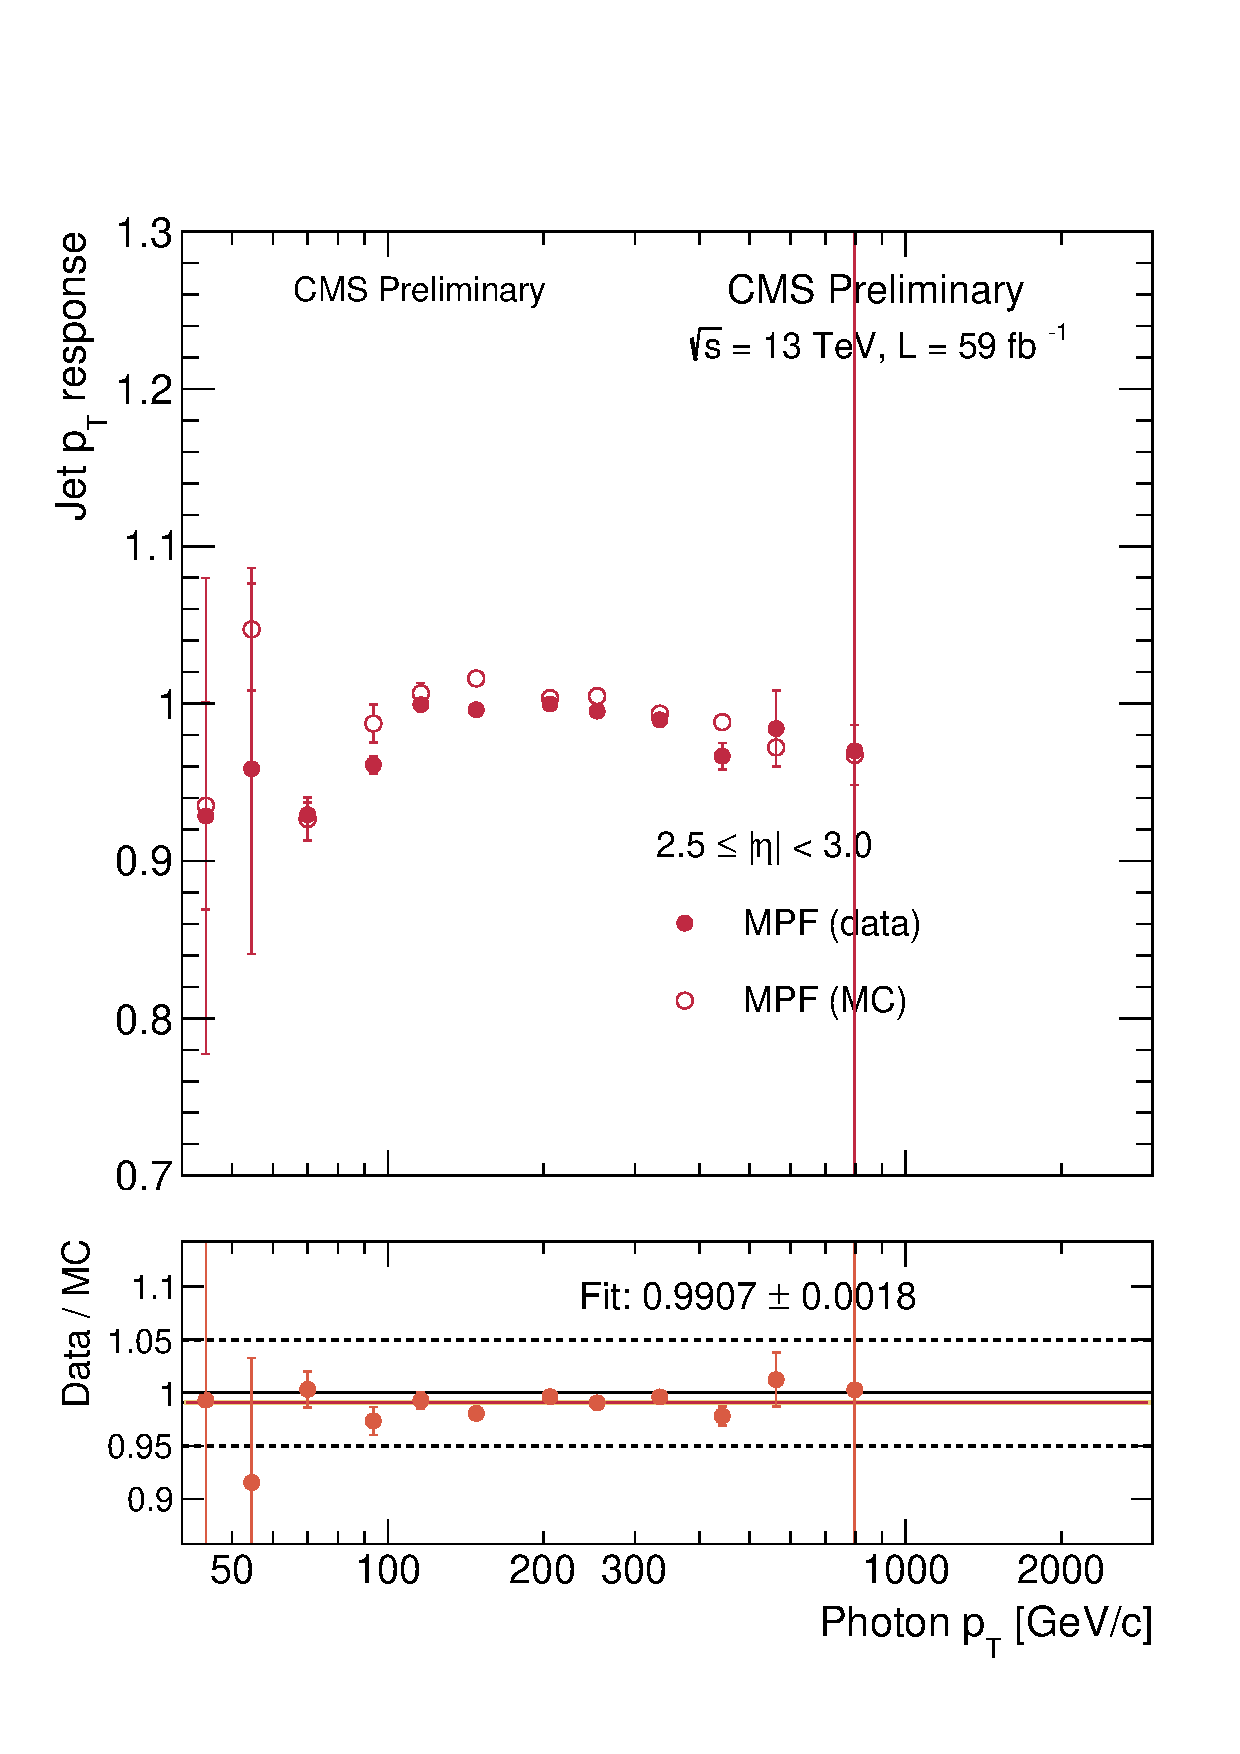
\includegraphics[width=.45\textwidth]{\PhDthesisdir/contents/chapter-JERC/plots/my_plots/only_L2Res/Run2018ABCD/alpha_0_3/response_eta2530_mpf.pdf}}

\caption[Réponses MPF en 2018 avant extrapolation.]{Distributions des réponses MPF moyennes en fonction de $\pT^{\text{\photon}}$ pour différents intervalles de $\eta^\text{jet}$ en 2018 avant extrapolation. Le rapport données sur simulations est présenté dans chaque cas ainsi qu'un ajustement à une constante donnant l'ordre de grandeur de la correction résiduelle à appliquer.}
\label{fig-responses_MPF_alpha_0_3_2018ABCD}
\end{figure}
\begin{figure}[p]
\centering
\subcaptionbox{$\abs{\eta^\text{jet}} < \num{1.3}$.\label{subfig-response_eta0013_balancing_extrapolated_2018ABCD}}[.45\textwidth]
{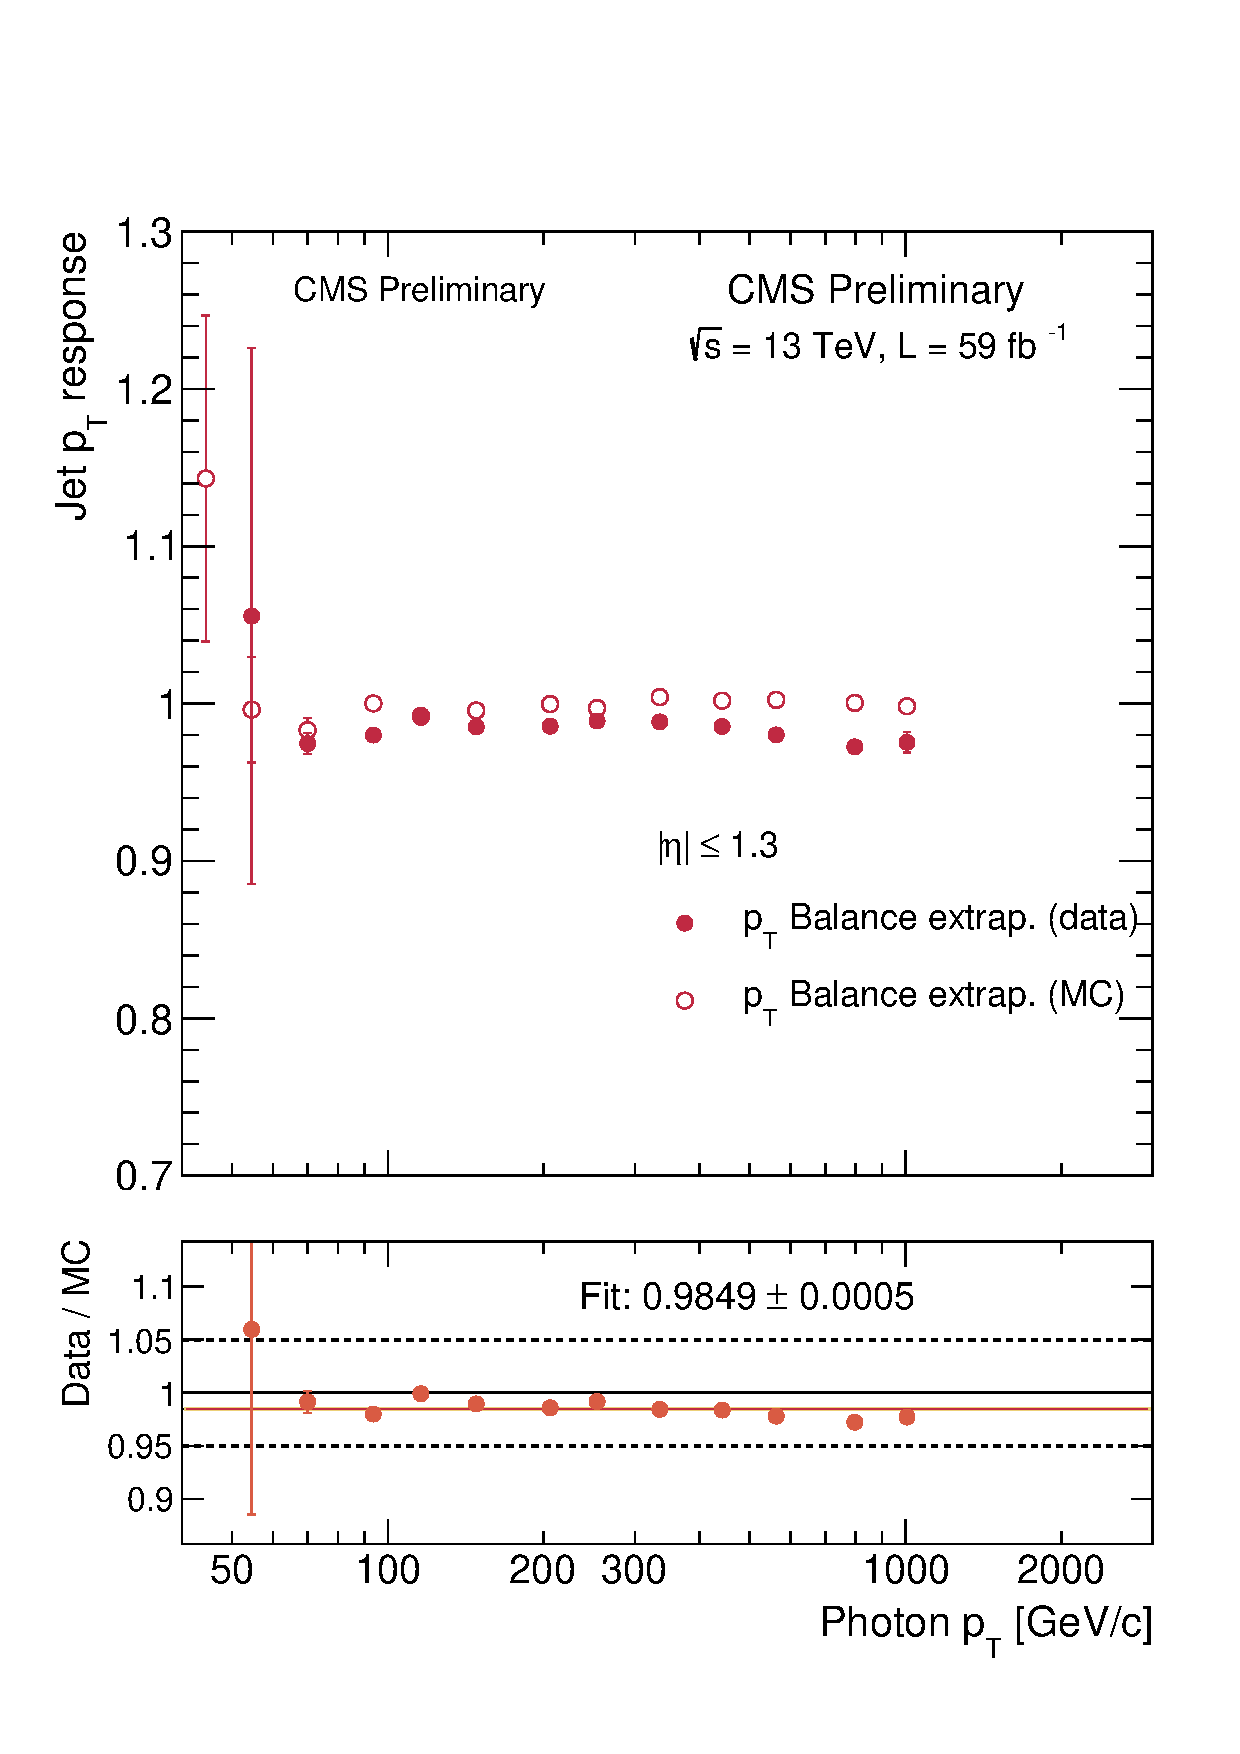
\includegraphics[width=.45\textwidth]{\PhDthesisdir/plots_and_images/my_plots/JERC/only_L2Res/Run2018ABCD/extrapolated/response_eta0013_balancing_extrap.tex}}
\hfill
\subcaptionbox{$\num{1.3} \leq \abs{\eta^\text{jet}} < \num{2.0}$.\label{subfig-response_eta1319_balancing_extrapolated_2018ABCD}}[.45\textwidth]
{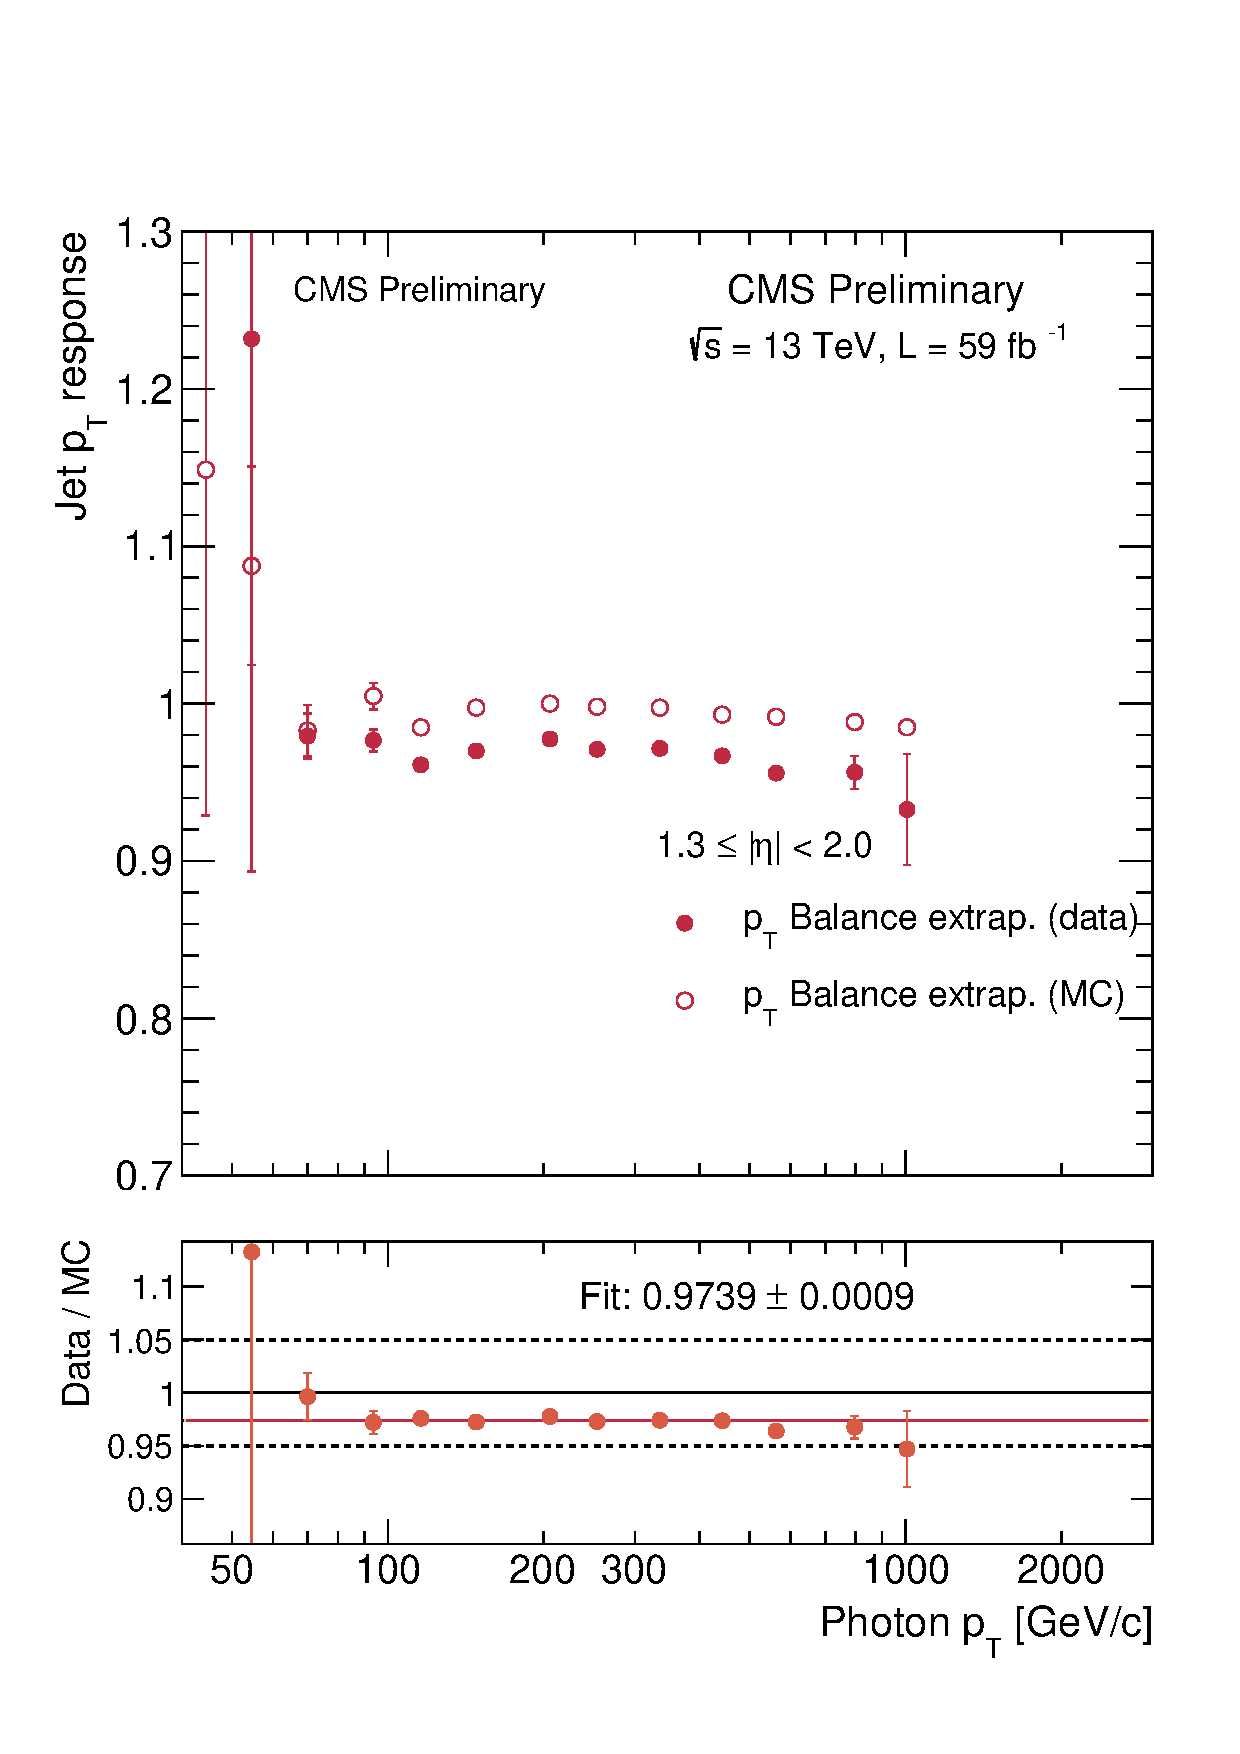
\includegraphics[width=.45\textwidth]{\PhDthesisdir/plots_and_images/my_plots/JERC/only_L2Res/Run2018ABCD/extrapolated/response_eta1319_balancing_extrap.tex}}

\vfill

\subcaptionbox{$\num{2.0} \leq \abs{\eta^\text{jet}} < \num{2.5}$.\label{subfig-response_eta1925_balancing_extrapolated_2018ABCD}}[.45\textwidth]
{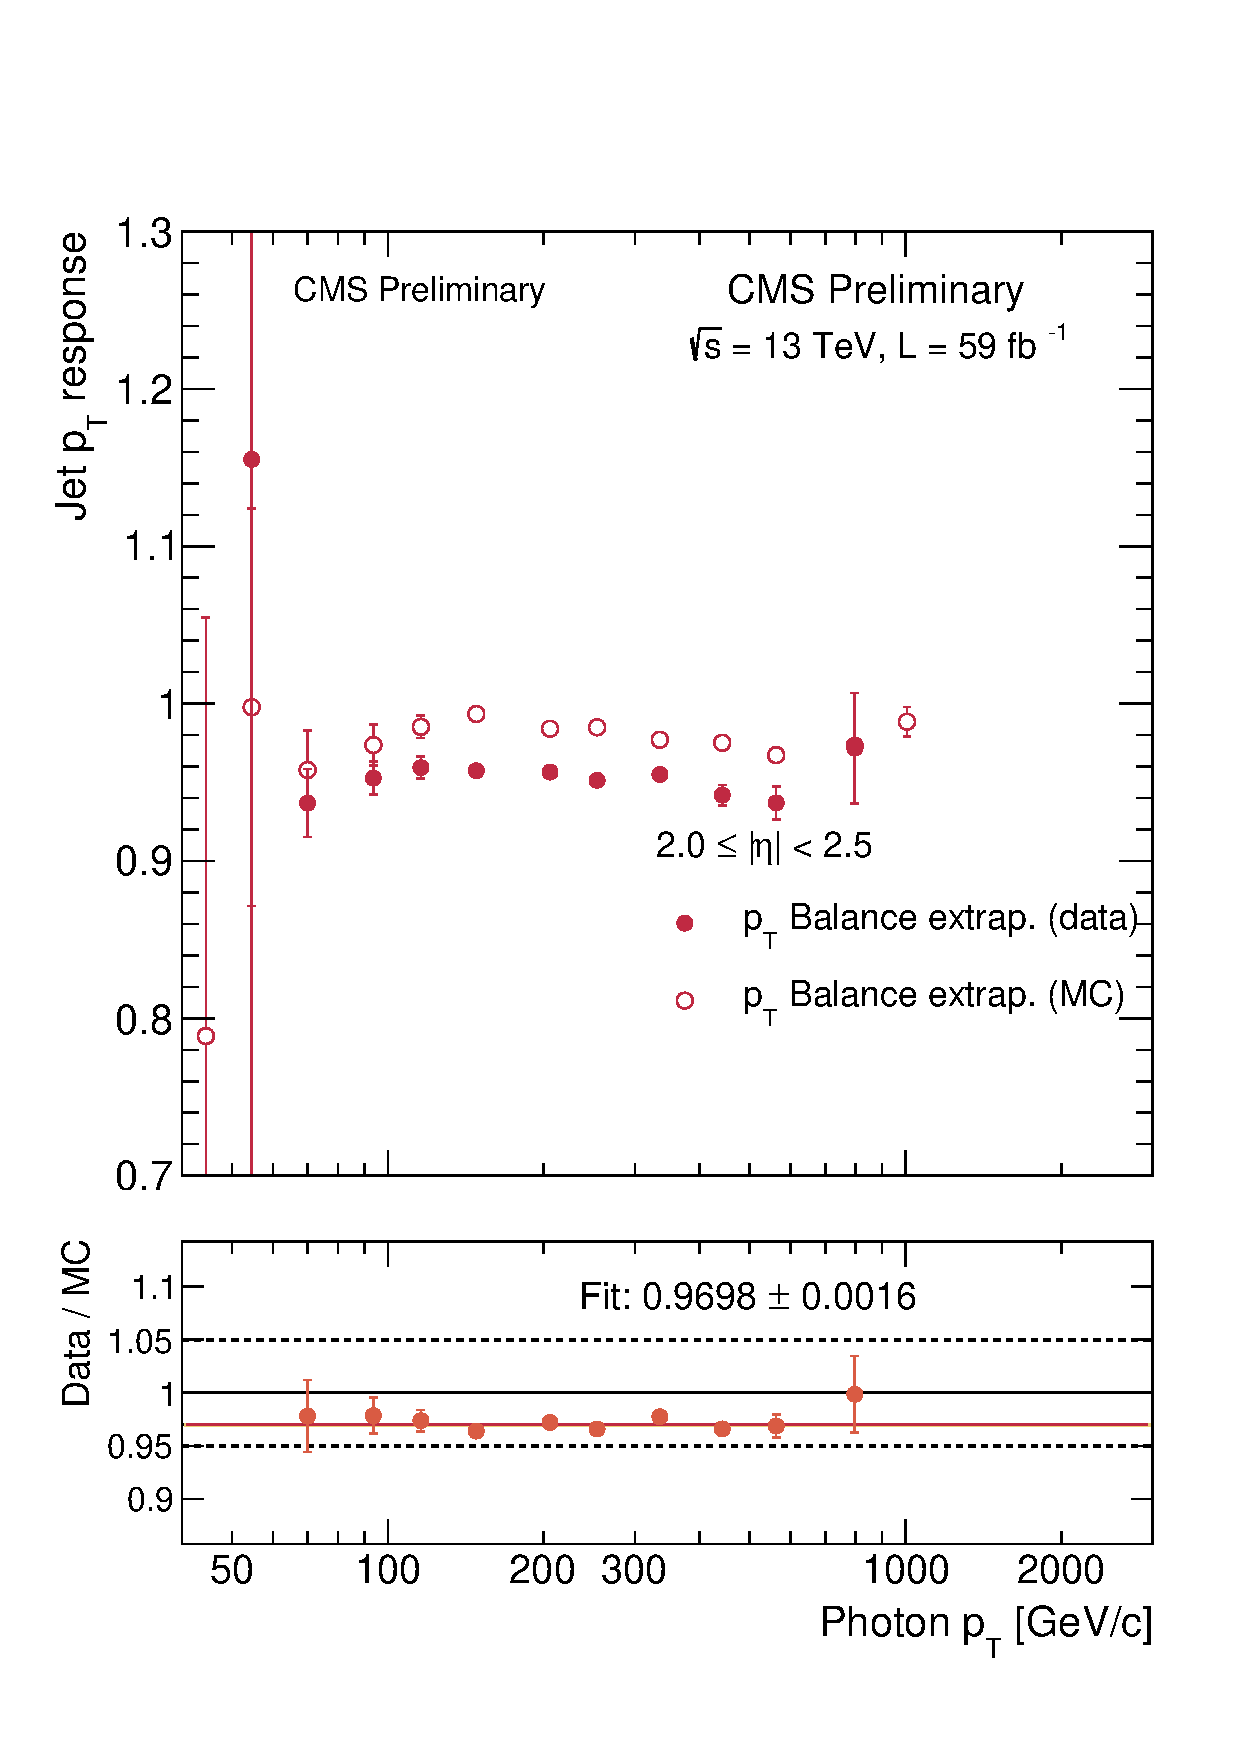
\includegraphics[width=.45\textwidth]{\PhDthesisdir/plots_and_images/my_plots/JERC/only_L2Res/Run2018ABCD/extrapolated/response_eta1925_balancing_extrap.tex}}
\hfill
\subcaptionbox{$\num{2.5} \leq \abs{\eta^\text{jet}} < \num{3.0}$.\label{subfig-response_eta2530_balancing_extrapolated_2018ABCD}}[.45\textwidth]
{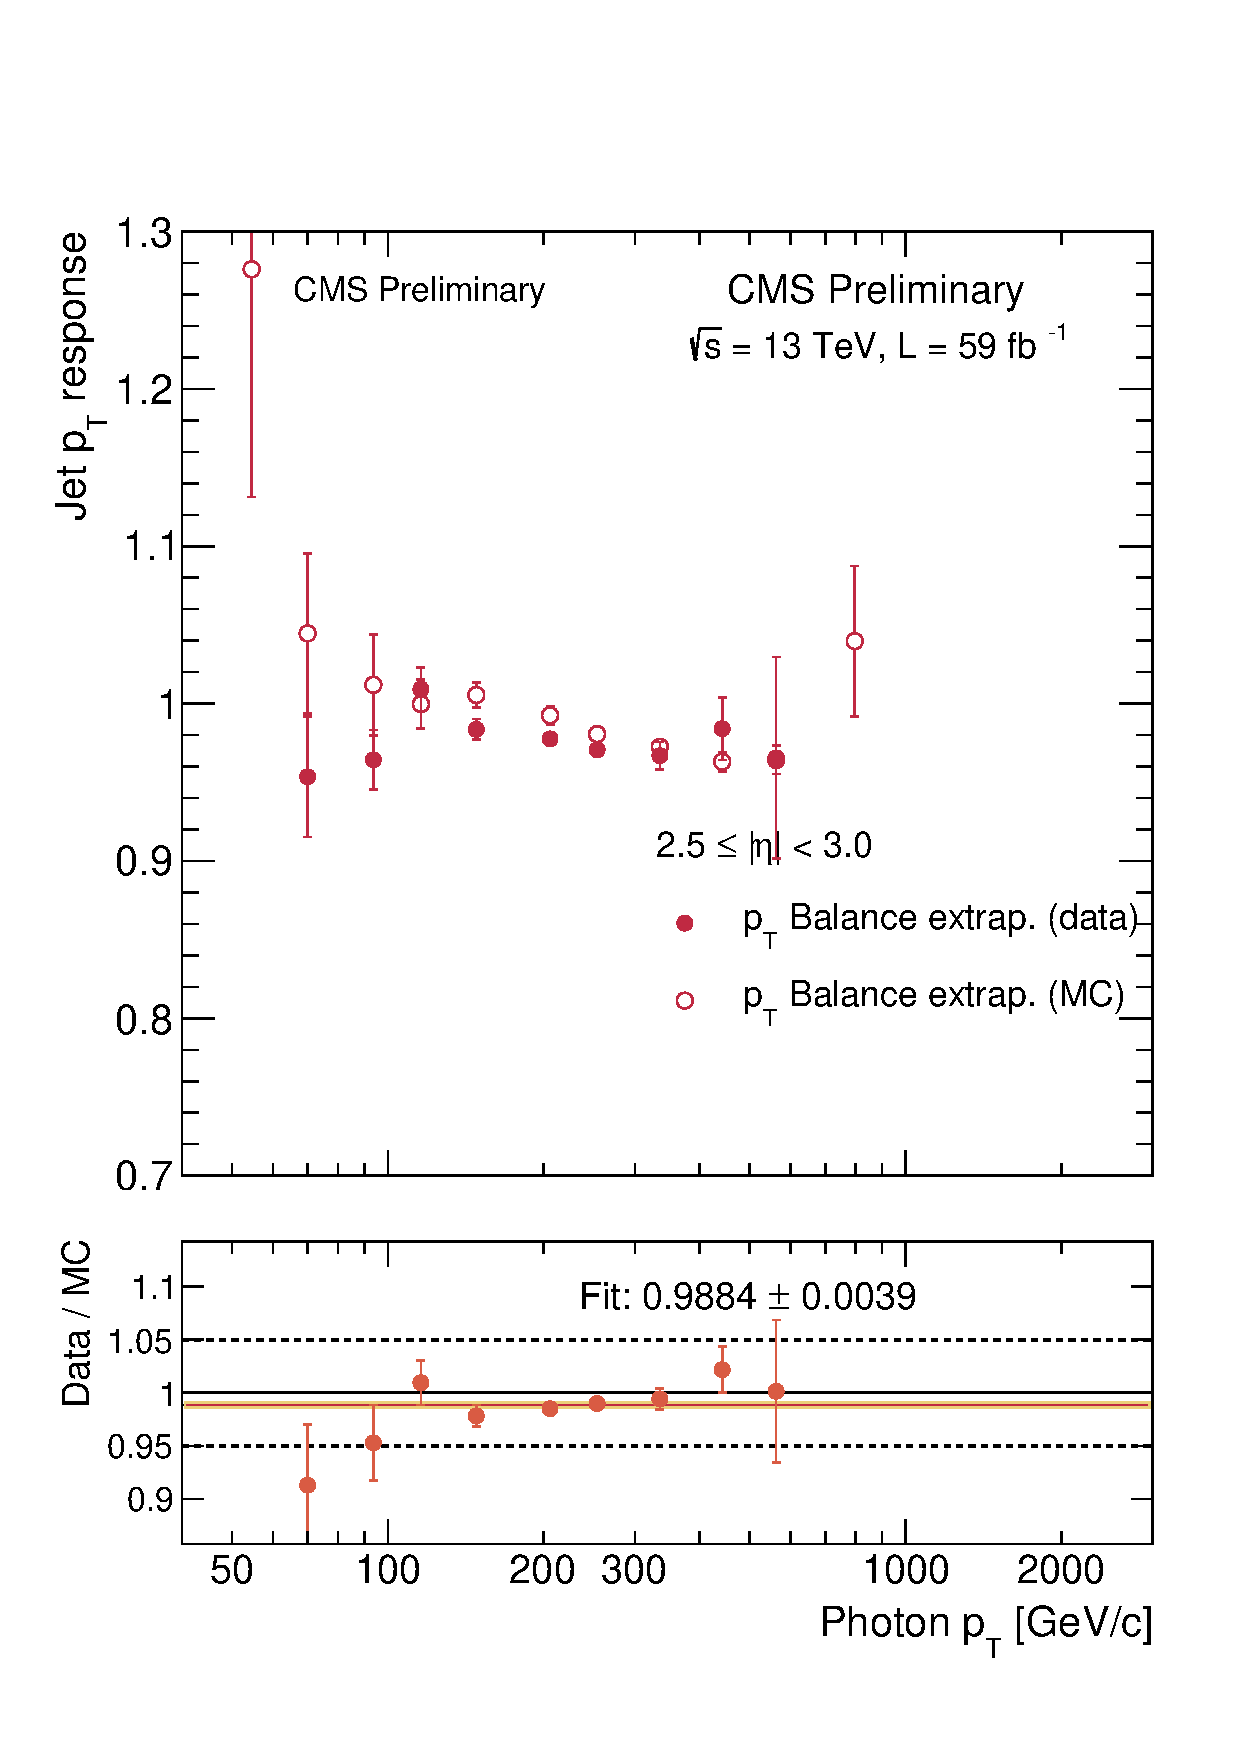
\includegraphics[width=.45\textwidth]{\PhDthesisdir/plots_and_images/my_plots/JERC/only_L2Res/Run2018ABCD/extrapolated/response_eta2530_balancing_extrap.tex}}

\caption[Réponses équilibrées en 2018 apr\`es extrapolation.]{Distributions des réponses équilibrées moyennes en fonction de $\pT^{\text{\photon}}$ pour différents intervalles de $\eta^\text{jet}$ en 2018 apr\`es extrapolation. Le rapport données réelles sur simulées est présenté dans chaque cas ainsi qu'un ajustement à une constante donnant l'ordre de grandeur de la correction résiduelle à appliquer.}
\label{fig-responses_balancing_extrapolated_2018ABCD}
\end{figure}
\begin{figure}[p]
\centering
\subcaptionbox{$\abs{\eta^\text{jet}} < \num{1.3}$.\label{subfig-response_eta0013_MPF_extrapolated_2018ABCD}}[.45\textwidth]
{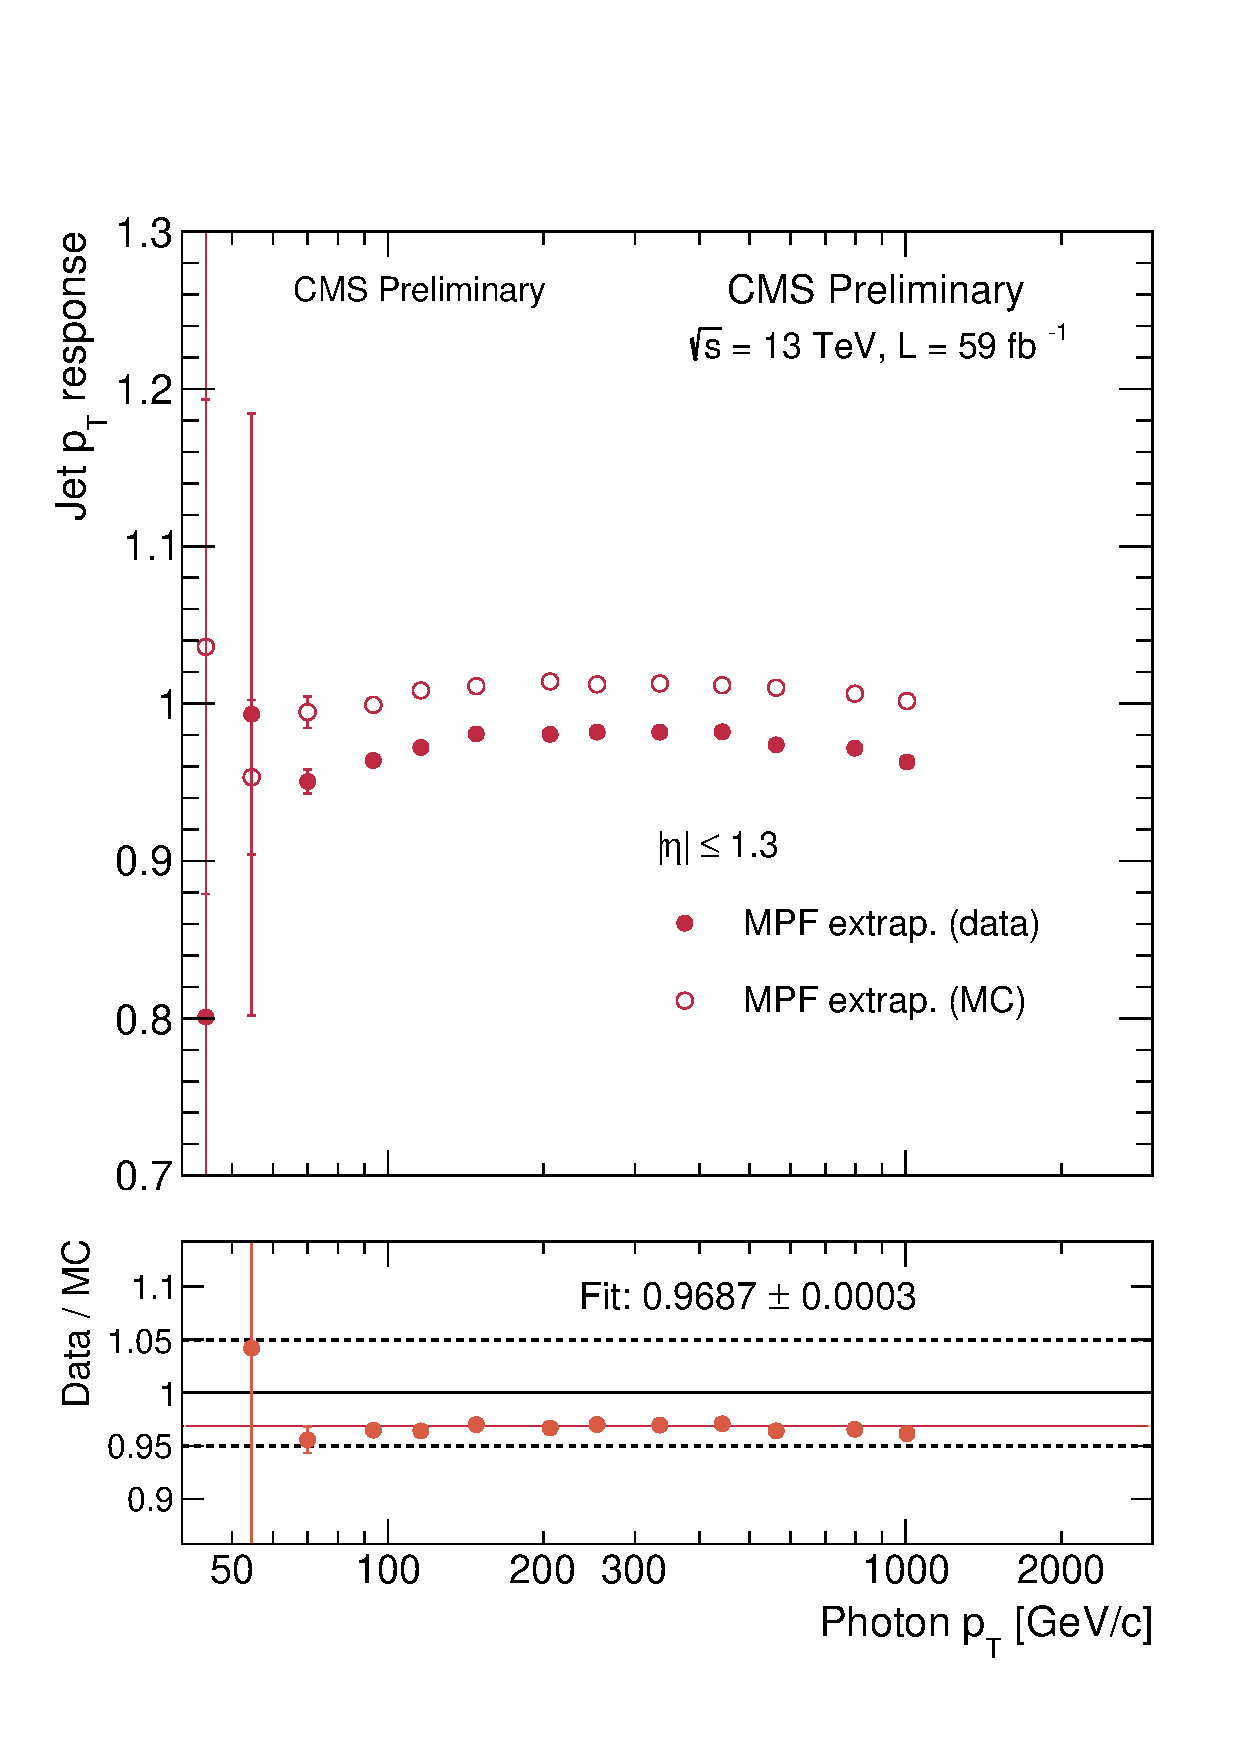
\includegraphics[width=.45\textwidth]{\PhDthesisdir/plots_and_images/my_plots/JERC/only_L2Res/Run2018ABCD/extrapolated/response_eta0013_mpf_extrap.pdf}}
\hfill
\subcaptionbox{$\num{1.3} \leq \abs{\eta^\text{jet}} < \num{2.0}$.\label{subfig-response_eta1319_MPF_extrapolated_2018ABCD}}[.45\textwidth]
{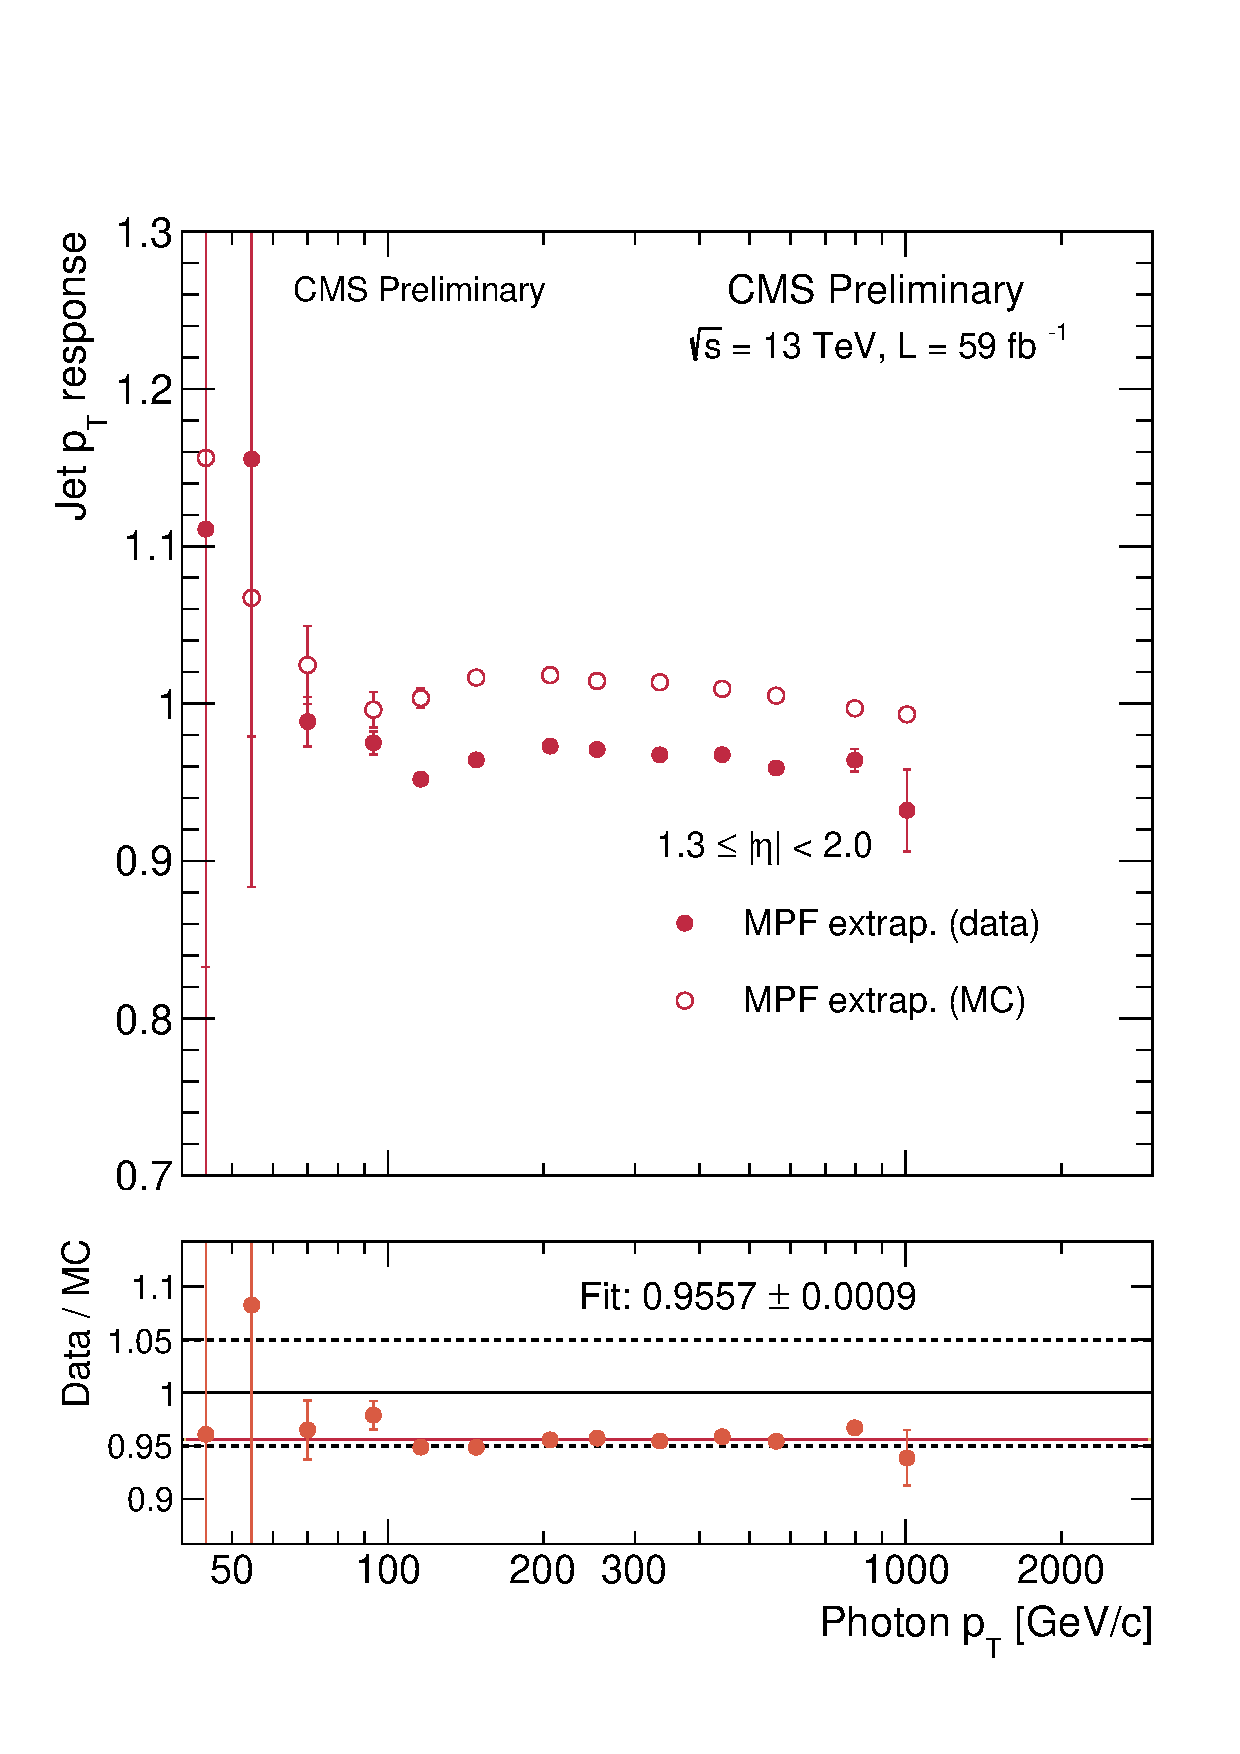
\includegraphics[width=.45\textwidth]{\PhDthesisdir/plots_and_images/my_plots/JERC/only_L2Res/Run2018ABCD/extrapolated/response_eta1319_mpf_extrap.pdf}}

\vfill

\subcaptionbox{$\num{2.0} \leq \abs{\eta^\text{jet}} < \num{2.5}$.\label{subfig-response_eta1925_MPF_extrapolated_2018ABCD}}[.45\textwidth]
{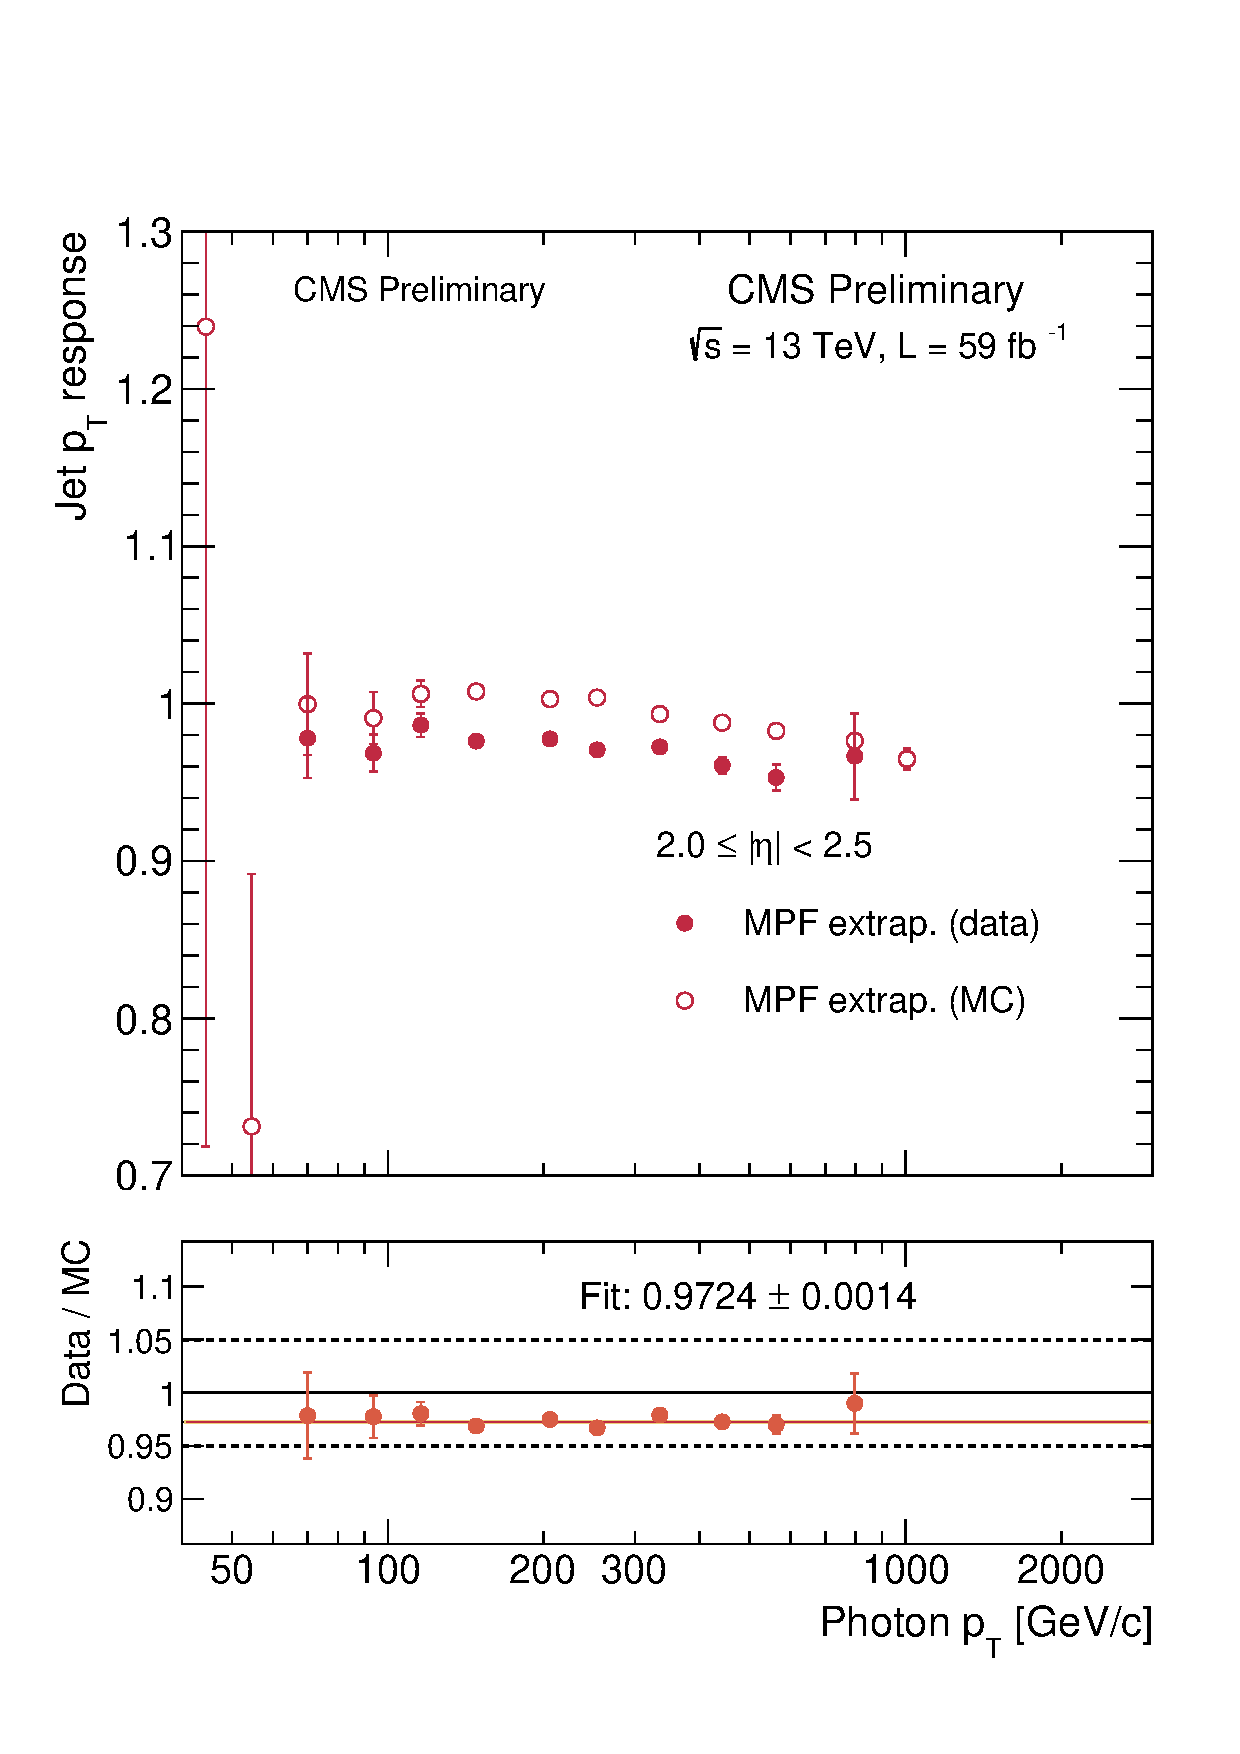
\includegraphics[width=.45\textwidth]{\PhDthesisdir/plots_and_images/my_plots/JERC/only_L2Res/Run2018ABCD/extrapolated/response_eta1925_mpf_extrap.pdf}}
\hfill
\subcaptionbox{$\num{2.5} \leq \abs{\eta^\text{jet}} < \num{3.0}$.\label{subfig-response_eta2530_MPF_extrapolated_2018ABCD}}[.45\textwidth]
{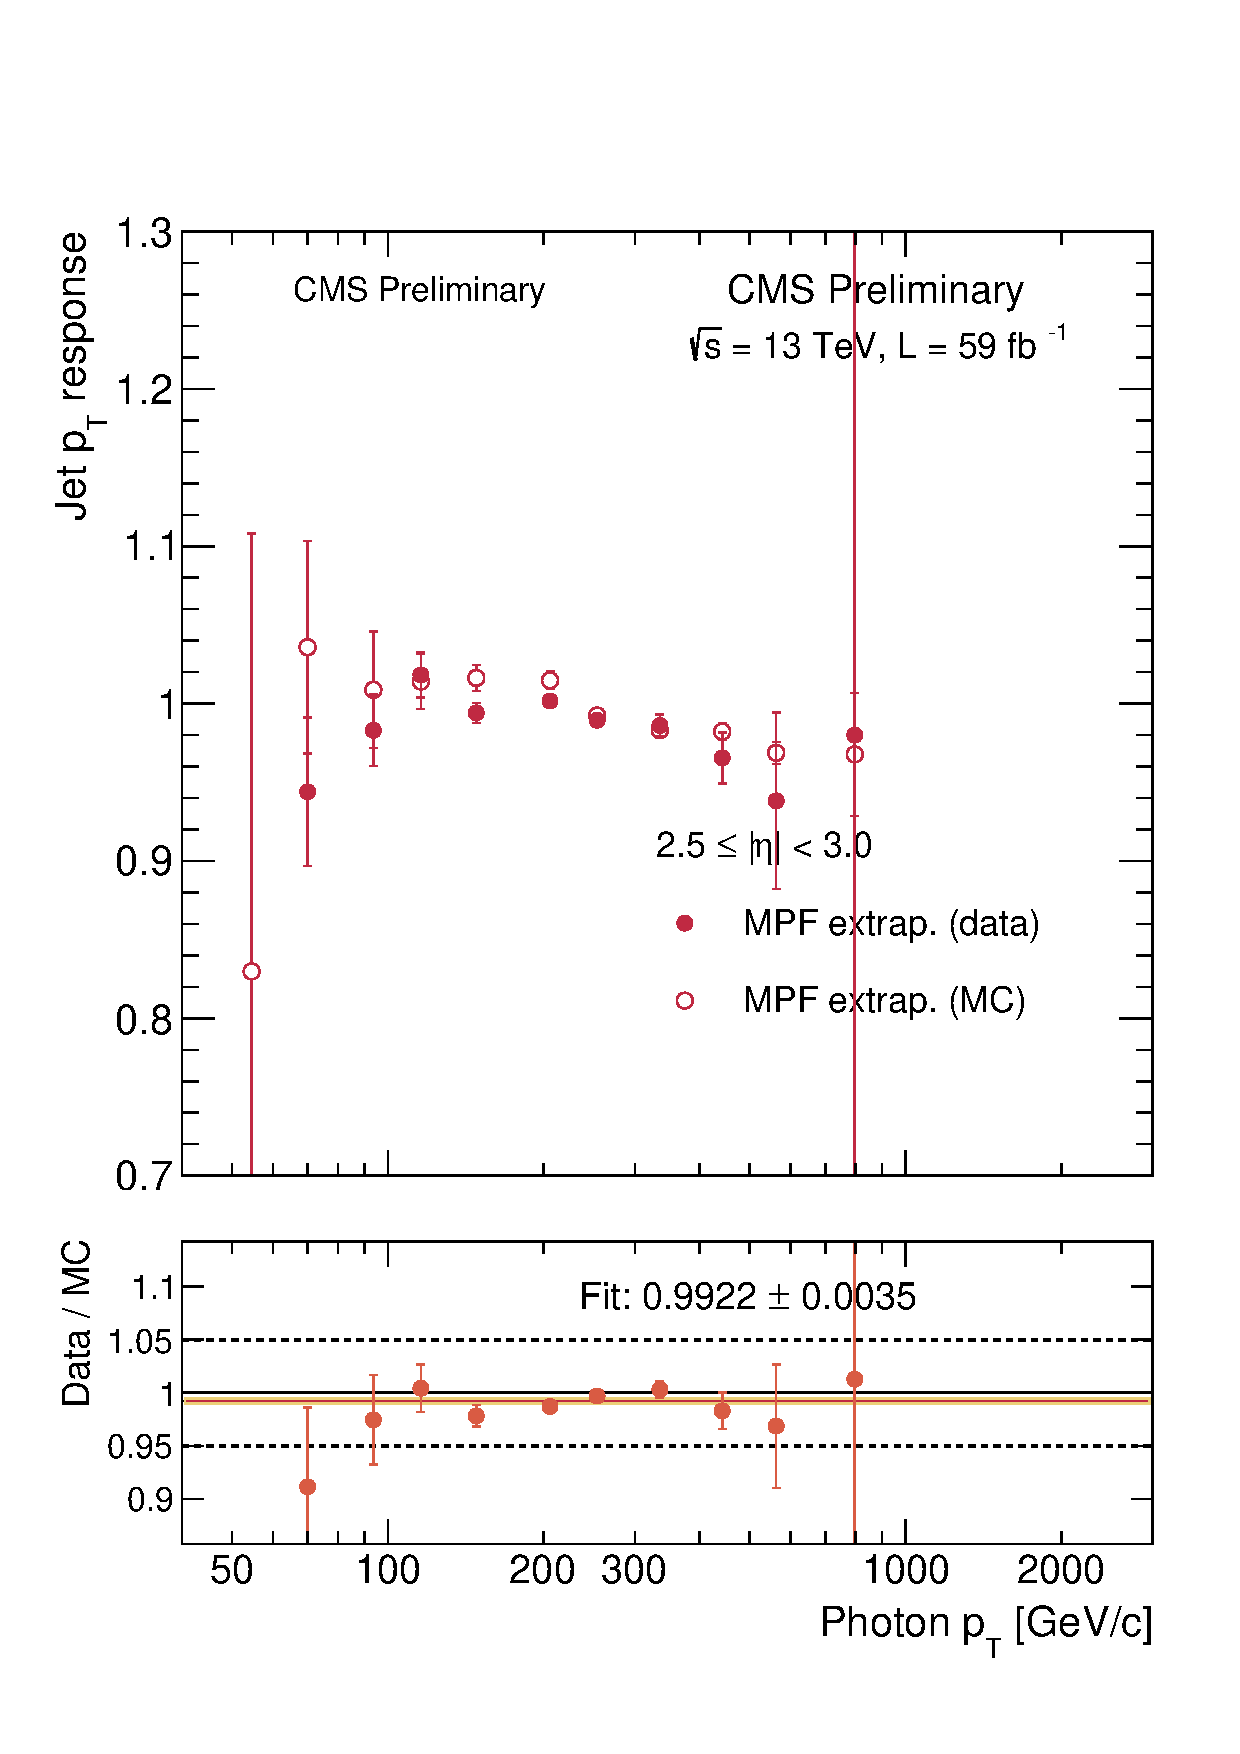
\includegraphics[width=.45\textwidth]{\PhDthesisdir/plots_and_images/my_plots/JERC/only_L2Res/Run2018ABCD/extrapolated/response_eta2530_mpf_extrap.pdf}}

\caption[Réponses MPF en 2018 apr\`es extrapolation.]{Distributions des réponses MPF moyennes en fonction de $\pT^{\text{\photon}}$ pour différents intervalles de $\eta^\text{jet}$ en 2018 apr\`es extrapolation. Le rapport données sur simulations est présenté dans chaque cas ainsi qu'un ajustement à une constante donnant l'ordre de grandeur de la correction résiduelle à appliquer.}
\label{fig-responses_MPF_extrapolated_2018ABCD}
\end{figure}

\subsubsection{Ajustement global}\label{chapter-JERC-section-JES-subsec-results-subsubsec-global_fit}
Les événements \Gjets\ ne permettent pas à eux seuls de couvrir avec une statistique suffisante l'ensemble de la gamme d'impulsions transverses à calibrer.
De plus, l'utilisation de différentes catégories d'événements permet de valider \aposteriori\ les résultats des analyses entre elles.
Un ajustement global est alors réalisé sur les événements \Zjets, \Gjets\ et multijet afin d'obtenir la correction finale à appliquer aux données.
\par Cet ajustement est réalisé en minimisant un $\chi^2$ prenant en compte les contraintes de chaque catégorie d'événements.
La correction résiduelle absolue en \pT\ des jets correspond ainsi à l'ajustement d'une fonction paramétrique.
Les incertitudes présentes dans les différentes analyses sont considérées comme des paramètres de nuisance pour l'ajustement. Ces incertitudes sont:
\begin{itemize}
\item \SI{4.6}{\%} sur la section efficace de collision inélastique \proton\proton\ utilisée pour estimer les profils d'empilement;
\item les incertitudes de la JEC, décrites section~\ref{chapter-JERC-section-CMS-subsec-unc}, page~\pageref{chapter-JERC-section-CMS-subsec-unc};
\item l'échelle en énergie des objets de référence, \SI{0.2}{\%} pour les photons et les muons, \SI{0.5}{\%} pour les électrons;
\item les effets de l'ISR et du FSR se retrouvant dans l'incertitude de l'extrapolation en $\alpha$;
\item la propagation des calibrations des photons et des électrons dans l'énergie transverse manquante.
\end{itemize}
\par La figure~\ref{fig-chapter-JERC-section-JES-subsec-results-response_eta0013_alpha_0_3_2018} compare les résultats produits lors de ma thèse avec les événements \Gjets\ à ceux de l'analyse basée sur les événements \Zmmjets\ pour l'année 2018.
La réponse des jets dans les données diminue du Run~A au Run~D dans les deux analyses, ce qui est dû à l'évolution des conditions d'acquisition des données au cours du temps.
Le vieillissement du détecteur est une des sources de dépendance temporelle de la réponse des jets.
La calibration en énergie des jets est ainsi déterminée à la fois pour une année entière, pour les différents \emph{runs} individuellement et éventuellement pour des ensembles de \emph{runs} successifs, ce qui permet d'améliorer la précision obtenue sur l'énergie des jets.
\begin{figure}[h]
\centering
\subcaptionbox{Avec les événements \Gjets.\label{subfig-chapter-JERC-section-JES-subsec-results-response_eta0013_alpha_0_3_Gjets_2018}}[.45\textwidth]
{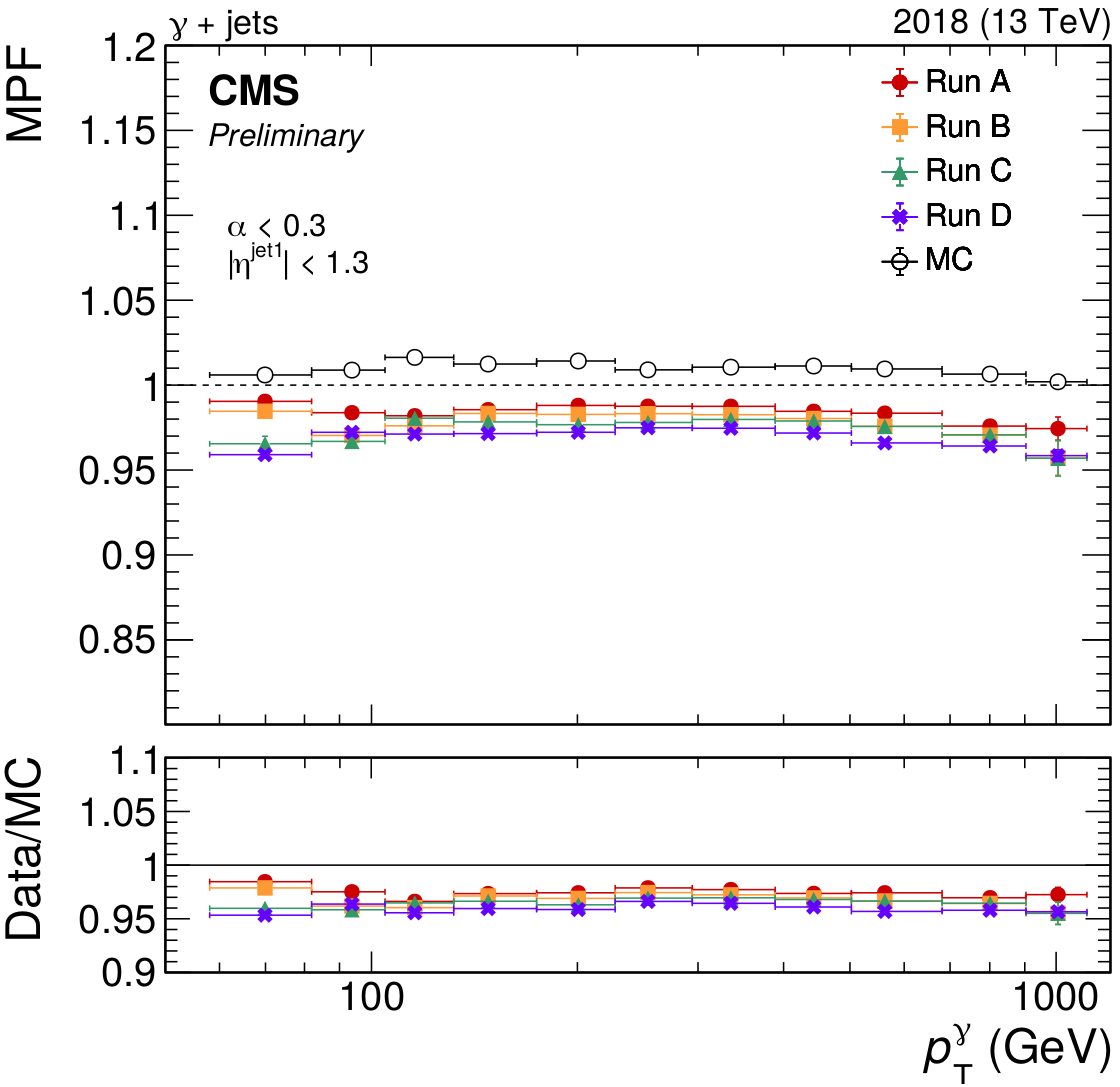
\includegraphics[width=.45\textwidth]{\PhDthesisdir/plots_and_images/from_CMS-DP-2020-019/MPF_response_Run2018_alpha_0_3_in_Gjets.png}}
\hfill
\subcaptionbox{Avec les événements \Zmmjets.\label{subfig-chapter-JERC-section-JES-subsec-results-response_eta0013_alpha_0_3_Zmmjets_2018}}[.45\textwidth]
{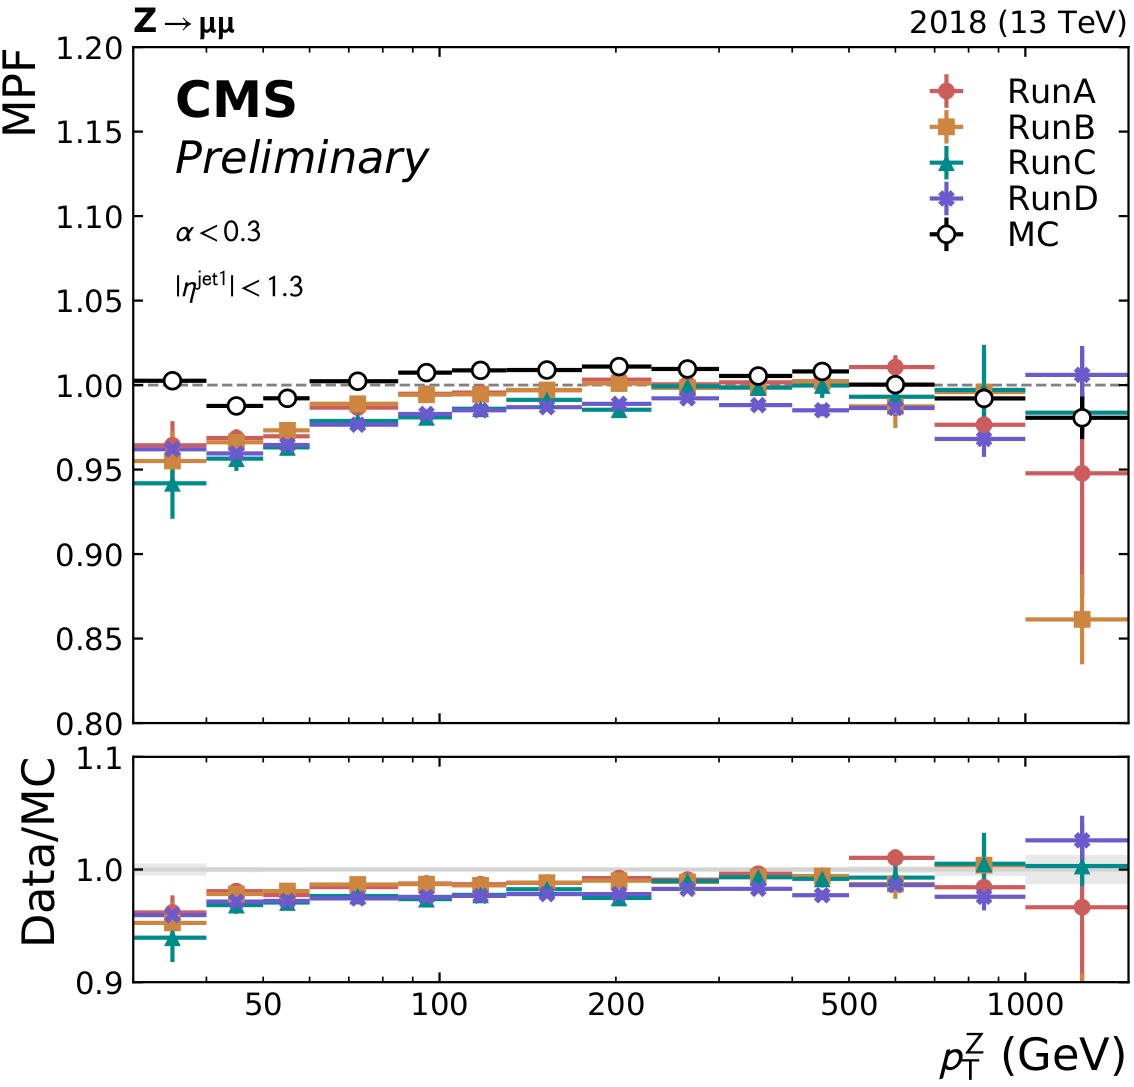
\includegraphics[width=.45\textwidth]{\PhDthesisdir/plots_and_images/from_CMS-DP-2020-019/MPF_response_Run2018_alpha_0_3_in_Zmmjets.png}}
\caption[Distributions de la réponse MPF moyenne en fonction de \pT\ en 2018.]{Distributions de la réponse MPF moyenne en fonction de \pT\ dans les événements avec $\abs{\eta^\text{jet}}<\num{1.3}$ et $\alpha<\num{0.3}$ pour chaque période de prise de données et pour les simulations en 2018~\cite{CMS-DP-2020-019}.}
\label{fig-chapter-JERC-section-JES-subsec-results-response_eta0013_alpha_0_3_2018}
\end{figure}
\par L'ajustement global sur les résultats des différentes analyses est illustré, pour les trois années du Run~II, sur la figure~\ref{fig-L3ResAbs_RunII} en page~\pageref{fig-L3ResAbs_RunII}.
La correction résiduelle absolue en \pT\ des jets utilisée par la collaboration CMS est ainsi obtenue.
\subsubsection{Test d'intégrité}\label{chapter-JERC-section-JES-subsec-results-subsubsec-L2L3Res_cross_check}
Il est possible de vérifier que la correction résiduelle absolue en \pT\ des jets déterminée permet bien de rapprocher les réponses des jets entre données et simulations.
Pour cela, l'analyse est à nouveau réalisée en appliquant la correction résiduelle absolue en \pT\ des jets lors de leur calibration.
Les valeurs des rapports données sur simulations des réponses balancée et MPF obtenus avant et après utilisation de cette correction sont présentés dans le tableau~\ref{tab-responses_recap_table_L2L3Res_cross_check_2018ABCD}. Ces rapports se rapprochent de \num{1}, ce qui montre que la correction améliore l'accord données-simulations.
Cette amélioration peut également se constater sur les distributions des réponses des jets, dont une comparaison est proposée sur la figure~\ref{fig-distribs_Gjets_18_resp_mpf_L2L3Res_cross_check} où les deux distributions sont plus proches l'une de l'autre après correction complète.
\begin{table}[p]
\centering
\begin{tabular}{lcccc}
\toprule
\multirow{2}{*}{$\abs{\eta^\text{jet}}\in$} & \multicolumn{2}{c}{Réponse balancée} & \multicolumn{2}{c}{Réponse MPF} \\
\cmidrule(lr){2-3}\cmidrule(lr){4-5}
 & avant $\mathcal{C}_\text{Res}$ & après $\mathcal{C}_\text{Res}$ & avant $\mathcal{C}_\text{Res}$ & après $\mathcal{C}_\text{Res}$ \\
\midrule
$[\num{0}\isp \num{1.3}[$ & $\num{0.9669}\pm\num{0.0004}$ & $\num{0.9867}\pm\num{0.0004}$ & $\num{0.9687}\pm\num{0.0003}$ & $\num{0.9877}\pm\num{0.0003}$ \\
$[\num{1.3}\isp \num{2.0}[$ & $\num{0.9538}\pm\num{0.0009}$ & $\num{0.9739}\pm\num{0.0009}$ & $\num{0.9565}\pm\num{0.0008}$ & $\num{0.9753}\pm\num{0.0008}$ \\
$[\num{2.0}\isp \num{2.5}[$ & $\num{0.9502}\pm\num{0.0015}$ & $\num{0.9698}\pm\num{0.0016}$ & $\num{0.9516}\pm\num{0.0014}$ & $\num{0.9724}\pm\num{0.0014}$ \\
$[\num{2.5}\isp \num{3.0}[$ & $\num{0.9661}\pm\num{0.0037}$ & $\num{0.9884}\pm\num{0.0039}$ & $\num{0.9707}\pm\num{0.0034}$ & $\num{0.9922}\pm\num{0.0035}$ \\
\bottomrule
\end{tabular}
\caption[Rapports des réponses balancée et MPF obtenus en 2018 après extrapolation vers $\alpha=0$.]{Rapports données réelles sur simulées des réponses balancée et MPF obtenus en 2018 après extrapolation vers $\alpha=0$.}
\label{tab-responses_recap_table_L2L3Res_cross_check_2018ABCD}
\end{table}
\begin{figure}[h]
\centering
\subcaptionbox{Avant correction (figure~\ref{subfig-distrib_Gjets_18_resp_mpf_eta0013_ptPhot_175_230}).\label{subfig-distrib_Gjets_18_resp_mpf_eta0013_ptPhot_175_230_only_L2Res}}[.45\textwidth]
{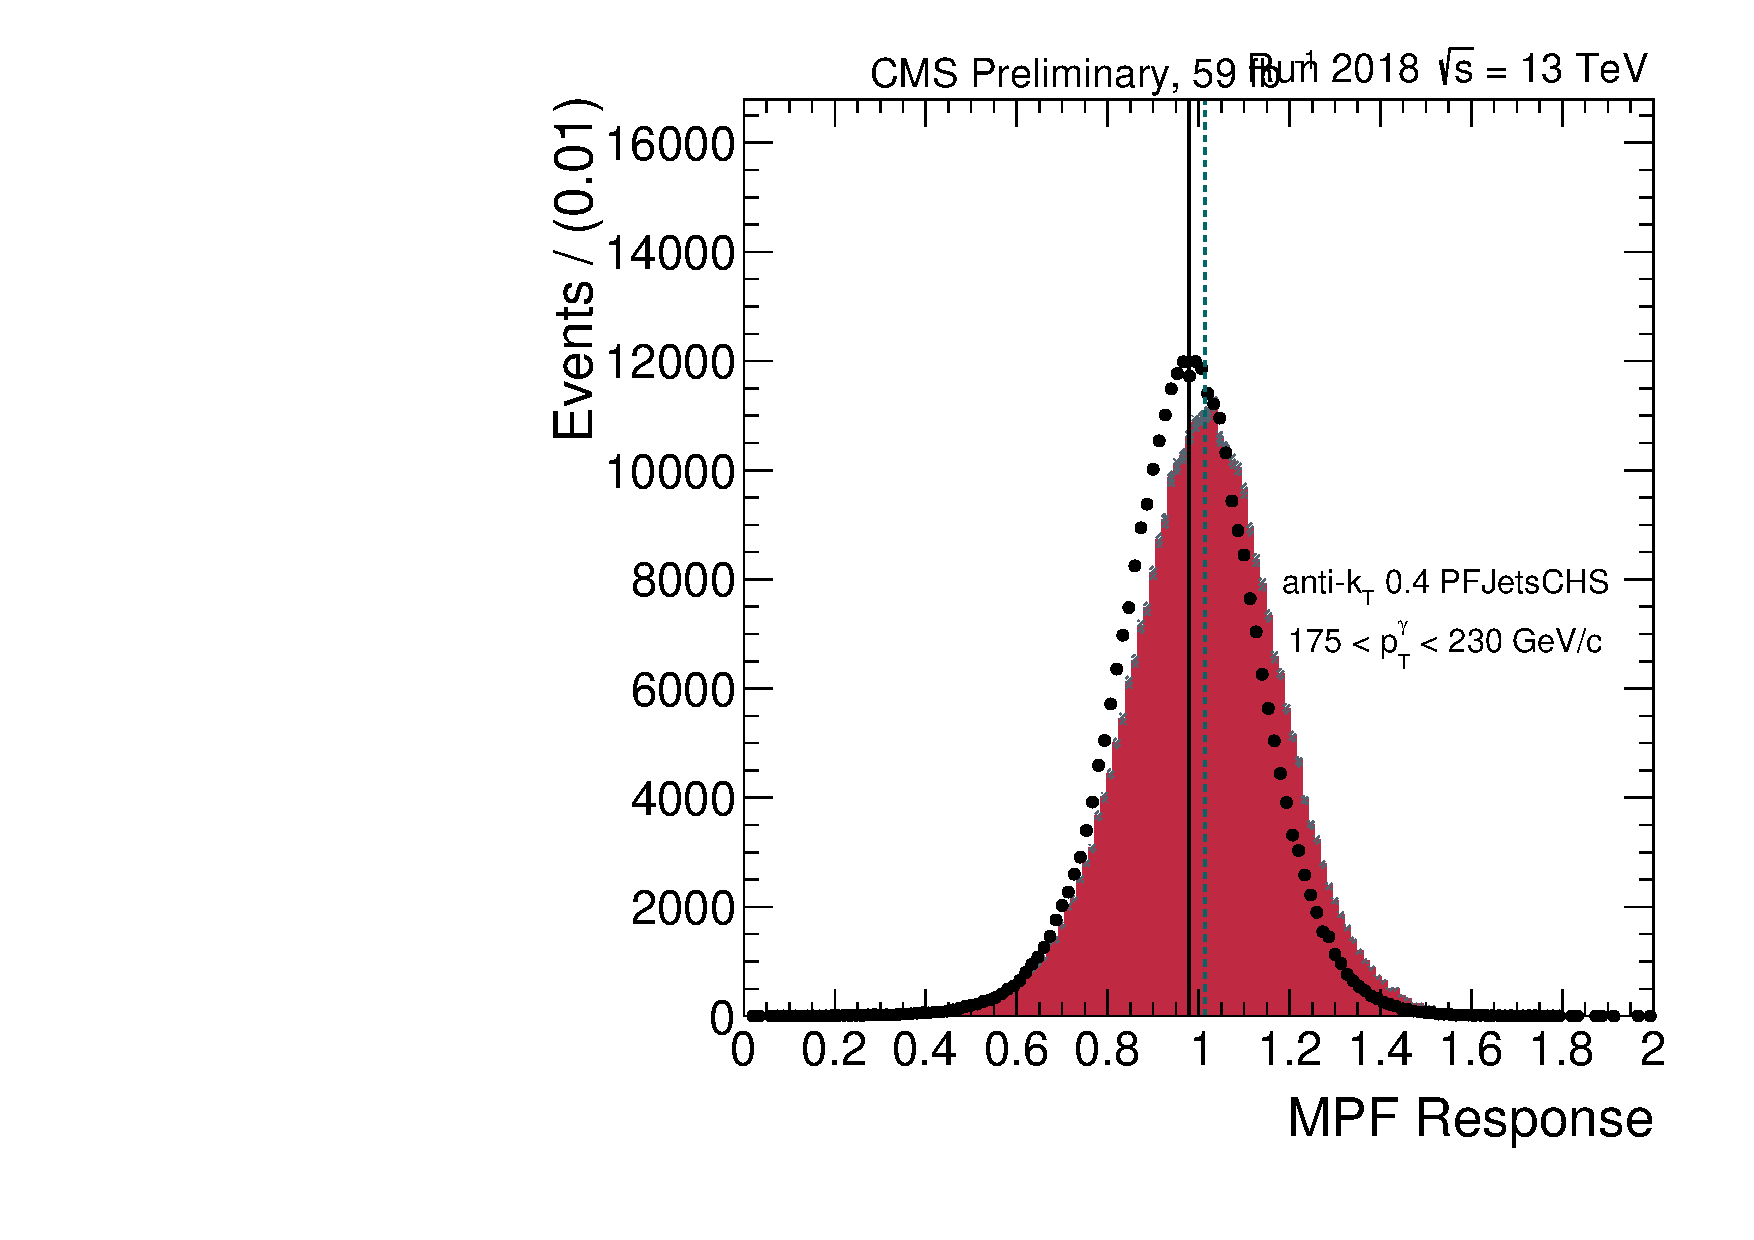
\includegraphics[width=.45\textwidth]{\PhDthesisdir/plots_and_images/my_plots/JERC/distributions/2018/with_header/resp_mpf_eta0013_ptPhot_175_230.tex}}
\hfill
\subcaptionbox{Après correction.\label{subfig-distrib_Gjets_18_resp_mpf_eta0013_ptPhot_175_230_L2L3Res}}[.45\textwidth]
{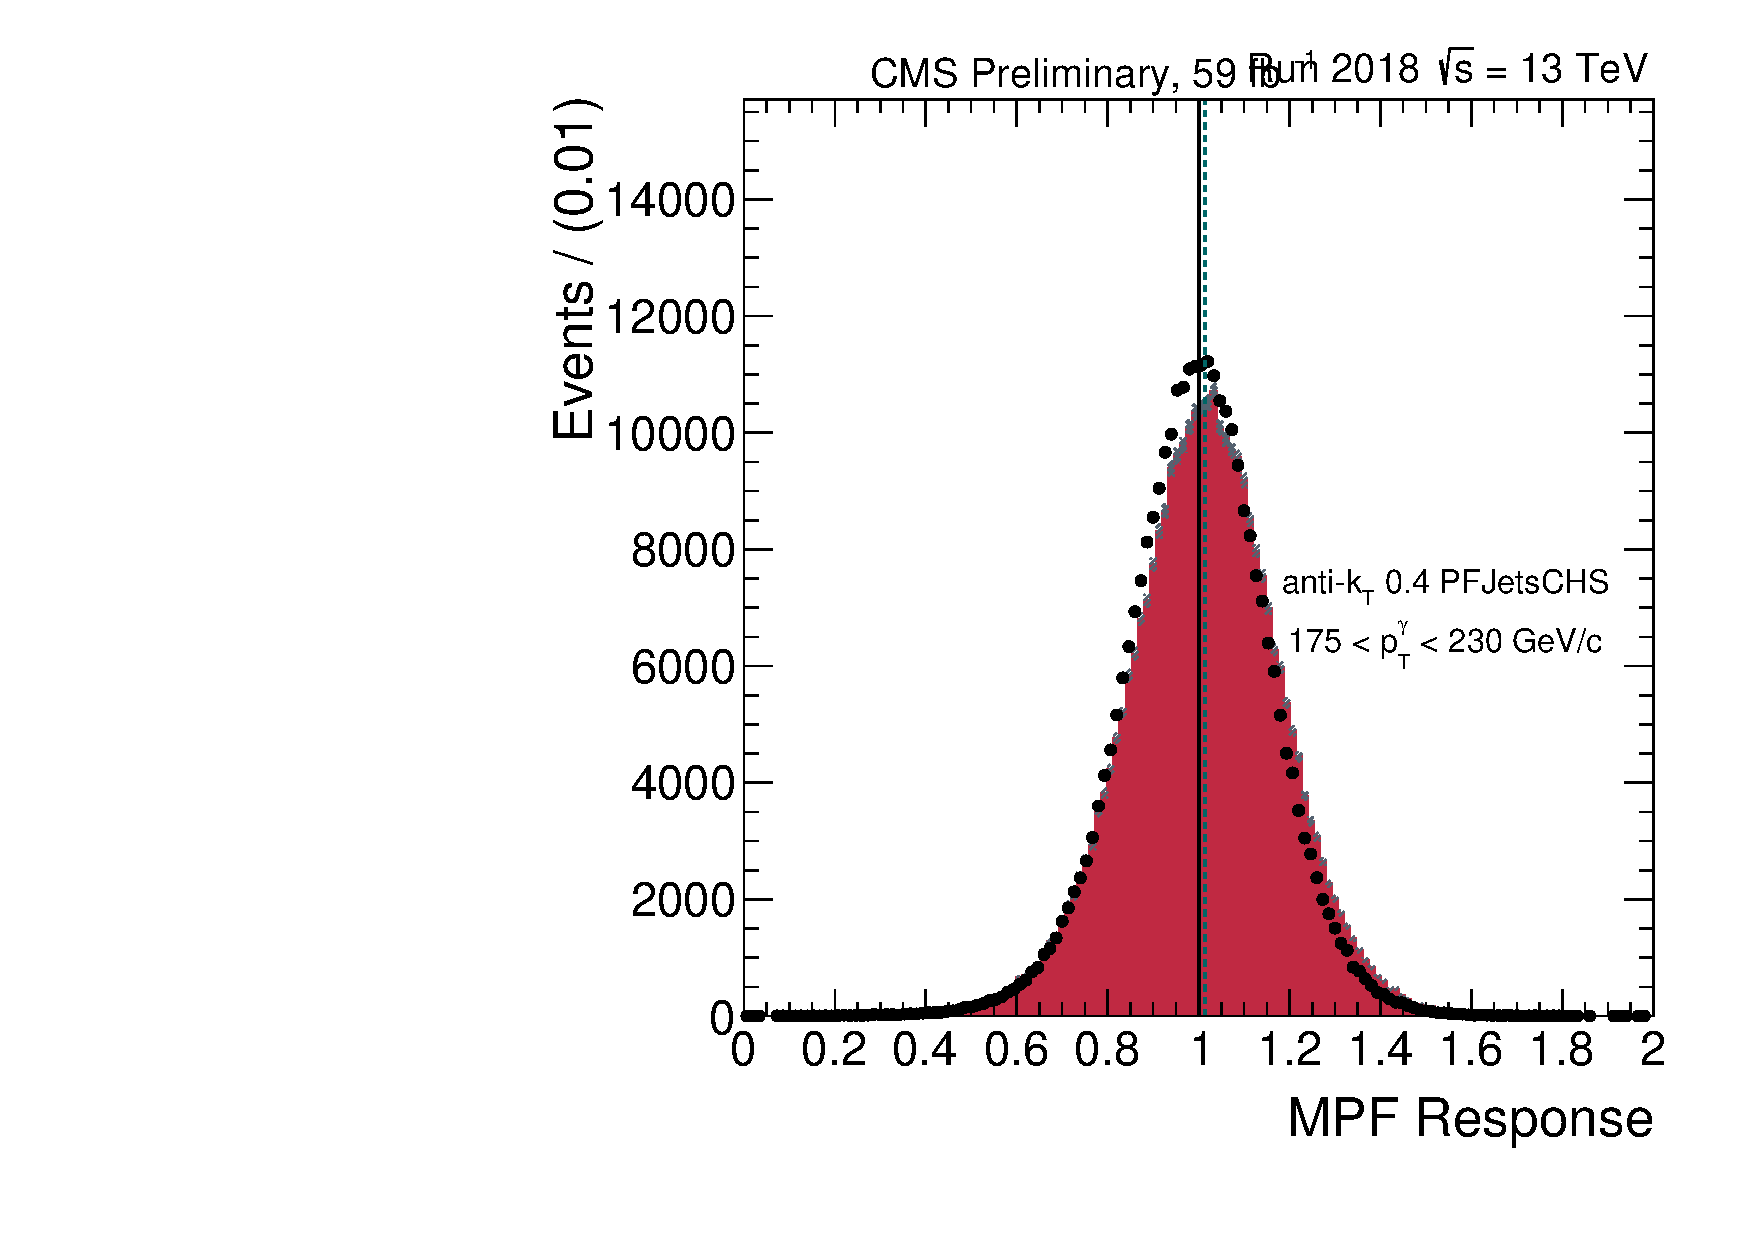
\includegraphics[width=.45\textwidth]{\PhDthesisdir/plots_and_images/my_plots/JERC/distributions/2018/with_header/resp_mpf_eta0013_ptPhot_175_230_L2L3Res.tex}}
\caption[Comparaison des réponses MPF avant et après correction résiduelle absolue en 2018.]{Comparaison des réponses MPF avant et après correction résiduelle absolue  pour $\pT^{\photon}\in[175, 230[$ \SI{}{\GeV} et $\abs{\eta}<\num{1.3}$ en 2018.}
\label{fig-distribs_Gjets_18_resp_mpf_L2L3Res_cross_check}
\end{figure}